% thesis?

\documentclass{report}
\usepackage{baththesis}

\usepackage{times, amsmath, amssymb, amsfonts, url, natbib, bm, rotating}
 
\usepackage{multirow}
\usepackage{graphicx}
\usepackage{rotating}
\usepackage{psfrag}

 
% Shortcuts
% Probability
\newcommand{\prob}[1]{\mathbb{P}\left[ #1 \right]}
% fprime
\newcommand{\fprime}{f^\prime(z)}
% phi inverse
\newcommand{\phiinv}{\phi^{-1}}
% use other phi
\renewcommand{\phi}{\varphi}
%transpose
\newcommand{\tr}[1]{#1^{\text{T}}}
% diagonal
\newcommand{\diag}{\text{diag}}
% call \times \cross
\newcommand{\cross}{\times}
% shortcut for ij^{th}
\newcommand{\ijth}{$ij^{\text{th}}$}


% references
% figure reference command
\newcommand{\fig}[1]{\emph{fig.} \ref{#1}}
% Figure reference command
\newcommand{\Fig}[1]{\emph{Fig.} \ref{#1}}
% table reference command
\newcommand{\tabref}[1]{table \ref{#1}}
% Table reference command
\newcommand{\Tabref}[1]{Table \ref{#1}}
% equation reference command
\newcommand{\eqn}[1]{(\ref{#1})}
% section references
\newcommand{\secref}[1]{section \ref{#1}}
\newcommand{\Secref}[1]{Section \ref{#1}}

% LaTeX laziness!
\newcommand{\bc}{\begin{center}}
\newcommand{\ec}{\end{center}}
\newcommand{\bn}{\begin{enumerate}}
\newcommand{\en}{\end{enumerate}}
\newcommand{\bi}{\begin{itemize}}
\newcommand{\ei}{\end{itemize}}
\newcommand{\be}{\begin{eqnarray}}
\newcommand{\ee}{\end{eqnarray}}
\newcommand{\bes}{\begin{eqnarray*}}
\newcommand{\ees}{\end{eqnarray*}}
\newcommand{\expect}[1]{\mathbb{E}\left[ #1 \right]}

% words
\newcommand{\sch}{Schwarz-Christoffel}
\newcommand{\tprs}{thin plate regression spline}

% whatever I call MDS+TP approach
\newcommand{\mdsap}{MDS+RS}

\title{Something something something statistical ecology(?)}
\author{David Lawrence Miller}
\degree{Doctor of Philosophy}
\department{Department of Mathematical Sciences}
\degreemonthyear{August 2011}

\norestrictions

\begin{document}

\maketitle
\begin{abstract} 
An abstract will go here.
\end{abstract}

%\newpage
%\begin{center}
%\vspace*{2in}
%\huge{AIEN API$\Sigma$TE$\Upsilon$EIN}
%\end{center} 

%\newpage
%\begin{center}
%\vspace*{2in}
%\huge{For $\mathcal{L}^*$.}
%\end{center} 

\tableofcontents

\listoffigures

\chapter{An Introduction}

Although this is called the intro, I've also but in bits that I want to put in that are general for more than one chapter. These are just bullet pointed \emph{aide memoirs} at the moment but will obviously be fleshed out in time.

\section{Statistical Ecology}

Some general remarks about stat ecol perhaps.

%\section{Themes}
%
%Some sort of general intro here.
%
%\bi
%	\item Morphing
%	\item Modifying penalties
%	\item Computational efficiency
%	\item Realistic physical models!!!!!!
%\ei


\section{Some notational conventions}


\section{Generalized Additive Models}

General GAM setup. The is will mostly be taken from \cite{simonbook}, \cite{rwc} and \cite{marraradice2010}.

\bi
\item Splines
\item objective function
\label{GAMobjfcn}
\item penalties
\label{GAMpenalties}
\item bases - TPRS (and maybe P-splines?)
\label{GAMtprspenalty}
\item fitting - GCV REML etc
% see p. 122 RWC here GCV vs REML -> same MSE but different tradeoffs in Var and Bias
\item other stuff - MSE, EDF etc
\item \texttt{mgcv}
%	\bi
%	\item MSE
%	Mean squared error is... (look at HTF)
%	
%	\begin{equation}
%\text{MSE}(\hat{f}) = \frac{1}{P} \sum_{j=1}^P (\hat{f}(x_j) - z_j)^2,
%\end{equation}
%the mean difference between the model ($\hat{f}$) evaluated at the prediction points ($\{x_j : j=1 \dots P\}$) and the true value of the function ($\{z_j : j=1 \dots P\}$.) This gives the MSE per model, since here many realisations are run, the mean of these over all simulations is taken and the standard error is calculated.
%	\item EDF
%	
%The estimated degrees of freedom gives an measure of the complexity of the model that was fit to the data. The higher the EDF, the more basis functions were used and  the more complex the model.  Since the models used here are penalised, it is the penalty term that controls the overall ``wigglyness'' of the spline and hence the EDF. Although the basis dimension is set in the model, this is just an upper bound, the smoothing penalty suppresses parts of the model. Therefore basis dimension is not a major concern provided that it is not set too low (\cite{simonbook}, p. 161.) 
%
%	\ei
\ei

\section{Finite area smoothing}

\subsection{Overview of finite area smoothing}

Splines are a popular way of performing spatial smoothing in two dimensions. In this context, they are often used to fit smooth functions over a geographical region. A typical application of this is in ecological modelling; a response (be it simply the presence of individuals in a population or concentration of a chemical) is modelled as a function of its spatial coordinates. The estimated function can then be used to perform inference on the population, whether that be an abundance estimate, density map or a more sophisticated inferential goal. Finite area smoothing simply specifies that the domain over which this smoothing takes place is bounded.

When the geographical region has a \emph{complex boundary}, features from one part of the domain can unduly influence other parts. Considering the boundary as a polygon, a complex boundary is a non-convex polygon, in particular when the non-convexity is relatively extreme. Often this consists of having some peninsula-like feature(s) in the domain with notably different observation values on either side of the feature. Given that there is some scientific motivation as to why those parts of the domain should not affect each other, features such as peninsulae give rise to a phenomenon known as \emph{leakage}.

Leakage occurs when a smoother inappropriately links two pats of a domain (\cite{soap}). The phenomenon is problematic since it causes the fitted surface to be mis-estimated; this can then lead to incorrect inference (eg. biased abundance estimates), which is clearly not desirable. Leakage can be seen in \fig{leakage} where the high values in the upper half of the domain leak across the gap to the lower values below and vice versa.

% leakage example 
\begin{figure}
\centering
% trim order l b r t
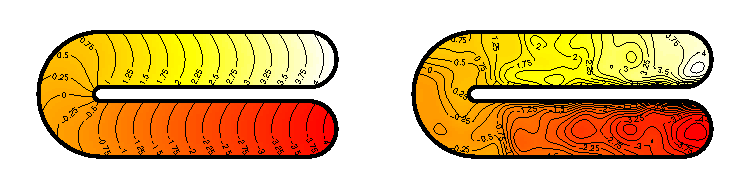
\includegraphics{intro/figs/ramsay-leak.pdf}\\
\caption{An example of leakage. A thin plate regression spline was fit to data sampled from the function on the left, here the model smooths across the gap in the middle of the domain (right.)}
\label{leakage}
\end{figure}

The problem of leakage arises because of the way in which the smoother defines how near objects are to one another. Most smoothing techniques use the Euclidean metric to measure the distance between data. Clearly though, this approach is a flawed: biological populations do not conform to Euclidean geometry in their movement patterns and hence their observed positions will reflect this. Just as whales no not uniformly distribute themselves across sea and glacier, fish do not lay their eggs on land. Natural and man-made barriers carve up the landscape (and seascape), partitioning biological populations; our models should take this into account.

The distribution of the population may be smooth, just not necessarily over $\mathbb{R}^2$ (\cite{wangranalli}). Instead the structure of the domain that is under investigation must be modelled (implicitly or explicitly) for the correct inference to be drawn.

\subsection{Ramsay's horseshoe function as a benchmark for finite area smoothing}

\label{ramsayfunc}

\cite{ramsay} proposes a function which can be used to benchmark new approaches to 2-dimensional smoothing. The function takes the form of a horseshoe shape which is flat across the domain has a gradient along the domain's major axis. This can be seen in \fig{orig-fs}. \cite{soap} modifies the test function by adding curvature across the minor axis of the shape. This was added in order to avoid the horseshoe function lying in the nullspace of their model's penalty, making the problem trivial. It is the second shape that will be used for simulations here and shall be referred to as the \emph{Ramsay horseshoe} throughout; it is shown in \fig{leakage}.

% original horseshoe from Ramsay's paper
\begin{figure}
\centering
% trim order l b r t
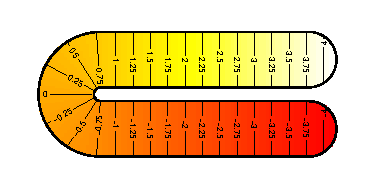
\includegraphics{intro/figs/orig-fs.pdf}\\
\caption{The horseshoe function as it appeared in \cite{ramsay}.}
\label{orig-fs}
\end{figure}

The test function highlights leakage well. As mentioned above, when the smoothing problem is specified in Euclidean distance, the model takes the distance between the points in the two arms of the horseshoe as the distance over the gap in-between them, rather than the distance along the major axis of the shape. This causes the high function values from one side to contaminate the other side (and the low to contaminate the high.) It is easy to see that this causes the smooth to be an inappropriate model.
		
\subsection{Previous approaches to leakage}

The cause of leakage can be characterised in two ways: either the smooth does not respect the boundary of the domain, or the smooth does not take into account the geometry of the domain (in particular with regard to the distance between points within the domain). Previous work in this area has been to combat leakage along these two lines. Work of \cite{ramsay} and \cite{soap} both use a partial differential equation (PDE) boundary condition approach to try to prevent leakage, where as \cite{wangranalli} and \cite{eilerstalk}  attempt to approximate the intrinsic structure of the domain while not treating the boundary as something special in the basis setup. These four main works may be summarised as follows:

\begin{enumerate}
\item \cite{ramsay} proposes finite element $L$-splines (FELSPLINEs). The $L$-spline replaces the usual penalty term (see \secref{GAMpenalties}) with:
\be
\int_\Omega (L_p f)^2 \text{d}\Omega,
\ee
where $\Omega$ is the domain in question and $L_p$ is a roughness operator defined as:
\be
L_p=\Delta^p+c_{p-1}\Delta^{p-1}+\dots+c_1\Delta+c_0I.
\ee
Here $I$ is the identity operator, the $\{c_0,\dots, c_p\}$ are constants and the $\Delta$ is the Laplacian ($\Delta f = f_{xx}+f_{yy}$ in the usual notation). Although any differential operator could, in principle, be used for $L_p$, the Laplacian gives rise to a set of polynomials which are rotation and translation invariant which is clearly sensible given the objective function solution should not depend on the coordinate system used.

In order to find the minimiser of the objective function, Ramsay takes a finite element approach. First he triangulates the domain, then he constructs a set of bivariate quadratic polynomial basis functions over each triangle, specifying that there be continuity over the edges of the triangles. By taking the FELSPLINE objective function and transforming it into a variational form (in the same way as a PDE is), the approximation to the minimiser of the objective function is found. 

Since the triangulation and hence the penalty of the FELSPLINE is only calculated over the domain, and the continuity is specified over neighbouring cells, the method prevents leakage. However, although FELSPLINE does not exhibit leakage on the original horseshoe (as in \fig{orig-fs}), in practice the model makes unrealistic physical assumptions. The boundary conditions of FELSPLINE specify that the gradient is zero, along normals to the boundary. This is not always physically realistic. \cite{soap} show that by using a different response function for the horseshoe shape, the FELSPLINE performance begins to falter.

FELSPLINE does not offer a realistic physical model and is therefore not a viable solution to the finite area smoothing problem in general.

\item \cite{wangranalli} adopt a ``within-area distance'' formulation for thin plate splines. They take the geodesic distance between two points, that being the shortest path within the domain. This gives a definition of how near objects are in the domain. 

Wang and Ranalli first create a weighted, undirected graph ($G$, say) with a data point at each vertex and the distance between each pair of vertices as the weights on the edges. They then take the restricted graph of $G$, $G_k$, in which each vertex is only connected to its $k$ nearest neighbours. With this new, restricted graph the geodesic distances between each pair of vertices can be calculated using Floyd's algorithm (\cite{Floyd}).

As the authors point out, the quality of the approximation is dependent on the size of the data set and its density. At low densities the estimated geodesic distance will tend towards the Euclidean, at high densities the approximation tends, asymptotically toward the true geodesic distance (\cite{bernstein}). Even if  dense enough data were available, the method will be rather slow since Floyd's algorithm is cubic in the number of vertices (the size of the data set). Finally, although the $k$-nearest neighbours algorithm used is not specified in the paper, in general such procedures are computationally expensive, adding another source of impedance to the technique.

Taking these points into account, Wang and Ranalli's approach appears cumbersome, slow and dependent on dense data.

\item The soap film smoother (\cite{soap}) uses a rather simple physical model to prevent leakage from occurring. First, consider the domain boundary to be made of wire, then dip this wire into a bucket of soapy water, you will then have (provided it doesn't pop(!)) a soap film in the same of your boundary. Now consider the wire to lie in the $x-y$ plane and the height of the soap film at a given point to be the functional value of the model. This film is then distorted smoothly by moving it toward the data, while minimising the surface tension in the film. The domain ($\Omega$) is bounded by some polygon with boundary conditions that are either known or estimated by a cyclic spline.

Mathematically, the soap film smoother is constructed by first specifying a set of functions $\rho_k(x,y)$, which are each solutions to the Laplace equation in two dimensions:
\be
\frac{\partial^2\rho}{\partial x^2} + \frac{\partial^2\rho}{\partial y^2} = 0
\ee
except at one of the knots ($x^*_k,y^*_k$). Then, solving Poisson's equation in 2-dimensions:
\be
\frac{\partial^2 g_k}{\partial x^2} + \frac{\partial^2 g_k}{\partial y^2} = \rho
\label{soap-poisson}
\ee
with $\rho=\rho_k(x,y)$, where $k$ indexes the knots and the boundary condition $\rho=0$. The set of basis functions for the soap film smoother, $g_k(x,y)$ is found, along with $a(x,y)$ (the solutions to \eqn{soap-poisson} when $\rho=0$, subject to the boundary condition). These bases are then summed to form:
\be
f(x,y)=a(x,y)+\sum_{k=1}^n \gamma_k g_k(x,y),
\ee
the soap film smoother, where the $\gamma_k$ are parameters to be estimated. The (isotropic) penalty term (\secref{GAMpenalties}) is:
\be
\int_\Omega \Big(\frac{\partial^2 f}{\partial x^2}+\frac{\partial^2 f}{\partial y^2} \Big)^2\text{d}x\text{d}y,
\ee
Differing from the standard \tprs penalty since: (\emph{i}) the integration occurs only over $\Omega$, (\emph{ii}) there is no mixed derivative term, and (\emph{iii}) the whole integrand is squared rather than each term individually. This allows the $x$ and $y$ term's derivatives to be traded off against each other so the nullspace of the penalty is infinite dimensional. This allows those functions in the nullspace to be sufficiently wiggly to meet any boundary conditions.

The solution of the PDEs above, yielding the basis and penalty, is the most computationally expensive part of the procedure. Knots to use for $x_k^*$ and $y_k^*$ must be specified, usually using a grid. Numerical problems occur when knots are placed in boundary cells in the PDE solution grid.

Although mathematically elegant, the soap film smoother is a rather complex model. It also treats the boundary differently from the interior and uses a cyclic spline in order to approximate the boundary values. This treatment of the boundary seems rather unnatural and it may not always be physically realistic to consider the boundary in such a way.

\item An alternative approach to treating the boundary as something special is to transform the space in which the points lie to instead lie in a different domain which is more suitable for smoothing. For example, with Ramsay's horseshoe, it seems intuitive to simply bend the horseshoe into a long strip and then smooth on that domain.

Indeed, \cite{eilerstalk} proposed using the \sch transform for this very purpose (I, independently, came to the idea in 2008 via BBC Radio 4.) Using the \sch transform for smoothing will be elaborated on in chapter \ref{chap-sc}, so only a brief summary is given here.

The basic idea is to find a function, $\phi$ say, that takes points in the domain the data lie in ($W$) and maps them to a domain ($W^*$) in which the boundary is less complex ($\phi : W \mapsto W^*$, mathematically).

Creating some kind of mapping between the space in which the data lies and the space in which conventional smoothers perform well is convenient. Not having to setup a new basis structure and relying on long tested methodology is clearly appealing. This approach also benefits from not treating the boundary as a special in the basis setup.
\end{enumerate}

Chapters \ref{chap-sc} and \ref{chap-mds} expand on the ideas in the last method; of using a transformation of space and conventional smoothers to solve the problem of leakage in finite area smoothing.

\section{Distance sampling}

This will be a very brief introduction to distance sampling methods, in the style of the encyclopaedia of environmetrics article.


\chapter{The \sch\ transform as a method for finite area smoothing}
% "failure is always an option" - Adam Savage

% schwartz-christoffel stuff

\label{chap-sc}

\section{Introduction}

This chapter investigates the efficacy of using a conformal mapping to transform the domain in which we wish to perform smoothing. The mapping takes points in the domain of the data ($W$) to a domain on which it is easier to smooth ($W^*$). In particular the utility of the \sch transform is examined (elaborating on \cite{eilerstalk}).

Given some region that it is difficult to smooth over, one approach is to transform the domain in which the problem resides. So, for example, one could transform a region into a rectangle, circle or other familiar shape to avoid the problems such as leakage. In this spirit, we wish to find some mapping such as $\phi$ in \fig{simpledia}.

This kind of approach is appealing since it allows the use of existing techniques in the transformed domain (\emph{ie.} not having to resort to model and basis reformulation). It also feels more natural to treat the domain as if it were made of silly putty and simply squash the region into the shape required to perform analysis.

% Simple diagram showing the mapping
\begin{figure} [htbp]
\centering
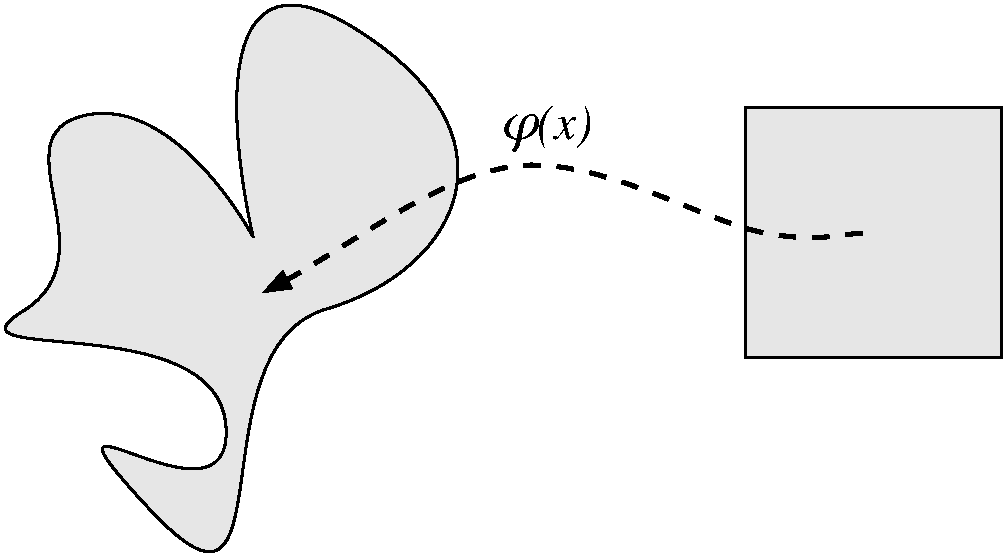
\includegraphics[scale=0.3]{sc/figs/simpledia.pdf}
\caption{An example of a transformation; the function $\phi$ takes the points in the rectangle and maps them to the region on the left.}
\label{simpledia}
\end{figure}

The \sch mapping offers such a transformation; it takes some arbitrary polygon and maps it to some specified shape. The most common domains to transform to are: (i) the upper half-plane ($H^+$), (ii) a rectangle and (iii) the unit disk. This is achieved in the $H^+$ case by taking the vertices of the polygon and mapping them to points on the real line (see \fig{reallinedia}). This can be thought of as ``unwrapping'' the polygon onto the real line. For the unit disk case, points on the circle bounding the unit disk map to vertices on the polygon (see \fig{unitdiskdia}). One can think of this as adding control points to the unit circle and then altering the angles. The rectangular case is somewhat similar to the unit disk in that extra points are added to the boundary and the angles of these points tightened until the shape is identical to the polygon. Obviously, those points lying inside the polygon are also moved around due to the mapping, creating a new (non-uniform) distribution of space.

% Diagram showing upper half plane to polygon
\begin{figure} [tbp]
\centering
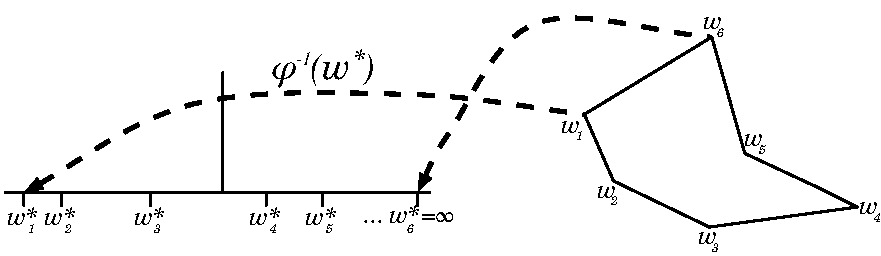
\includegraphics[scale=0.6]{sc/figs/reallinedia.pdf}
\caption{A mapping of the upper half-plane to the polygon. The vertices ($w_k$) are the result of applying $\phi$ to the points on the real line ($w^*_k$). The boundary of the polygon is mapped to the real line. Note that the final vertex, $w^*_6$ is mapped to the point $\infty$ on the real line.}
\label{reallinedia}
\end{figure}

% Diagram showing unit disk to polygon
\begin{figure} [tbp]
\centering
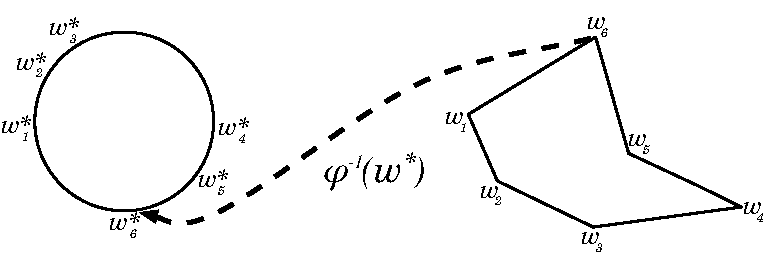
\includegraphics[scale=0.6]{sc/figs/unitdiskdia.pdf}
\caption{A mapping of the upper half-plane to the polygon. The vertices ($w_k$) are the result of applying $\phi$ to the points on the real line ($w^*_k$). The boundary of the polygon is mapped to the boundary of the unit disk.}
\label{unitdiskdia}
\end{figure}

The goal is to transform the domain with the complex boundary, then smooth in the transformed domain. The procedure we wish to perform is as follows:

\begin{enumerate}
\item Determine the domain over which we would like to smooth, $W$. This could be the region or a bounding box around it.

\item Compute the \sch transform of $W$ to get $W^*$. Obtaining the function, $\phi$.

\item Map the co-ordinates of the datapoints in $W$ to $W^*$.

\item Smooth the data in $W^*$.

\item Perform any further inference (in $W$ or $W^*$, since there is a 1-1 mapping between them).
\end{enumerate}

The second section of this chapter explains the technical details of the mapping. The third section gives results of some simulations and the final section summarises the results and draws conclusions from them.

\section{Technical details}

This section gives some of the mathematical and computational details required to calculate the \sch mapping. The primary reference is the extremely thorough work of \cite{driscoll}, which covers almost all aspects of the \sch transform.

\subsection{Nomenclature}

The polygon is first defined formally along with its associated quantities, as they will be referred to throughout the rest of the chapter.

A polygon, $\Gamma$, is a collection of vertices $w_1, w_2,\dots,w_n$ and interior angles $\alpha_1\pi, \alpha_2\pi, \dots, \alpha_n\pi$. For convenience we define $w_{n+1} = w_1$ and $w_0=w_n$. Numbering of vertices is anti-clockwise. The angles are such that $\alpha_k \in (0,2]$ and we require:
\begin{equation}
\sum_{k=1}^n (1-\alpha_k) = 2.
\end{equation}
The external angle, $\theta_k\pi$, as given by $(1-\alpha_k)\pi$ (see \fig{anglediagram}).

% Diagram showing the exterior/interior angle relationship.
\begin{figure} [bp]
\centering
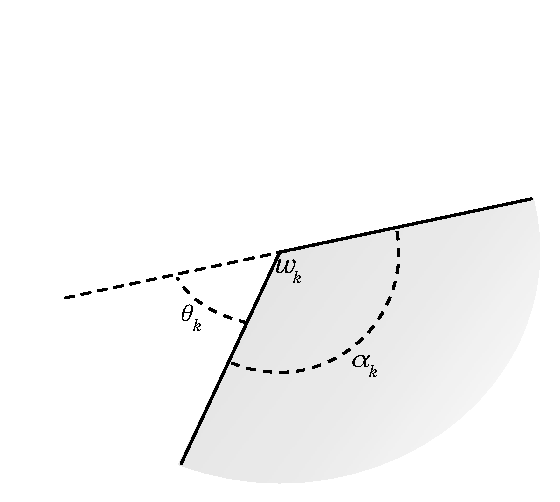
\includegraphics[scale=0.6]{sc/figs/anglediagram.pdf}
\caption{The external angle $\theta_k$ is associated with the vertex $w_k$. The internal angle is given by $\alpha_k$. Shading indicates the inside of the polygon.}
\label{anglediagram}
\end{figure}

The boundary of the polygon is denoted by $\Gamma$. We refer to two domains: $W$ and $W^*$, denoting the original domain (inside $\Gamma$) and the transformed domain (of the plane, unit disk or rectangle) respectively. 

Vertices on the polygon are denoted as $w_k$ and those on the transformed boundary are denoted as $w^*_k$ (the \emph{prevertices}). In general a point in the polygon's original domain is denoted as $w$ and in the transformed domain as $w^*$.

We use the function $\phi$ to map from the transformed domain to the polygon (\emph{ie.} $\phi:W^* \mapsto W$). The inverse mapping function, $\phi^{-1}$, is used to go from the polygon to one of: the unit disk, rectangle or half-plane ($\phi:W \mapsto W^*$).  See \fig{mappingdia}.

% Mapping diagram from my whiteboard
\begin{figure} [tbp]
\centering
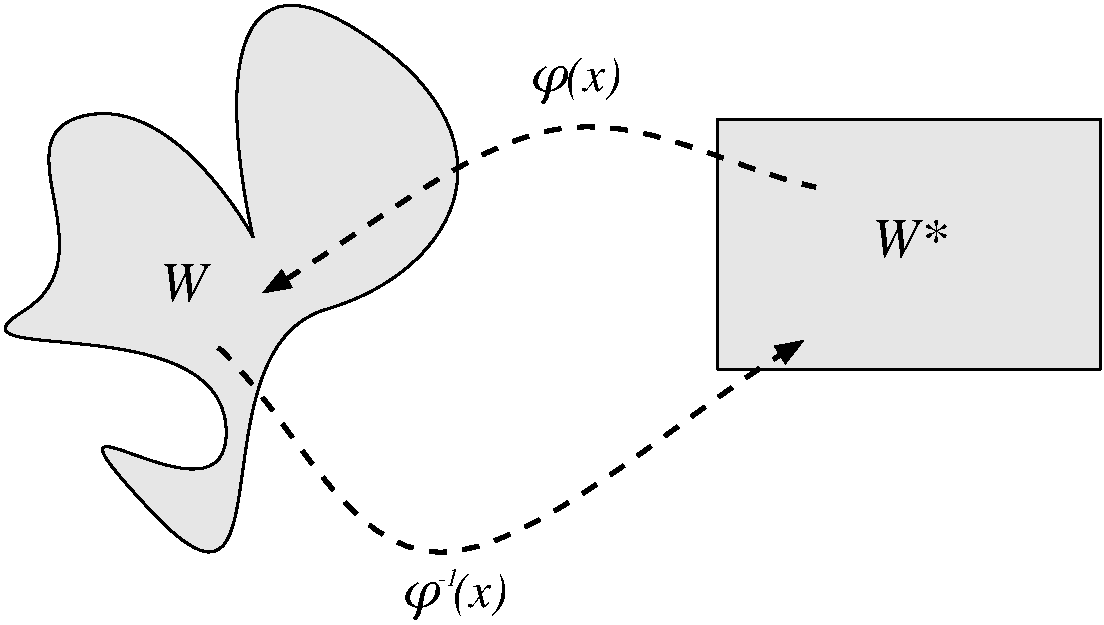
\includegraphics[scale=0.5]{sc/figs/mappingdia.pdf}
\caption{Diagram showing the forwards and backwards mappings with their relations to the mapped and unmapped spaces in the rectangular case.}
\label{mappingdia}
\end{figure}

\subsection{\sch Mapping}
\label{schparprob}
We now look at the mathematical formulation for the upper half-plane, unit disk and rectangle. There are many mappings that can be performed however those detailed here are either canonical (in the case of the half-plane) or considered to be useful in a smoothing context (the other two).

For the purposes of smoothing we are interested in the function $\phi^{-1}$ (\emph{ie.} the function that goes from our domain to the transformed one). We must first calculate $\phi$ before we may calculate its inverse. In the literature $\phi$ is referred to as the \emph{forwards map} and $\phi^{-1}$ as the \emph{backwards map}.

The forwards map, $\phi$, is determined up to translation, scaling, and rotation by the prevertices (see below). So, our task is to efficiently find the prevertices and hence find the mapping $\phi$. The task of obtaining the prevertices is known as the \emph{\sch parameter problem}.

\subsubsection{The upper half-plane}
\label{sc-parprob}

When mapping $\Gamma$ to $H^+$ we set $\phi(\infty) = w_n$ without any loss of generality. \cite{driscoll}, p. 10 then gives the following formula formula:
\begin{equation}
\phi(w^*) = A + C \int^{w^*}_{w^*_0} \prod_{k=1}^{n-1} (\zeta-w^*_k)^{\alpha_k-1} d\zeta.
\end{equation}
Here $A$ and $C$ are complex constants determined once the $w^*_k$ have been calculated. These control the scaling, translation, and rotation of the transform.

Although setting $\phi(\infty) = w_n$ does not make any difference in a mathematical sense, it does mean that the density of the points mapped into $H^+$ is rather odd. Given two adjacent points near $w_n$, their spacing on the upper half-plane is huge in comparison to two adjacent points near the other vertices. For this reason the $H^+$ mapping is not pursued further here.

\subsubsection{Unit disk}

The formula for the unit disk looks very similar to that for $H^+$ but the product now runs over all prevertices. The integrand is simply a constant multiple of the $H^+$ case. This is merely to avoid problems in the calculation of the branch cuts (\cite{driscoll}, p. 12).
\begin{equation}
\label{unitscmap}
\phi(w^*) = A + C \int^{w^*}_{w^*_0} \prod_{k=1}^{n} (1 - \frac{\zeta}{w^*_k})^{\alpha_k-1} d\zeta.
\end{equation}
As above, $A$ and $C$ are complex constants responsible for scaling, translation, and rotation.

\subsubsection{Rectangle}
For the rectangle case we must specify four vertices of $\Gamma$ that map to the four corners of the rectangle. This uniquely specifies the aspect ratio of the rectangle (\cite{driscoll}, p. 48).

The rectangle mapping is slightly different in its calculation to the two above mappings. We first map $\Gamma$ to the upper half-plane as detailed above. From there we can use the Jacobi elliptic function (\cite{handbuch} p. 701):
\be
F(\gamma,k)=\int_0^\gamma \frac{dt}{\sqrt{1-k^2\sin^2t}}
\ee
to map a rectangle to the upper half-plane. The computation of this map is expensive due to the evaluation of the elliptic function (\cite{driscoll}, \emph{p. 49}) so a shortcut is used by mapping to the strip. We do not go into further about detail here (as the computational intricacies are covered in \cite{howell90}).

\subsection{Computation of the \sch mapping}

To compute the map, we need to find the prevertices, $w^*_k$; since the complex constants just control scaling, translation, and rotation, we can compute them after computing the $w^*_k$. We achieve this iteratively by approximating the $w^*_k$ then mapping those points back to the polygon to give an estimate to $\Gamma$, $\Gamma^\prime$. 

To measure the quality of approximation of $\Gamma^\prime$ to $\Gamma$ we use the following set of equations:
\begin{equation}
\label{optimizeme}
\frac{\vert \phiinv(w_{k+1}) -  \phiinv(w_k) \vert}{\vert \phiinv(w_2)-\phiinv(w_1)\vert} - \frac{\vert w^*_{k+1} - w^*_k\vert}{\vert w^*_2 - w^*_1\vert} = 0, \qquad \text{for } k=3,\dots,n-1.
\end{equation}
Here $\vert \phiinv(w_{k+1}) -  \phiinv(w_k) \vert$ is the distance between the $k^{\text{th}}$ and $(k+1)^{\text{th}}$ vertex.  We find this by integrating along the line between the points within $W$.

Intuitively, we are comparing the side lengths of the polygon in order to evaluate approximation of $\Gamma$ in each iteration (\cite{snider}, A-3). Both of these measures are scaled by the distance between the first two vertices (in their respective domains).

Note that \eqn{optimizeme} does not include the vertex $w_n$. By theorem 3.1 of \cite{driscoll}, p. 24) a polygon is precisely defined by its angles and its vertices not including $w_n$ (since if we know the direction of the edges leaving $w_1$ and $w_{n-1}$, we may find the point where they meet). It is for this reason, in the upper half-plane case, that we can map $w_n$ to $\infty$ without loss of generality.

Also note that \eqn{optimizeme} does not include $w_1$ or $w_2$ in the numerator on the right hand side. This is due to all vertices (and hence $w_1$ and $w_2$) being rescaled, rotated, and translated by the complex constants, $A$ and $C$, in the \sch formula.

In practice we fix $w^*_n=1$, $w^*_{n-1}=-i$ and $w^*_{n-2}=-1$ in the unit disk case (\cite{driscoll}, p. 24). For the rectangle case we need to specify which vertices of $\Gamma$ will map to which vertices of the rectangle.

The scaling factor, $C$, (from \eqn{unitscmap}) may be calculated using:
\begin{equation}
C=\frac{\vert \phiinv(w_2)-\phiinv(w_1)\vert}{\vert w_2 - w_1\vert}.
\end{equation}
Otherwise, we can assume that up to scaling and rotation that $w_1$ and $w_2$ are correct. In which case we know that $\Gamma$ and $\Gamma^\prime$ are similar (in the geometric sense). 

$A$ is the image of the base point of the integration and is usually written as $w_0$. For computational reasons this is usually the prevertex nearest to the point $w^*$ that we wish to map in \eqn{unitscmap}  (\cite{driscoll}, \emph{p. 27}).


\subsubsection{Sketch of an algorithm to calculate the \sch mapping}
\label{algorithmsketch}
\begin{enumerate}
\item Accept inputs:
   \begin{enumerate} 
      \item $w_1,\dots,w_n$ (the vertices),
      \item $n$ (the number of vertices),
      \item $\alpha_1,\dots,\alpha_n$ (the internal angles at each vertex).
   \end{enumerate}
\item Define the objective function, $F$, as:
 \begin{equation*}
F=\frac{\vert \phiinv(w_{k+1}) -  \phiinv(w_k) \vert}{\vert \phiinv(w_2)-\phiinv(w_1)\vert} - \frac{\vert w^*_{k+1} - w^*_k\vert}{\vert w^*_2 - w^*_1\vert}, \qquad \text{for } k=3,\dots,n-1,
 \end{equation*}
\item Use steepest descent and then Newton's method to until $\vert F\vert < \epsilon \quad \forall k$. \item Calculate $C$ and $A$ as detailed above.
\item Return values for $w^*_1,\dots,w^*_n$, $C$ and $A$.
\end{enumerate}

Starting values for the algorithm are evenly spaced vertices around the edge of the disk/rectangle or, in the case of the plane, along the real line. Not including those vertices specified as being fixed, above.

\subsection{Getting between $W$ and $W^*$}

\subsubsection{Forwards map}

Calculating the forwards map is simply a case of evaluating $\phi$ at the necessary points. If we wish to find the point on polygon ($w$), given some known point on the disk ($w^*$), we compute:
\begin{equation}
\label{forwardsmap}
w=\phi(w^*) = w_0 + C \int_{w^*_0}^{w^*} \prod_{k=1}^{n} (1 - \frac{\zeta}{w^*_k})^{-\theta_k} d\zeta,
\end{equation}
where $w^*_0$ is any point in the closed disk such that $w_0 = \phi(w^*_0)$ is known and non-infinite. We may choose any point since the integrand is analytic throughout the mapping and hence the integral is path-independent (\cite{driscoll} \emph{p. 27}). A common choice for $w_0$ is the centre of the polygon.

Equivalent expressions exist for the rectangle and upper half-plane cases (see \cite{driscoll} p. 49 and p. 10, respectively).

\subsubsection{Backwards map}

To calculate the backwards mapping, there are two possible approaches: (i) using Newton's method to solve the equation $\phi(w^*)-w=0$ and (ii) solving the initial value problem (IVP):
\begin{equation}
\label{scivp}
\frac{dw^*}{dw}=\frac{1}{\phi^{-1}(w^*)} \quad \text{and} \quad \phiinv(w_0)=w^*_0.
\end{equation}
In fact a combination of these methods are used. Solving \eqn{scivp} approximately gives the starting values for the Newton iterations which are significantly faster (since $\phi^{-1}$ is cheaper than $\phi$ to compute) (\cite{driscoll} p. 29).

The only problem with this is that the path from $w_0$ to the point to map, $w$, must lie entirely inside the polygon. Whether this is true is not known, since after the mapping has been computed, the only known points are the vertices (at which the IVP is singular). So, to combat this, all points on the path are checked sequentially. This computation, although inelegant, is fast compared to the IVP/Newton iterations.

An example of using the backwards map to find the transformed co-ordinates from a square to the unit disk is given in \fig{squaredomain}. An irregular nonagon is given in \fig{irregdomain}.


% Square domain mapping diagram
\begin{figure} [bp]
\centering
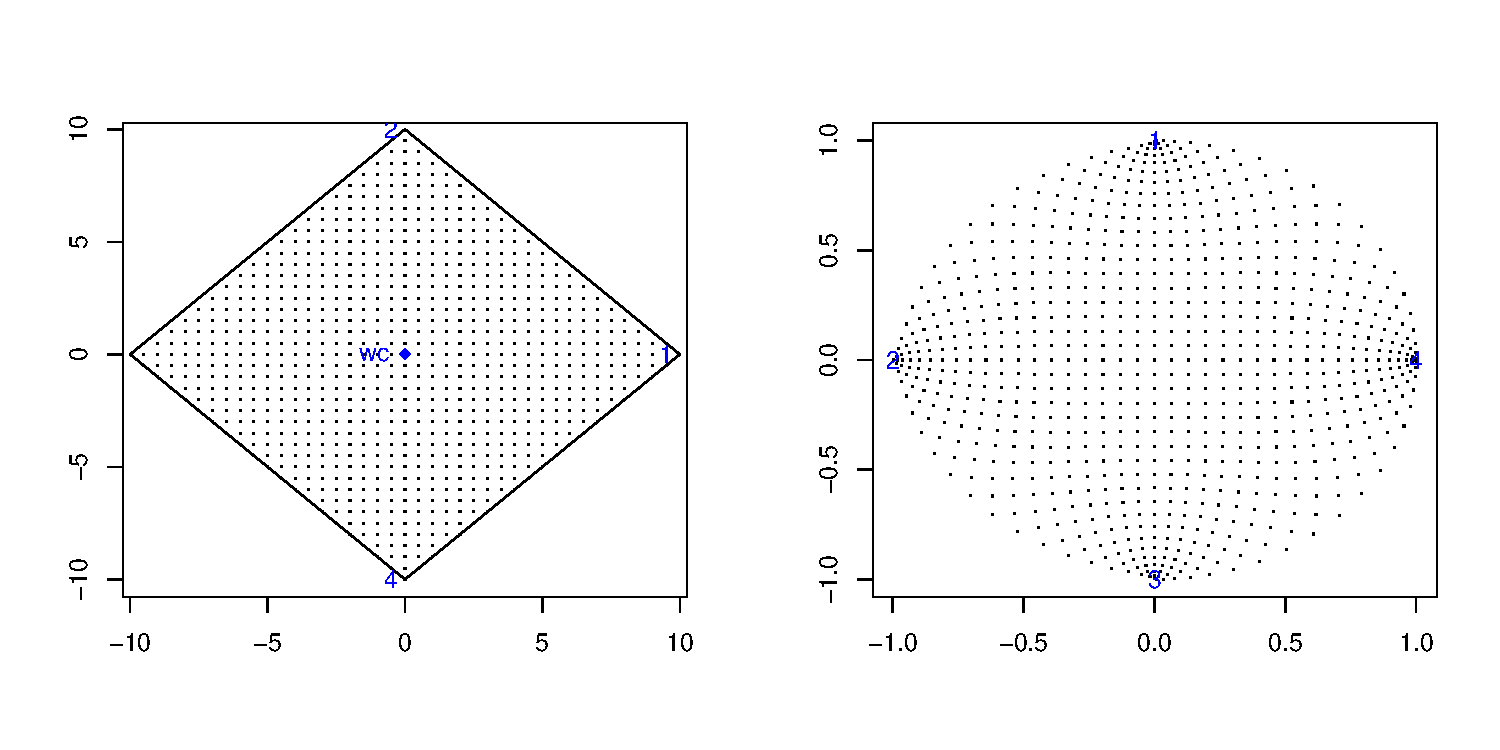
\includegraphics[scale=0.5]{sc/figs/squaredomain.pdf}
\caption{A regular grid of points over the square region (left). The right panel shows the mapping of these points under the \sch transformation to the unit disk.}
\label{squaredomain}
\end{figure}

% Irregular mapping diagram
\begin{figure} [tbp]
\centering
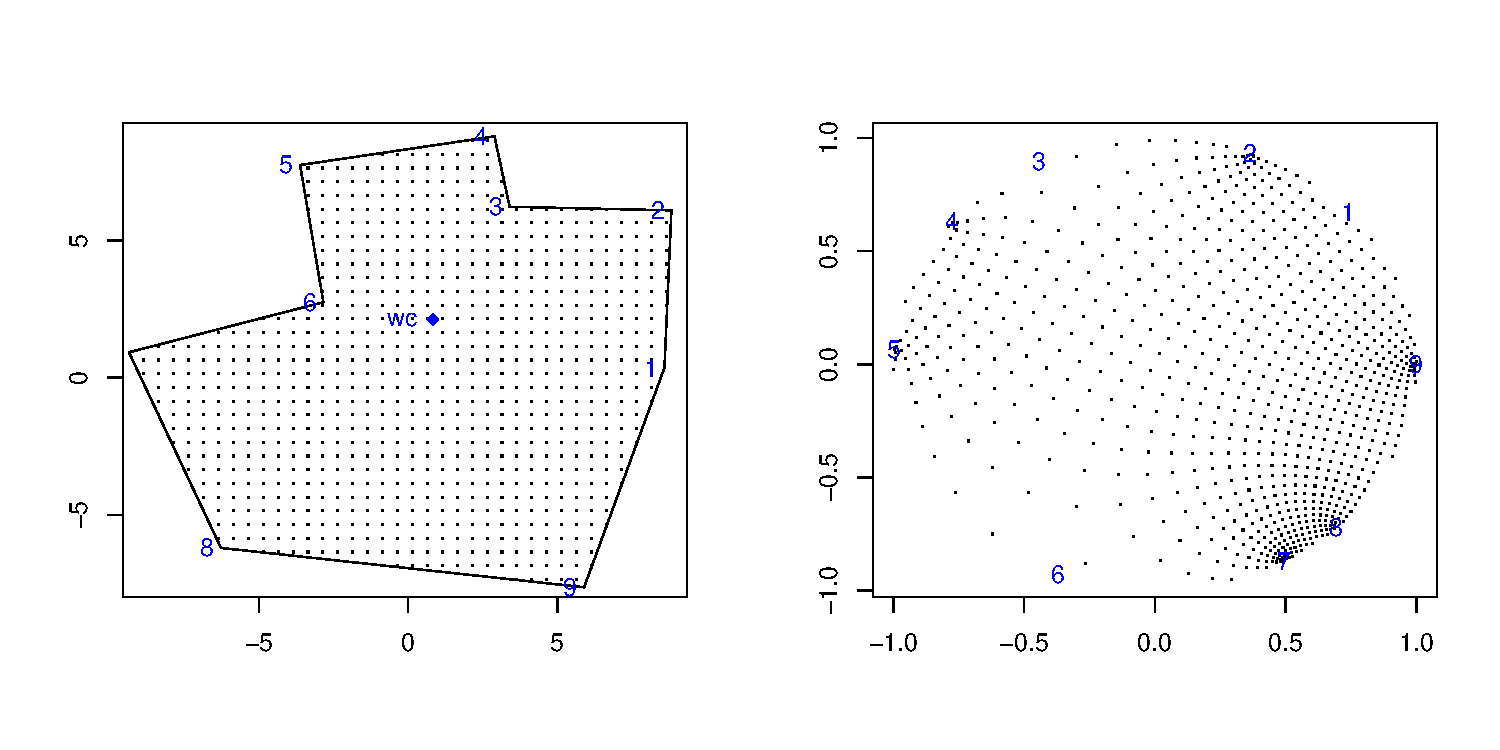
\includegraphics[scale=0.5]{sc/figs/irregulardomain.pdf}
\caption{A regular grid of points over region bound by a irregular nonagon (left). The right panel shows the mapping of these points under the \sch tranformation to the unit disk.}
\label{irregdomain}
\end{figure}

\subsection{Crowding}

\subsubsection{The crowding problem}
When the polygon is elongated or has many vertices, the mapped vertices may be positioned too closely in the transformed domain. This effect is referred to as \emph{crowding} and can be observed in \fig{crowdeddisk}. In elongated regions prevertices can be located exponentially close such that they are indistinguishable in finite precision arithmetic (\cite{howell90}).

% Crowded mapping diagram
\begin{figure} [tbp]
\centering
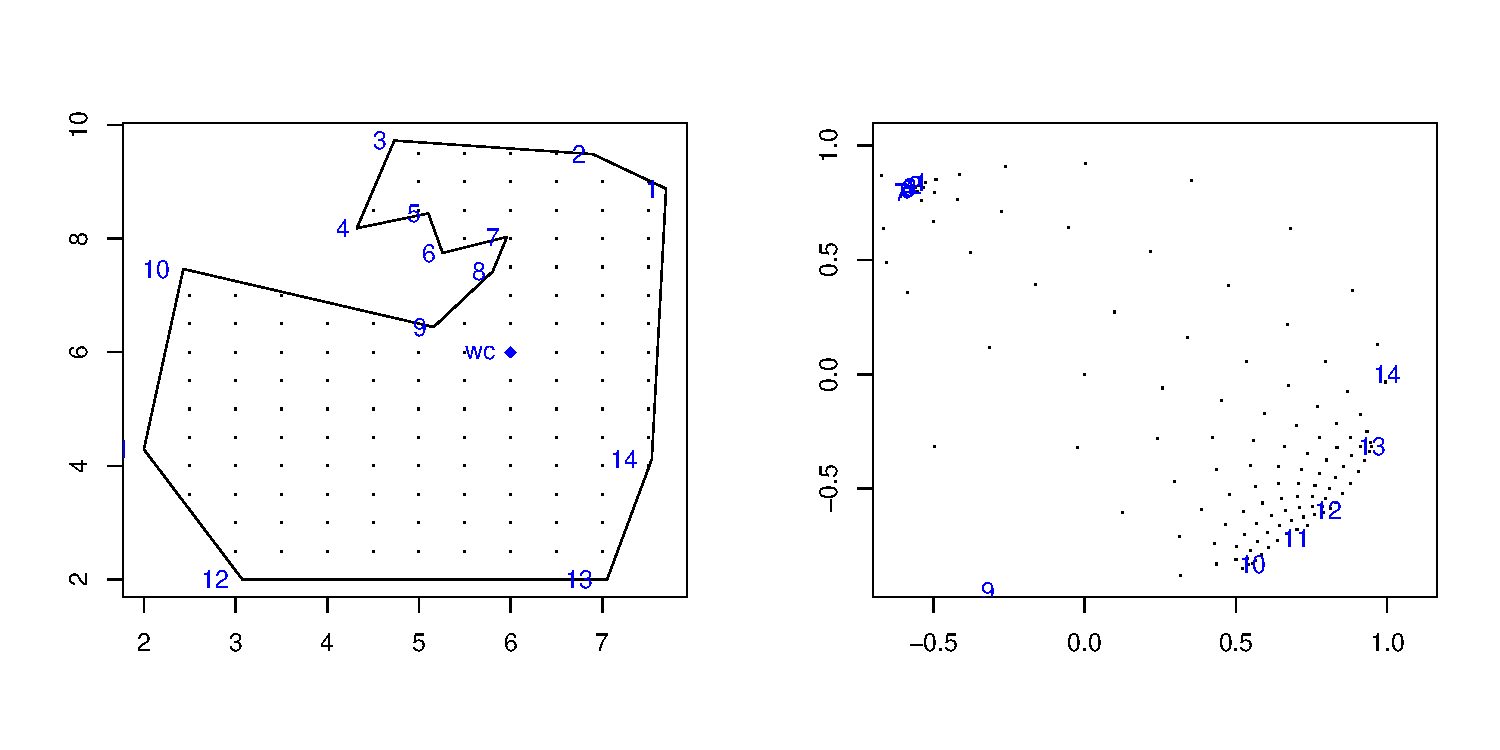
\includegraphics[scale=0.5]{sc/figs/crowdeddisk.pdf}
\caption{An example of crowding. Note that prevertices 1 through 8 are mapped almost to a singularity in the right panel.}
\label{crowdeddisk}
\end{figure}

\subsubsection{Fixing crowding}

If the crowding is caused by $\Gamma$ being elongated then a  primitive fix is to map to an elongated domain such as the rectangle or plane. This approach is suggested in \cite{howell90} however, as they point out, this does not eliminate all crowding and problems can still occur when there are strongly acute peninsulae in the polygon. Mapping to an elongated domain also does not fix problems which occur when mapping from T- or H-shaped domains (so-called ``multiply elongated'' domains).

In order to combat this problem more effectively, \cite{vavasis96} propose the CRDT (cross-ratios of the Delaunay triangulation) algorithm (see below). Each set of prevertices has $n-3$ degrees of freedom hence, there is a three parameter family of possible vertex arrangements that all map to the same polygon. The most stable of these \emph{embeddings} should be used. The M\"{o}bius transformation relates the embeddings to one another.

This idea can be extended by noting that the polygon is identical when additional vertices are added between the current ones, provided that the internal angle associated with the new vertex is $\pi$. These extra vertices also do not change the \sch formula since in \eqn{unitscmap} $\alpha_k=1$ for an angle of $\pi$. Adding these extra vertices allows us to control the aspect ratio of the mapping.

In the solution to the \sch parameter problem given in \secref{sc-parprob}, conditions on the side lengths and orientations of the polygon are enforced. The CRDT algorithm imposes conditions about quadrilateral sections of the polygon and the diagonals of the polygon. First a Delaunay triangulation of the domain is performed and then pairs of triangles are merged into quadrilaterals. A measure is then defined (the \emph{cross-ratio}) which specifies a set of non-linear equations to be solved. These equations enforce the constraint that the cross-ratio in mapped polygon comes out correctly. 

Putting all of these ideas together gives the CRDT algorithm (\cite{driscoll}, pp. 30-39). We first add edges to the polygon with internal angle $\pi$ to remove enlongated parts of the domain and then triangulate the domain. Once the domain is triangulated we find the cross-ratio:
\begin{equation}
\rho(a,b,c,d) = \frac{(d-a)(b-c)}{(c-d)(a-b)},
\end{equation}
for each of the $n-3$ quadrilaterals in the polygon (where $a,b,c,d$ are prevertices). Then, analogously to \eqn{optimizeme} we set up a series of equations, specifying that the cross-ratios remain the same in the polygon and the transform of the rectangle back to the polygon. We then wish to solve for the values of $\rho$ for the original domain in the same manner as we solved for side lengths in the original problem. 

In \fig{uncrowdeddisk} the CRDT method is used with a rectangular domain, crowding has been alleviated to some degree. The point density, as well as vertex density seems to be more uniform than in \fig{crowdeddisk}.

% Uncrowded mapping diagram
\begin{figure} [tbp]
\centering
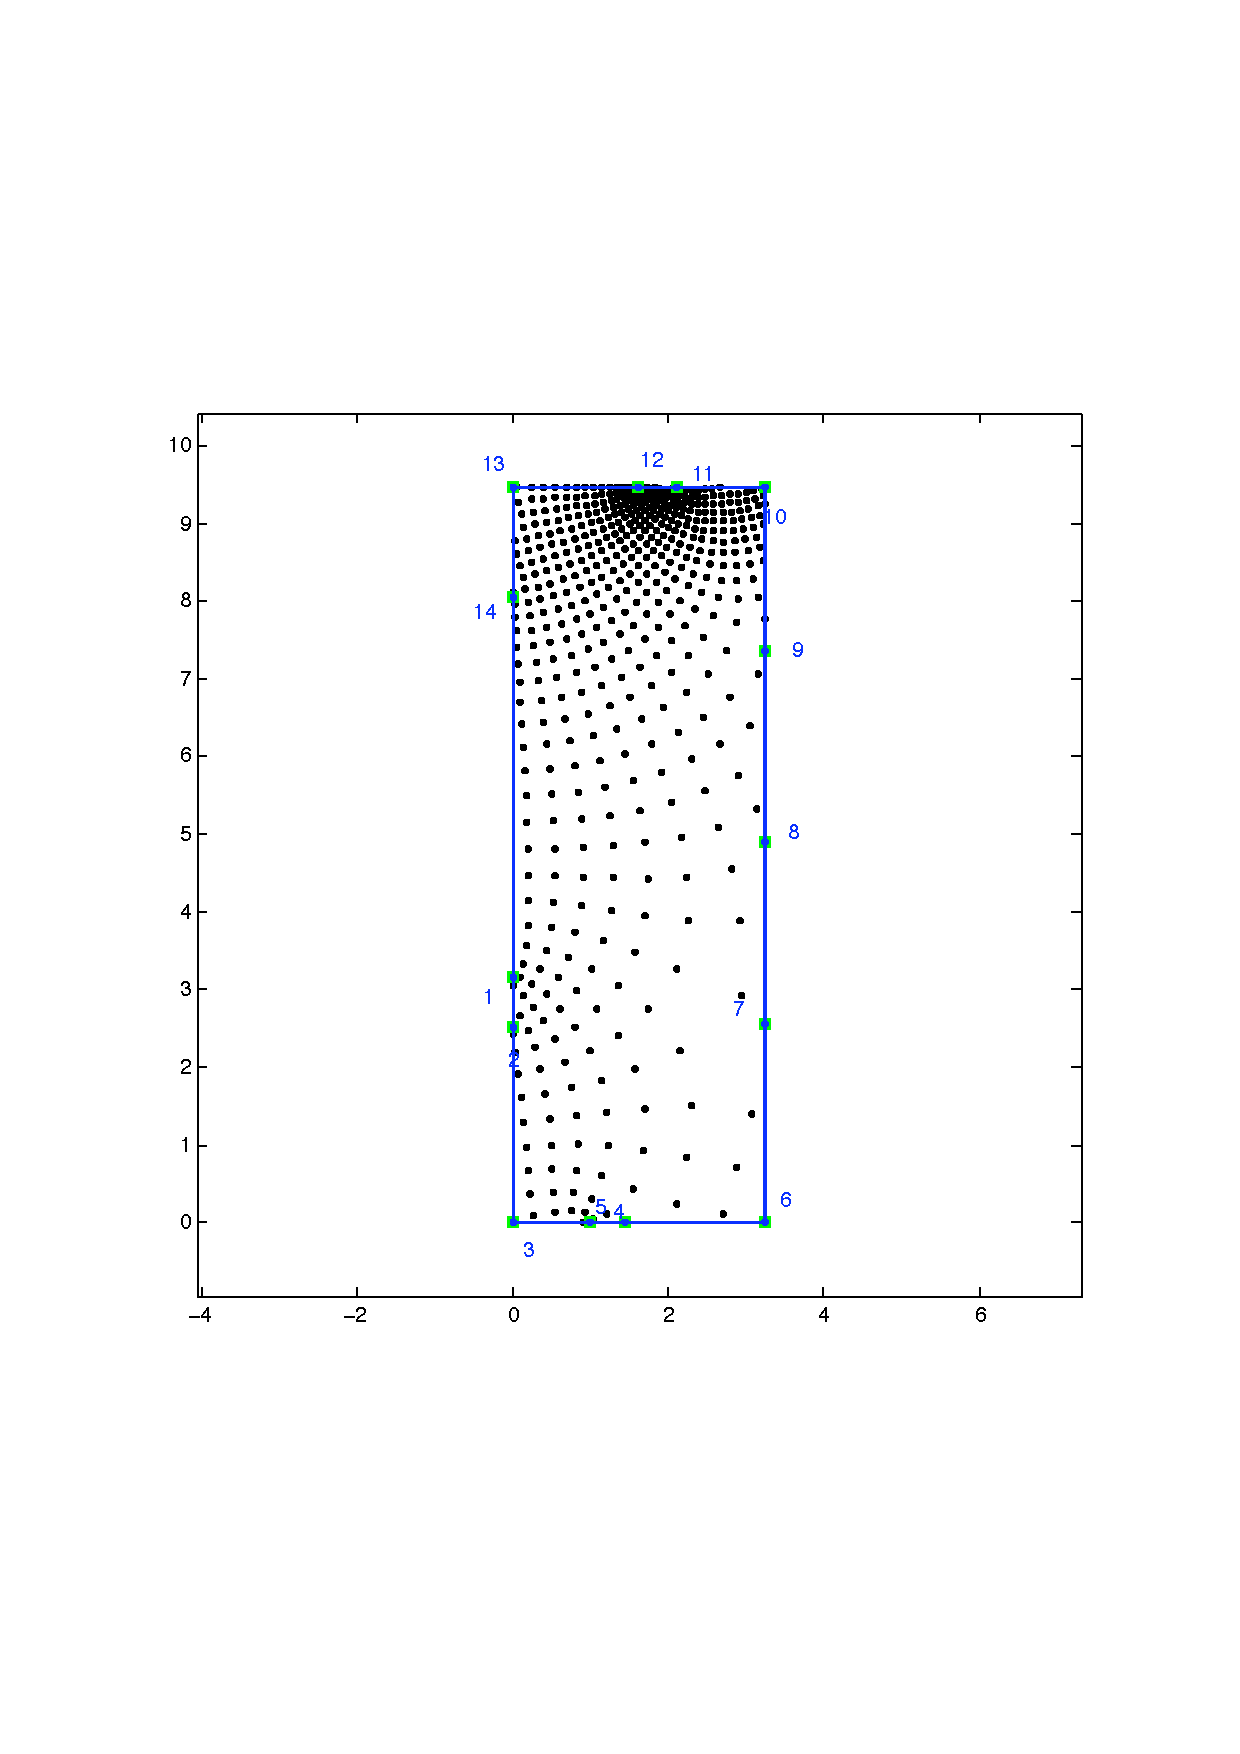
\includegraphics[scale=0.5]{sc/figs/irregular-fixed-crdt.pdf}
\caption{The mapping of the irregular domain featured in \fig{crowdeddisk} using the CRDT method mapping to a rectangle. The crowding is now much less severe.}
\label{uncrowdeddisk}
\end{figure}

The downside of using CRDT is that it may add too many vertices to maintain the aspect ratio, so the algorithm takes longer to run than the one specified in \secref{algorithmsketch} since it tends to be cubic in the number of vertices (\cite{driscoll05}). This is offset against the fact that the problem becomes tractable.

\section{Simulation experiments}

In order to test the efficacy of the \sch transform for the purposes of smoothing over complex regions, a series of simulation experiments were performed. The \emph{SC Toolbox} for MATLAB was used to perform the transform and the mapping of the points. These were then fed into \textsf{R} and models run using packages \texttt{mgcv} and \texttt{soap}.

\subsection{Ramsay horseshoe}

The most obvious candidate for simulation is the Ramsay horseshoe (see \secref{ramsayfunc}). In order to map the horseshoe, we first draw a rough bounding box around the shape. In order to map as simple a domain as possible, to begin with a bounding box was used as the $W$ domain remapped via the \texttt{evalinv()} function from the \emph{SC Toolbox}. This is shown in \fig{hswithboundingbox}. The bounding box is then transformed to the rectangle. 

\begin{figure}
\centering
% trim order l b r t
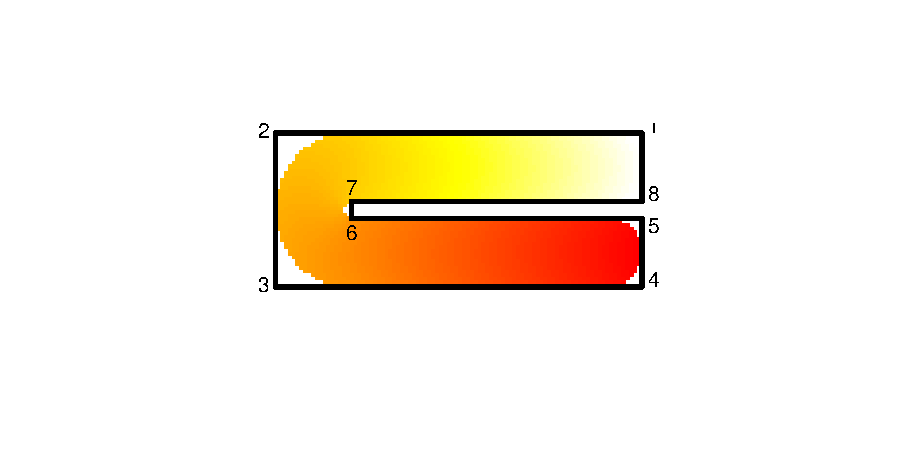
\includegraphics[trim=0.5in 1in 0in 0.5in]{sc/figs/hswithboundingbox.pdf} \\
\caption{The horseshoe with its bounding box. The vertices marked 1, 4, 5 and 8 are mapped to the corners of the rectangle.}
\label{hswithboundingbox}
% generated by /phd-smoothing/sc-writeup/figs/hswithboundingbox.R
\end{figure}

A sample of 1000 points was then taken from the horseshoe and noise added to the data. First the $x$,$y$ coordinates of the sampled points were expressed as complex numbers of the form $w=x+iy$. The sample was then mapped into $W^*$, creating a new set of coordinates $w^*=x^*+iy^*$. Smoothing was then performed over the responses in the $W^*$ domain using the \texttt{gam()} function in \texttt{mgcv}. 

\begin{figure}
\centering
% trim order l b r t
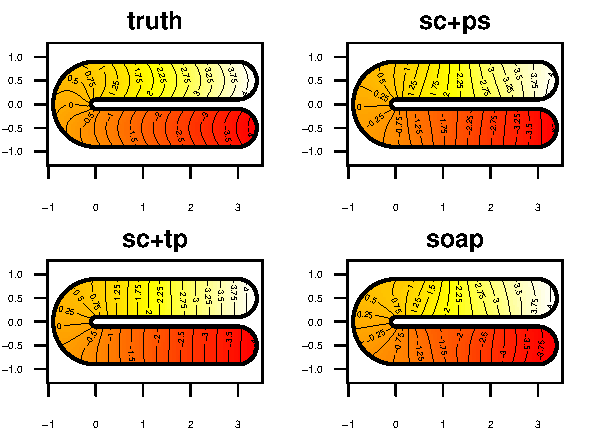
\includegraphics[width=4in]{sc/figs/compsmooth.pdf} \\
\caption{A typical set of predictions using P-splines on the transformed domain (top right), thin plate splines on the transformed domain (bottom left) and soap film smoother (bottom right) for the Ramsay horseshoe (top left). Sample size was 250, noise level was set to $\sigma=1$.}
\label{compsmooth}
% generated by figs/pspline.soap.comp.hs.R
\end{figure}

\Fig{compsmooth} shows the true function and typical realisations of: the fit given by a \tprs on the transformed domain, a P-spline fit on the transformed domain and the fit given by the soap film smoother. Looking at the heat maps one can see that the general shape of the horseshoe function is clearly being reproduced by all methods (especially in comparison to that in \fig{leakage}). However, on the transformed domains the curvature across the minor axis is not being captured.

\begin{table}[tb]
\begin{tabular}{c c}\\
Sample size & Noise level \\
\hline
\hline
1000 & 0.3 \\
500 & 0.3 \\
250 & 0.3 \\
100 & 0.3 \\
1000 & 0.5 \\
1000 & 1 \\
1000 & 2 \\
\end{tabular}
\caption{Setup for the simulations using the \sch transform for the Ramsay horseshoe. Noise level ($\sigma$) is the number a random deviate from a standard Normal distribution was multiplied by before being added to the true test function.}
\label{scramsimtable}
\end{table}

\Tabref{scramsimtable} shows the settings for noise level and sample size of the simulations. Mean squared error between the true function and the fitted model was used to evaluate the performance of the models. In the following tables we provide the mean squared error over a prediction grid of 1000 points averaged over 1000 generated data sets. The fits on the transformed domain and the soap film have much smaller MSE than the thin plate spline, except in one case, \sch with P-splines for sample size 100 and noise level 0.3. Looking closer at the results for this model, there were two results where the MSE was 54.68 and 437.99 which, when removed, put the MSE back to 0.03003, which seems much more reasonable. These results were presumably due to the P-splines having the same knot setup for each realisation, giving a poor model when there was not enough data. This shows one of the many disadvantages of a knot-based approach.

\begin{figure}
\centering
% trim order l b r t
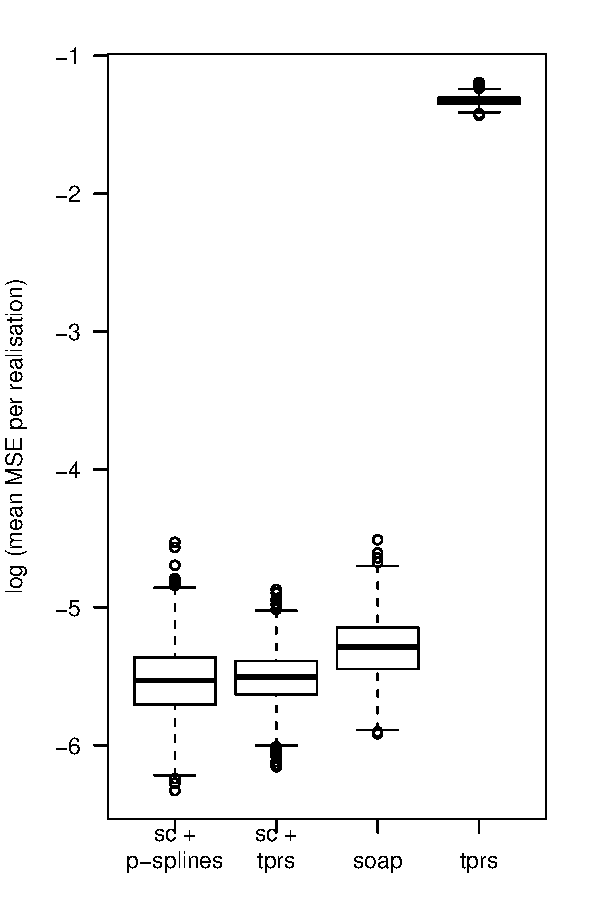
\includegraphics{sc/figs/sc-mses-boxplot.pdf} \\
\caption{Boxplots of mean MSE from 1000 points on a prediction grid from 1000 simulations for the Ramsay horseshoe. Models fitted were \sch transform with P-splines and \tprs, the soap film smoother, and \tprs (with the untransformed domain). Error level was set to 0.3.}
\label{scram1000boxplots}
% generated by sc/figs/makeboxplots.R
\end{figure}

\begin{table}[ht]
\begin{tabular}{c c c c c c}\\
& & & MSE (se) &\\
Sample size & Noise level & TPRS & SC + P-spline& SC + TPRS & Soap film\\
\hline
\hline
%1000 & 0.3 & 0.00412 (0.00112) & 0.00811 (0.00243) & 0.00517 (0.00114) \\ 
%500 & 0.3 & 0.00505 (0.00144) & 0.00478 (0.000955) & 0.00628 (0.00146) \\ 
%250 & 0.3 & 0.00875 (0.00392) & 0.00684 (0.00183) & 0.0107 (0.00305) \\ 
%100 & 0.3 & 0.0225 (0.035) & 0.0118 (0.00461) & 0.0219 (0.0117) \\ 
%1000 & 0.5 & 0.0105 (0.00353) & 0.00811 (0.00243) & 0.0127 (0.0034) \\ 
%1000 & 1 & 0.0242 (0.0108) & 0.0161 (0.0069) & 0.0275 (0.00958) \\ 
%1000 & 2 & 0.066 (0.0481) & 0.0388 (0.0229) & 0.0686 (0.0333) \\ 
1000 & 0.3 & 0.26611 (0.00029) & 0.00412 (4x10$^{-5}$) & 0.00811 (8x10$^{-5}$) & 0.00517 (4x10$^{-5}$) \\ 
500 & 0.3 & 0.28276 (0.00083) & 0.00505 (6x10$^{-5}$) & 0.00478 (4x10$^{-5}$) & 0.00628 (7x10$^{-5}$) \\ 
250 & 0.3 & 0.32274 (0.00268) & 0.00875 (0.00025) & 0.00684 (0.00012) & 0.01073 (0.00019) \\ 
100 & 0.3 & 0.48371 (0.01765) & 0.52264 (1.39562) & 0.01178 (0.00046) & 0.02194 (0.00117) \\ 
1000 & 0.5 & 0.27336 (0.00032) & 0.01055 (0.00011) & 0.00811 (8x10$^{-5}$) & 0.01268 (0.00011) \\ 
1000 & 1 & 0.30718 (0.00056) & 0.02422 (0.00034) & 0.01607 (0.00022) & 0.02749 (3x10$^{-4}$) \\ 
1000 & 2 & 0.42296 (0.00144) & 0.06596 (0.00152) & 0.03875 (0.00072) & 0.06859 (0.00105) \\ 
\end{tabular}
\label{scramsayres}
\caption{Mean squared error along with its standard error for the transformed Ramsay horseshoe (for P-spline and thin plate cases) versus those for the soap film smoother. See below for information on the asterisked result.}
% generated by /phd-smoothing/sc-writeup/tablecode/ramsay.sim.results.table.R
\end{table}

\Tabref{scramsayres} shows the results from the simulations for the horseshoe. The \sch transform yields results which are comparable, it not better, than the soap film. Once we get to 100 samples the method performance degrades over all methods. Although this seems initially encouraging, it is worth bearing in mind at this point that in domains like the horseshoe it is obvious what the transform should be.

Indeed, this can be seen by looking at the predicted values for the model in the $W^*$ domain. \Fig{hsvisgam} shows predictions from the fitted surface alongside the true values when the domain has been put into its ``natural'' coordinate system. The coordinate system for the fitted values is the \sch transformed system and for the true values the system is the major and minor axes of the shape (ie. one axis along the central curve of the shape and the other perpendicular to that). In the plot, the strong linear trend along the major axis of the horseshoe can be seen in both cases, making this a rather trivial smoothing problem. The smooth is being calculated in a close approximation to its natural domain. Such an approximation would not be as easy to find for a less regular, more realistic domain.

\begin{figure}
\centering
% trim order l b r t
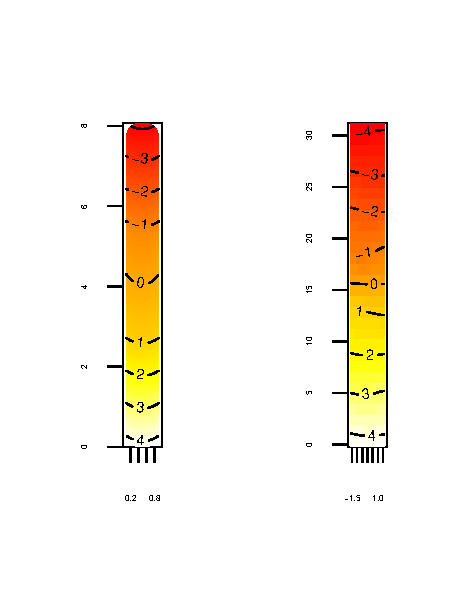
\includegraphics[trim=0in 0.5in 0in 0in]{sc/figs/hsvisgam.pdf} \\
\caption{Heatmap of the true values of the modified Ramsay horseshoe projected into its natural domain (left) and the predicted values of the fit given using the \sch transform and then smoothed using a \tprs (right).}
\label{hsvisgam}
% generated by /phd-smoothing/thesis/sc/figs/hsvisgam.R
\end{figure}

\subsubsection{Alternate Ramsay horseshoe}

The second domain tested was the alternate version of the Ramsay horseshoe from \cite{soap}. For this domain the gradient runs across the short axis of the horseshoe (see \fig{altramsayhorseshoe}). The same simulation setup was used as for the first domain.

\begin{figure}
\centering
% trim order l b r t

\includegraphics[trim=0.5in 1in 0in 0.5in]{sc/figs/altramsayhorseshoe.pdf} \\
\caption{Heatmap of the alternate version of the Ramsay horseshoe.}
\label{altramsayhorseshoe}
\end{figure}

For the alternative horseshoe we begin to see the soap film creep ahead of the transformation method (see \tabref{scaltramsayresultstable}). Although the MSEs are of approximately the same order (as are the standard errors), the soap film is gaining ground. 


To examine what is going on here we can look at the plots of the predicted values as heat maps. These can be seen in \fig{altramsaycomp} and show that the \sch mapping seems to capture the overall structure of the shape better than the soap film smoother, which seems to capture patches of the shape but not the overall structure. It also appears that the \sch method does not respect the ends of the horseshoe and continues the gradient running along the minor axis over this part as well.This feature seems to be the cause of the performance decrease.

------------------------


\begin{table}[ht]
\begin{tabular}{c c c c c c}\\
& & & MSE (se) &\\
Sample size & Noise level & TPRS & SC + P-spline& SC + TPRS & Soap film\\
\hline
\hline
%1000 & 0.3 & 0.00415 (0.00117) & 0.0158 (0.00247) & 0.00378 (0.00108) \\ 
%500 & 0.3 & 0.00469 (0.00147) & 0.00793 (0.00186) & 0.00458 (0.00145) \\ 
%250 & 0.3 & 0.00716 (0.00431) & 0.0142 (0.00249) & 0.00771 (0.00301) \\ 
%100 & 0.3 & 0.039 (0.22) & 0.0201 (0.00589) & 0.0298 (0.42) \\ 
%1000 & 0.5 & 0.00839 (0.00403) & 0.0158 (0.00247) & 0.00966 (0.00371) \\ 
%1000 & 1 & 0.0194 (0.0122) & 0.0226 (0.0085) & 0.019 (0.00981) \\ 
%1000 & 2 & 0.0605 (0.0468) & 0.0436 (0.0276) & 0.041 (0.0434) \\ 
1000 & 0.3 & 0.0109 (8x10$^{-5}$) & 0.00415 (4x10$^{-5}$) & 0.01579 (8x10$^{-5}$) & 0.00378 (3x10$^{-5}$) \\ 
500 & 0.3 & 0.01395 (1x10$^{-4}$) & 0.00469 (7x10$^{-5}$) & 0.00793 (8x10$^{-5}$) & 0.00458 (6x10$^{-5}$) \\ 
250 & 0.3 & 0.01721 (2x10$^{-4}$) & 0.00716 (0.00027) & 0.01418 (0.00016) & 0.00771 (0.00019) \\ 
100 & 0.3 & 0.0229 (0.00099) & 0.03904 (0.02197) & 0.02011 (0.00059) & 0.02975 (0.04195) \\ 
1000 & 0.5 & 0.01521 (6x10$^{-5}$) & 0.00839 (0.00013) & 0.01579 (8x10$^{-5}$) & 0.00966 (0.00012) \\ 
1000 & 1 & 0.02084 (0.00023) & 0.01943 (0.00038) & 0.02264 (0.00027) & 0.01902 (0.00031) \\ 
1000 & 2 & 0.03843 (0.00072) & 0.06053 (0.00148) & 0.04363 (0.00087) & 0.04096 (0.00137) \\ 
\end{tabular}
\label{scaltramsayresultstable}
\caption{Mean squared error along with its standard deviation for the transformed alternate Ramsay horseshoe (for P-spline and thin plate cases) versus those for the soap film smoother.}
% generated by /phd-smoothing/sc-writeup/tablecode/alt.ramsay.sim.results.table.R
\end{table}

\begin{figure}
\centering
% trim order l b r t
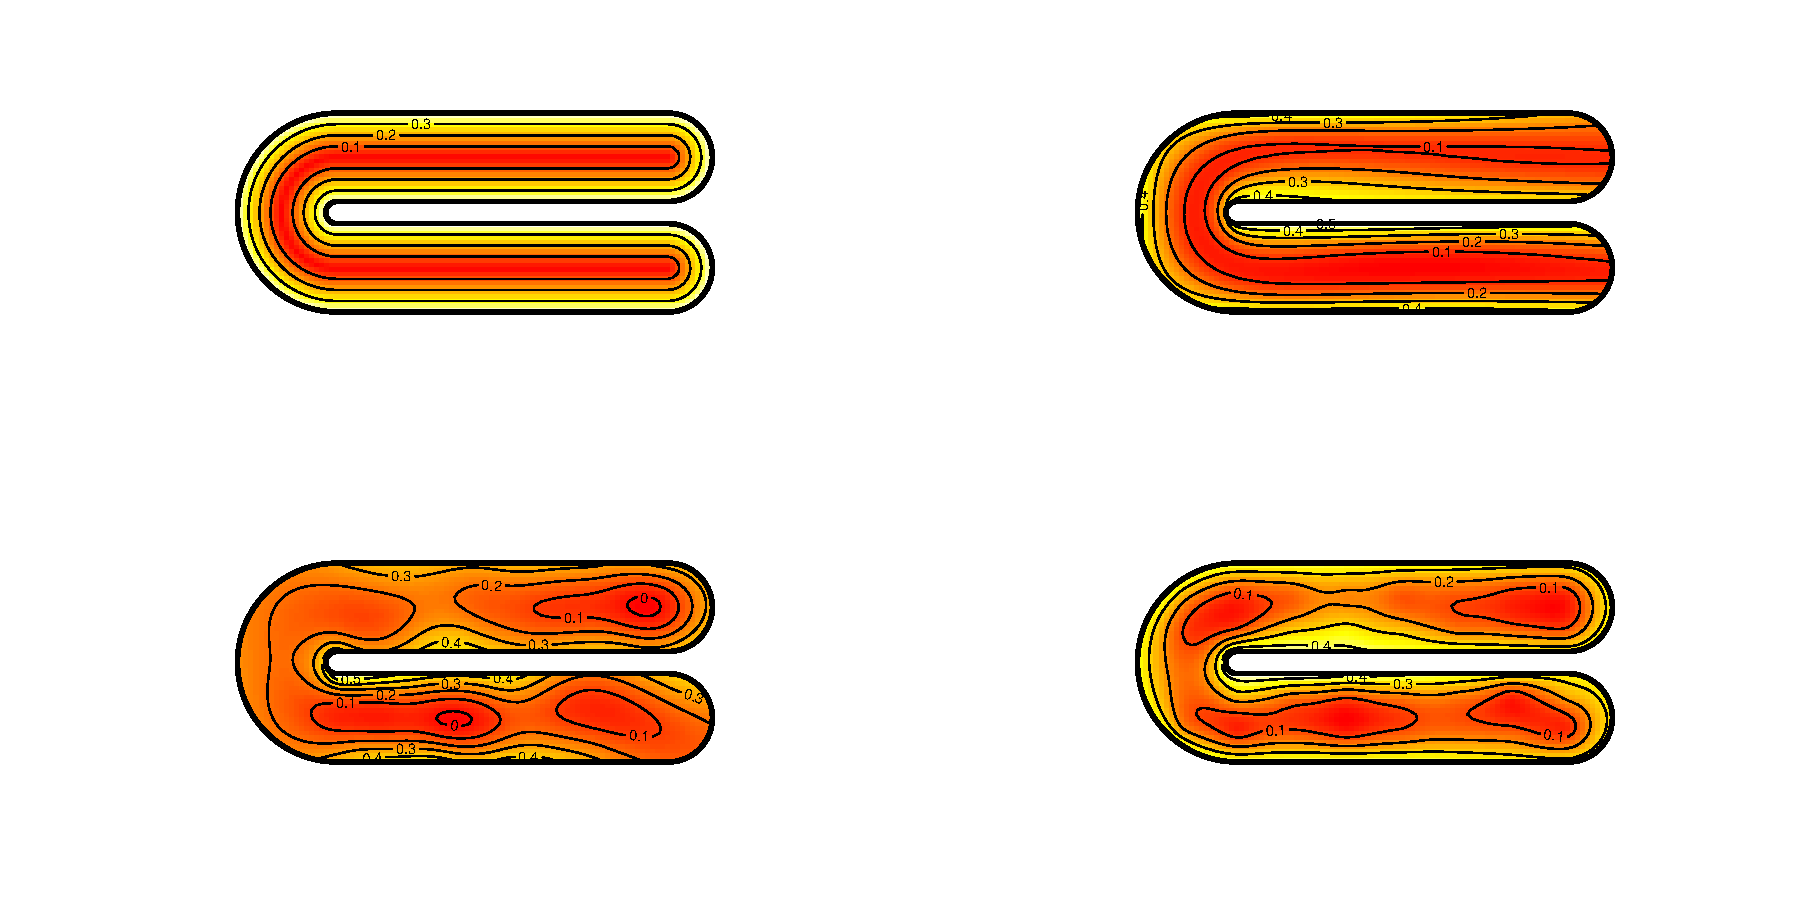
\includegraphics[width=4in]{sc/figs/altramsaycomp.pdf}\\
\caption{Single realisations of the fit to the alternate Ramsay horseshoe for each method. Clockwise from top left: the original figure, the function estimated by the \sch transform with P-splines, function estimated by the \sch transform with thin plate splines and finally the soap film estimate. Error set to $\sigma=1$.}
\label{altramsaycomp}
% generated by /phd-smoothing/sc-writeup/figs/altramsaycompare.R 
\end{figure}


\subsubsection{What's happening?}

At this point it is useful to get an idea about what the transformation is doing to the domain, specifically to find out about the distortion to space caused by the transform. To investigate this we can take a straight line in the $W$ domain and see what it maps to in the $W^*$ domain. We can also look at the response along that line according to the transformed and untransformed coordinate systems and see how this compares to looking at the response in the horseshoe's natural coordinate system.

\begin{figure}
\centering
% trim order l b r t
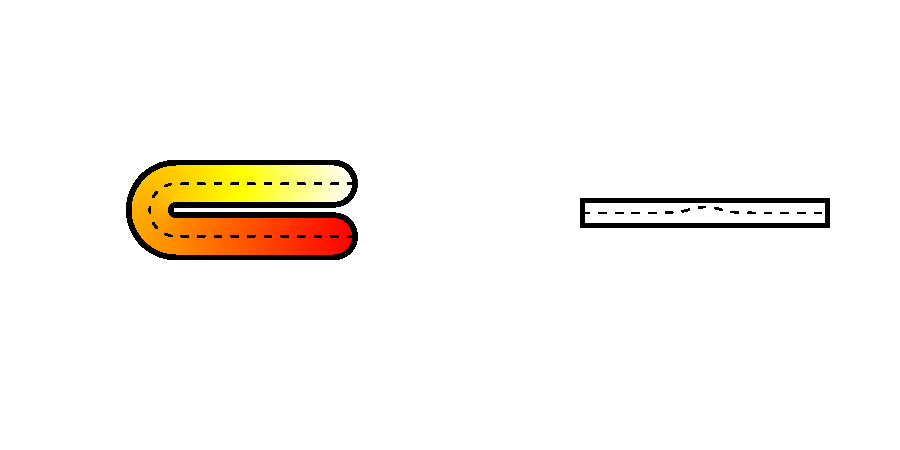
\includegraphics[trim=0.5in 1in 0in 1in]{sc/figs/horseshoecentreline.pdf} \\
\caption{Mapping of a straight line along the major axis of the Ramsay horseshoe to its position in the ``unwrapped'' domain.}
\label{horseshoecentreline}
% generated by /phd-smoothing/ramseysim/nullspace.test.R 
\end{figure}

\Fig{horseshoecentreline} shows the line that was evaluated along the centre of the horseshoe and its equivalent line in the transformed domain. We can see from this that a line that is straight in the domain appears to be bent in the transform. The curvature does not appear to be particularly extreme in this case, however, one can imagine that this could get significantly worse for regions with more complicated boundaries. Although this is interesting, it is more revealing to look at the evaluations of the horseshoe functions along that line.

\Fig{centrelinelineplot} shows the evaluations of the horseshoe function over the line plotted against three coordinate systems. The first plot shows the function evaluations on the $W$ domain as a response to change in $y$. The second on the $W^*$ domain, as a response to $y^*$, in the transformed coordinate system. The final plot is in the horseshoe's ``natural'' domain, \emph{ie.} the value the horseshoe takes as a function of distance along the major axis of the shape. From these plots one can see the quality of approximation to the natural domain of the horseshoe the \sch transform affords. Only two minor kinks occur in the line. Looking at where the kinks occur, they correspond exactly to those kinks in \fig{horseshoecentreline}. This makes sense, since we would expect a change in gradient if direction we are traveling has moved into two dimensions from one.

\begin{figure}
\centering
% trim order l b r t
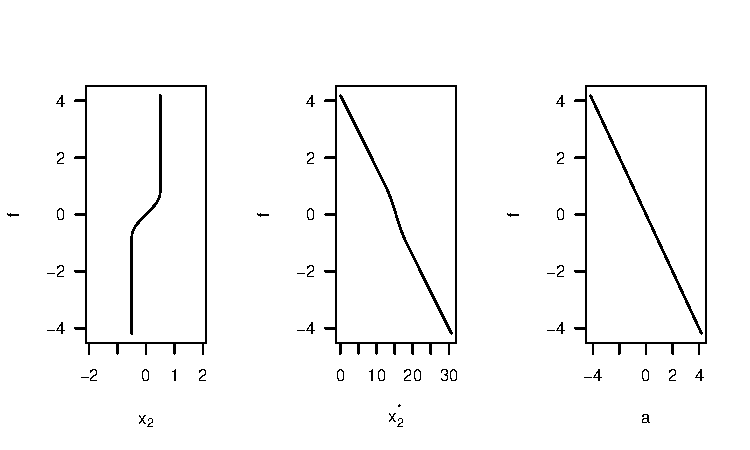
\includegraphics[trim=0in 0in 0in 0in]{sc/figs/centrelinelineplots.pdf} \\
\caption{Plots of the horseshoe function against the $y$ axis for (left) the untransformed horseshoe, (middle) the shape under the \sch transform and, (right) the function evaluation against the major axis.}
\label{centrelinelineplot}
% generated by /phd-smoothing/ramseysim/nullspace.test.R 
\end{figure}


\Fig{altcentrelinelineplot} shows analogous plots to \fig{centrelinelineplot} and backs up this hypothesis. The second panel shows the mapping of the $y$ component of the centreline against the response and the third panel shows the same in the horseshoe's own domain. The two plots appear to be indistinguishable.

\begin{figure}
\centering
% trim order l b r t
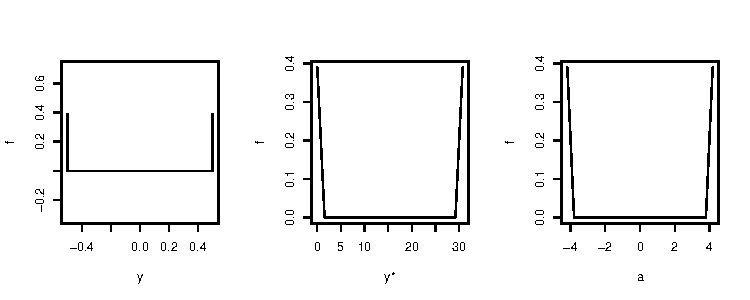
\includegraphics[trim=0in 0in 0in 0in]{sc/figs/altcentrelinelineplots.pdf} \\
\caption{Plots of the alternate horseshoe function against the $y$ axis for (left) the untransformed horseshoe, (middle) the shape under the \sch transform and, (right) the function evaluation against the major axis.}
\label{altcentrelinelineplot}
% generated by /phd-smoothing/altramsaysim/nullspace.test.R 
\end{figure}



\section{Conclusions \& Analysis}

This brief foray into conformal mapping has provided plenty of insights into how smoothers will act under mapping schemes. It also gives insight into which criteria are useful for a transformation-based method. For example, the angle-preserving properties of the \sch transform are of little use in a smoothing context. It is also clear that a method that does not produce crowding-type phenomena is desirable. These examples show the serious disadvantages of the approach, the ability of the transform to clearly split the domain and truly separate those parts interfering with one another is very useful.

Although the \sch transform is rather disappointing in practice, it does show that a mapping-type technique can produce some reliable results, even if it is on a limited number of domains. In essence the main downfall of the \sch transform is that it re-maps the domain too rigidly. There is no flexibility to the domain into which one is mapping, it must be one of those detailed above. It is now clear that such an inflexible strategy will not yield good results in all situations and, indeed, there are a limited number of situations in which such an approach will be useful.



\chapter{Multidimensional scaling for domain-dependent finite area smoothing}

% MDS stuff

\label{chap-mds}

\section{Introduction}

Following the work of the previous chapter, the objective is now to find a mapping of the data into a new space which causes minimum distortion to the points in that new space. At the same time the mapping must also effectively separate those parts of the original domain which are subject to leakage. This balance (between making sure the model overcomes leakage whilst at the same time does not cause artefacts in the smooth) is essential to the success of the approach. The \sch\ transform approach, of dictating the transformed domain from the outset is clearly not flexible enough for general use, however a method that depends on the shape of original domain may have more promise.

\subsection{Proposition}

Multidimensional scaling (MDS) or, as it is often referred to, principle coordinates (PCO) (\cite{gower1966}) is a method used in multivariate analysis. It is closely related to techniques such as PCA (\cite{chatfieldcollins}, p. 200) and canonical correspondence analysis (\cite{terbraak}). The starting point for MDS is a matrix of distances, representing some kind of dissimilarity between observations. This distance could be calculated from the data, for example ideological distance between politicians measured using NOMINATE scores (\cite{quantss}, p. 225), or could instead be distances that occur in the data naturally through experimental setup,  for example comparative distances between stimuli response in a psychophysical experiment (\cite{torgerson}). Here we concentrate on geographical distances.

MDS takes this matrix of distances and projects the data in such a way that Euclidean inter-point distances in the projection are approximately the same as the distances in the matrix (\cite{chatfieldcollins}, p. 187). If the matrix of distances is of rank $m$ then the projection can be in $m-1$ or less dimensions; a projection into 2 dimensions is a typical choice, since it is easily visualised. For this reason one can also think of MDS as a dimension reduction technique, finding a projection of a data cloud into lower dimensional space, while still retaining information about the dissimilarities between the points.

When MDS is performed on some categorised set of dissimilarities (as is often the case in social science and psychology) it is referred to as non-metric MDS, where as on a continuous scale it is known as metric MDS. Though they have different names, the calculations are identical (aside from the method of finding the distances). Discussion here will focus on metric MDS.

Multidimensional scaling offers a framework for finite area smoothing over a region with a complex boundary. Given the set of distances between points in a domain, we can project those points into a configuration such that the distances between those points are approximately preserved. Now, if the Euclidean metric were to be used to calculate the distances between the points then the result from the projection would be identical to the starting point configuration (provided that we projected back into the same number of dimensions). However, if it were possible to use a metric that took into account the distance within the boundary (a within-area distance) then the resulting configuration of points would (approximately) respect the boundary of the domain.

Justification for this approach is as follows. In many applications within-area distances is meaningful, given that there is some reasoning behind why certain parts of the domain should not affect one another. Biological populations respect the intrinsic structure of these domains and in general do not respect Euclidean geometry in their movement patterns (for example, they move around obstacles, avoid predators and track prey). When within-area distances are meaningful, it makes sense to use this information about the structure of the domain rather than somewhat arbitrarily choose Euclidean geometry and discard this extra informaton. However, as literature on smoothing is firmly based in a Euclidean context, it would be preferable to perform the smoothing in Euclidean space. In this case the approximation to Euclidean space afforded by an MDS projection of the within-area distances offers a bridge between these two requirements.

\subsection{Procedure}
\label{mdsproc}
Given a sample $\{\bm{x}_i, z_i : i=1\dots n\}$, the set of points in the domain over which smoothing is to be performed, $\bm{x}_i$ is the location (a $k$-vector, although here 2-vectors are assumed throughout) of the $i^\text{th}$ point with response $z_i$ (assumed to be univariate). Here, finding an MDS configuration of a set of points consists of: $i$) calculating the within-area distances between the points, $ii$) forming the distance matrix and, $iii$) actually performing the MDS projection.

The whole proposed procedure is as follows:

\begin{enumerate}
\item Obtain the MDS configuration for the domain using some representative set of points over the area in question. The only use of the MDS locations obtained in this step is to find the initial MDS configuration; they are discarded afterward. Representative points could be a sparse grid over the domain or a subset of $\{\bm{x}_i : i=1\dots n\}$. More detail and justification is provided in \secref{grids}, below.

\item Using the MDS configuration obtained above along with Gower's interpolation (see \secref{gowers}) to obtain the location of the sample in the MDS configuration: $\{\bm{x}_i^*, z_i : i=1\dots n\}$.

\item Smooth $\{\bm{x}_i^*, z_i : i=1\dots n\}$ using a penalised regression spline.

\item To predict at a location $\bm{x_j}$ in the original domain, use Gower's interpolation to obtain the point's location in the MDS space: $\bm{x}_j^*$. Predict $\hat{z}_j$ at $\bm{x}_j$ using the smooth at $\bm{x}_j^*$.
\end{enumerate}

This approach is referred to as \mdsap\ (MultiDimensional Scaling with Regression Splines) throughout the chapter.

The rest of this chapter is structured as follows: in \secref{MDStechdet} a technical overview of MDS is given, along with technical details of how the MDS configuration is calculated; \secref{mdsdist} focuses on how the within-area distances are found; \secref{mdssims} shows some examples of this method on simulated data. \Secref{MDSimprov} shows some improvements to the initial method and further simulations, \secref{mds-problems} details remaining problems and \secref{mds-prac} gives some notes for practitioners wishing to use \mdsap. Finally, \secref{mds-conc} draws the topic to a conclusion and lays out areas of further work and interest.


\section{Technical details}
\label{MDStechdet}

The basic concept behind MDS as used here is to take the data, calculate their within-area inter-point distances and then find their points in a new coordinate system based on those inter-point distances. Their new positions are determined by finding the eigen-decomposition of the (centred) matrix of distances between points. First a description of the MDS procedure when Euclidean distances are used is given, followed by the justification for the use of the same procedure when using within-area distances. 

\subsection{Finding the new point configuration}

First define $d_{ij}$ as the distance between the points $i$ and $j$. These are used to form a (symmetric) matrix, $D$, with \ijth element $d^2_{ij}$. For the moment let us assume that $D$ is known and $d_{ij}$ is the Euclidean distance between points $i$ and $j$. 

\cite{diaconis08} gives a clear definition of the algorithm (due to \cite{schoenberg35} and \cite{torgerson}) for finding the new locations of points, which is outlined below. Further detail is given in \cite{principlesofMA}, pp. 104-108 and \cite{chatfieldcollins}, pp. 189-200.

First, suppose that the $n$ unknown new locations (in $n$ dimensions) in our MDS configuration are rows of an $n \times n$ matrix, $\tilde{X}^*$. Now let $S=\tilde{X}^{*} \tilde{X}^{*\text{T}} $, so $S$ is a matrix of scalar products of the point vectors, \emph{ie.} the \ijth element of $S$ is:
\begin{equation}
s_{ij} = \bm{x}_i\tr{\bm{x}_j},
\label{selem}
\end{equation}
$S$ is an $(n\cross n)$ matrix. Note that we may only find $\tilde{X}^*$ up to a translation and rotation, so it is assumed that the values in $\tilde{X}^*$ have been centred about the origin.

We now wish to relate $D$ to $S$. First, note that that \ijth element of D is 
\begin{equation}
d_{ij}^2 = (\bm{x}_i-\bm{x}_j)\tr{(\bm{x}_i-\bm{x}_j)} = \bm{x}_i\tr{\bm{x}_i} + \bm{x}_j\tr{\bm{x}_j}  -2 \bm{x}_i\tr{\bm{x}_j}.
\label{dij}
\end{equation}
Using \eqn{selem}, we can re-write \eqn{dij} as
\begin{equation}
D=\bm{s}_\text{diag}\tr{\bm{1}} + \bm{1}\tr{\bm{s}_\text{diag}} -2S.
\label{dijmat}
\end{equation}
where $\bm{1}$ is an $n \cross 1$ vector of 1s and $\bm{s}_\text{diag}$ is the $n \cross 1$ vector of diagonal elements of $S$.

Define:
\begin{equation}
H = I-\frac{1}{n}\bm{1}\tr{\bm{1}},
\end{equation}
where $I$ is the identity matrix, as usual, and $\bm{1}\tr{\bm{1}}$ is an $n \cross n$ matrix of 1s.

By pre- and post-multiplying any matrix by $H$ the matrix is double centred (such that row and column means are 0). Pre- and post-multiplying \eqn{dijmat} by $H$ yields:
\begin{equation}
HDH = -2HSH.
\end{equation}
The first two terms in on the right hand side of \eqn{dijmat} are zero since the rows of $\bm{s}_\text{diag}\tr{\bm{1}}$ and the columns of  $\bm{1}\tr{\bm{s}_\text{diag}}$ are constant. Since $S$ is already centred so $HSH=S$. Rearranging, the following relation between $S$ and $D$ holds:
\begin{equation}
S = -\frac{1}{2}HDH.
\end{equation}

Now there is a relation between $D$ and $S$, we can concentrate on dealing with $S$. In order to find $\tilde{X}^{*}$ we must factor $S$. There are many options for matrix decomposition. One option for factoring $S$ is to use the Cholesky decomposition, however, with MDS we are looking to decompose the space based on the directions of largest variation, \emph{ie.} those that have the largest contribution to $s_{ij}$. For that reason we use the eigen-decomposition.

Finding the eigen-decomposition of $S$, we obtain $S=U\Lambda\tr{U}$. Here $U$ is the $n \cross n$ orthogonal matrix of eigenvectors and $\Lambda$ is the $n \cross n$ diagonal matrix of eigenvalues. Then an $\tilde{X}^*$ satisfying \eqn{selem} may be computed as:
\begin{equation}
\tilde{X}^*=U\Lambda^{\frac{1}{2}}.
\end{equation}

Following these steps $\tilde{X}^*$ is an $n \cross n$ matrix. The aim here is to smooth in two dimensions, and in general multidimensional scaling is performed to reduce the dimensionality of the data, so we must now reduce the dimensionality of $\tilde{X}^*$. To represent the space using two dimensions the directions with the two largest eigenvalues are chosen and the others discarded. These two largest eigenvalues and their associated eigenvectors constitute the two largest sources of variation in distance (since they are the two largest contributions to $S$) this gives the two dimensional representation of the data. 

Defining $X^*$ to be the $n \cross 2$ dimensional matrix obtained from truncating the full new coordinate set to the first two columns in decreasing eigenvalue order, a 2-dimensional representation has been obtained. More generally, we can find the $k$-dimensional MDS representation of the space by just taking the first $k$ columns of $\tilde{X}^*$.

In summary, to calculate the MDS configuration of a set of points (given their inter-point distances) we merely need to double centre the matrix of distances, perform an eigen-decomposition on the resulting matrix, and finally truncate that matrix to the first $k$ columns.

For finite area smoothing, $d_{ij}$ should be the shortest distance between the points, given the path between any pair of points remains within the domain. Calculation of the inter-point distances is covered in \secref{mdsdist}, however it is important to first justify the use of these steps when non-Euclidean distances are used. 

One can think of the justification in the following way: given that the distances in $D$ obey the triangle inequality, all of the points in $D$ ($n$ of them if $D$ is $n \cross n$) may be represented by MDS in $n$ dimensional Euclidean space (at worst). Hence, in the case where the $d_{ij}$ are Euclidean distances in 2 dimensions, the smallest dimensional space in which they can be represented is 2, but they may still reside in $n$-dimensional space with no loss of information about the distances. So, in the case when the distances in $D$ are shortest within-area distances, one can think of the points in $D$ as residing in a higher number of dimensions in such a way that the distances between them are Euclidean.

Note that an additive constant can be computed and added to the non-diagonal entries of $D$ to ensure that the eigenvalues of $S$ are non-negative. However, this does not occur in any of the examples shown here.

\subsection{Gower's interpolation} 
\label{gowers}
Given the setup in \secref{mdsproc}, once the MDS configuration has been found further points will need to be inserted into our MDS representation. For example when further data is collected, or in order to predict over points not in the initial grid. In this case we would like to insert those new points into the configuration given by MDS. A number of methods have been developed over the past 40 years; Gower's interpolation (\cite{gower1968}) is covered here.

Say we have some point, $x_{\text{new}}$ and we wish to find its location, $x^*_{\text{new}}$ in the MDS configuration. The position of $x^*_{\text{new}}$ is at a Euclidean distance from the points in $X^*$ which is approximately the same as the within-area distance between $x_{\text{new}}$ and the points in the non-transformed space, $X$. 

Note that here we are assuming that a 2 dimensional projection has been used in the initial MDS configuration, Gower's interpolation remains valid for the case in which the initial MDS projection is $k$-dimensional.

\subsubsection{Gower's interpolation formula}

We may find the position in the transformed space, $x^*_{\text{new}}$ , of some new datum $x_{\text{new}}$ in the original space using:
\begin{equation}
x^*_{\text{new}} = \frac{1}{2} \Lambda^{-1} \tr{(X^*)} \mathbb{D}.
\label{gower}
\end{equation}
Here $\Lambda$ ($2 \cross 2$) and $\tr{(X^*)}$ ($2 \cross n$) are as above, $\mathbb{D}$ ($n \cross 1$) is the vector of centred within-area distances from the points in the original configuration to $x_{\text{new}}$.

% Thesis fact: this paragraph infact represents about 3 months of work :(
In Gower's paper, he defines the $i^\text{th}$ element of $\mathbb{D}$ as $-(d^2_{i,\text{new}}-\text{diag}(\tilde{X}^* \tilde{X}^{*\text{T}})_{ii})$, with $d^2_{i,\text{new}}$ being the squared distance from the $i^\text{th}$ point to the new point. The centring is given by the diagonal elements of $\tilde{X}^*\tilde{X^{* \text{T}}}$ \emph{ie}. the squared distances from the original points to the centroid of the MDS configuration. To avoid confusion (and to emphasise that the full $\tilde{X}^*$ matrix is used, rather than its truncated version), it may be easier to think of the expression for the $i^\text{th}$ element of $\bm{d}$ as:
\begin{equation}
d_{i} = -(d^2_{i,n+1}-\text{diag}(S)_{ii}).
\end{equation}
Since $S$ is already known, this expression is more sensible to use for computation as it doesn't imply any extra matrix multiplication.

Gower's interpolation extends simply to the case when $m$ new points are inserted by making $x^*_{\text{new}}$ as $2 \cross m$ matrix and $\mathbb{D}$ an $n \cross m$ matrix.


\subsection{Practical considerations}

Gower's paper shows that performing MDS on a dataset is equivalent to performing MDS on a reduced set of points and then inserting the remaining points, when the Euclidean metric is used to calculate the distances between the points. Extensive testing on a number of different domains has confirmed this.

Before performing any analysis we must test that the method will be reliable and that the mapping that MDS produces is smooth (in terms of the spatial coordinates that it produces). I first motivate the need for using a grid as a start point for the MDS configuration, and then show that the mapping produces smooth lines when within-area distances are used.

\subsubsection{Using grids as a starting point}
\label{grids}
Given that both the finding of the MDS configuration of the points and Gower's insertion rely on the eigenvalues of the original MDS configuration, obtaining representative eigenvalues is important. If those points used to create the initial MDS configuration are not representative of the whole domain, the eigenvalues and eigenvectors may fail to represent the space correctly and, as such, the new point(s) may be inserted incorrectly. This could happen if the initial MDS configuration is created using only points from one half of the domain or, more pathologically, there were a very uneven distribution of points within the domain, in this case only a portion of the full information about the domain would be included in the model. This would lead to the unrepresentative eigenvalues being calculated. Indeed, Gower points this out at the end of his 1968 paper.

When Euclidean distances are used to calculate $D$ the eigenvalues are found correctly given that there is one more point than there are dimensions in the space, provided that the points are not collinear (\cite{landmark}). However, it is not clear what a similar criteria would be for the shortest paths used here. 

A simple example of this problem is show in \fig{tshape}. Here, a regular grid has been generated inside a T -shape (top left panel). The point configuration found by using the full set of points and within-area distances is given in the top right panel. In the pathological case when either only the ``head'' or ``tail'' of the T are sampled and used to generate the MDS and the other half inserted (bottom left for head (red) inserted from tail (black), bottom right of tail (red) inserted from head (black)), one can see that those points inserted into the configuration become warped. 

% showing the the grid is necessary using the T shape
\begin{figure}
\centering
% trim order l b r t
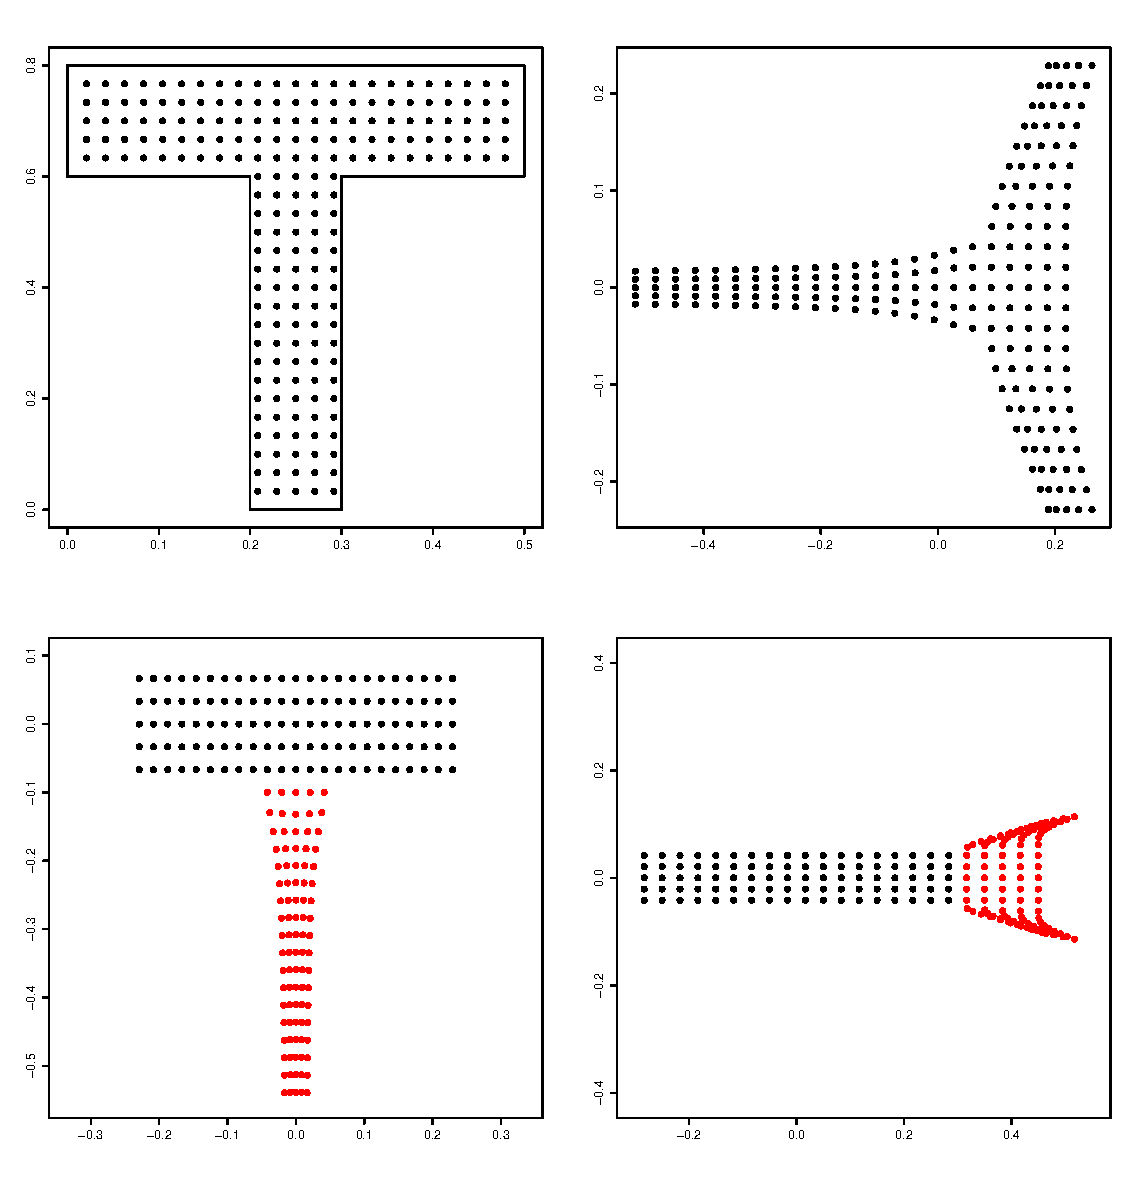
\includegraphics[width=3.5in]{mds/figs/tshape.pdf} \\
\caption{Data generated inside a T-shape (top left) is fed into MDS at once (top right). When either the head or tail of the T is used for the original MDS configuration and the other points inserted, the shape produced is distorted.}
\label{tshape}
% generated using figs/gridtest.R
\end{figure}

Although the cases show in \fig{tshape} are somewhat pathological, looking at more reasonable situations still leads to wildly different results. In \fig{tshaperand} the black and green points make up the original MDS configuration; the five green points are chosen at random. The red points are then inserted. As can be seen in these four typical realisations, the shape of the MDS space is dependent on those points used to create the initial MDS configuration.

% showing the the grid is necessary using the T shape (random samples
\begin{figure}
\centering
% trim order l b r t
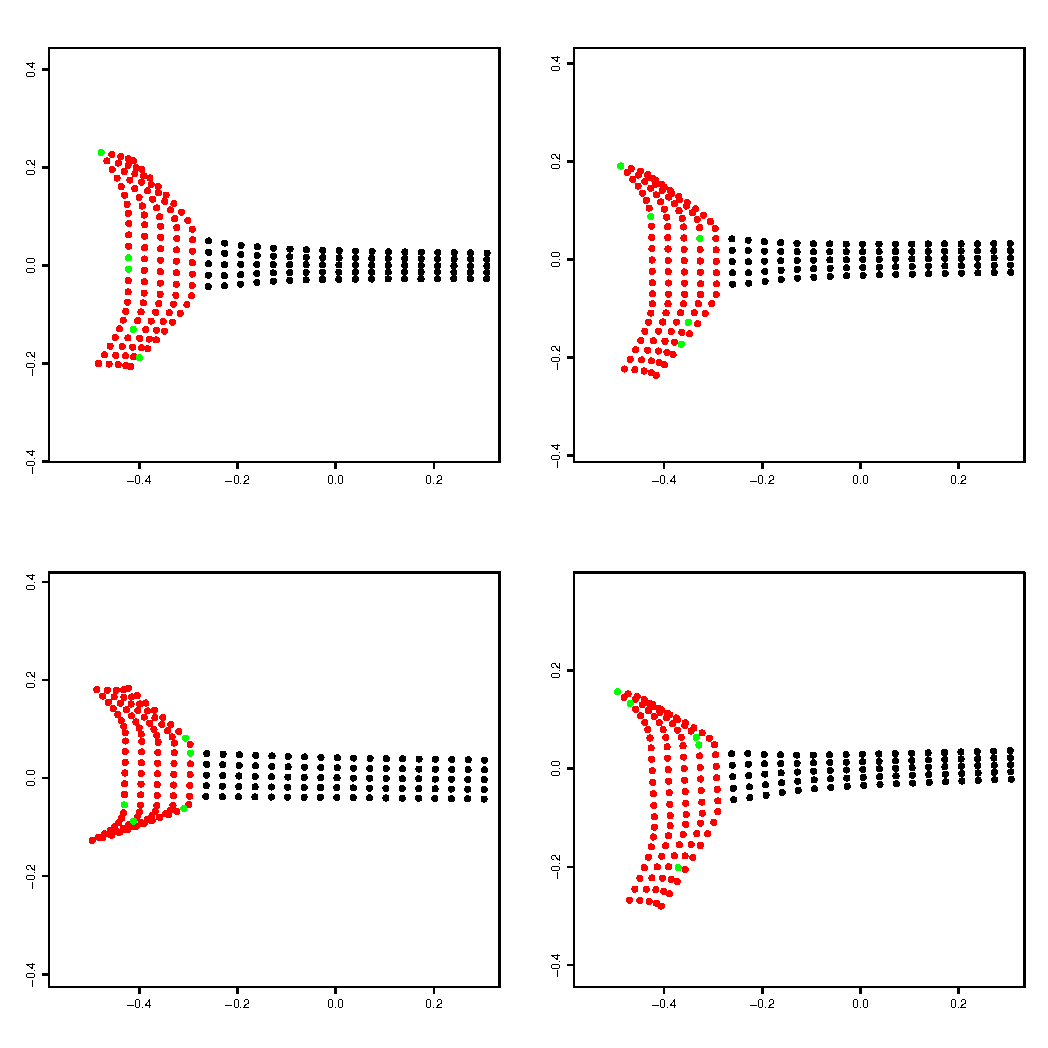
\includegraphics[width=3.5in]{mds/figs/tshaperand.pdf} \\
\caption{Using the T-shape in \fig{tshape} (top left), the tail (black points) of the T was used with 5 randomly sampled (green) points in the head. The head (without the 5 green points) was then inserted into the MDS configuration (red). As can be seen from these four realisations, the output varies greatly depending on the points sampled.}
\label{tshaperand}
% generated using figs/gridtest.R
\end{figure}

Hence, although there are the usual problems with predicting outside of the data, the added problem of the instability of MDS insertion can only confound results further. (Again, this is mentioned at the end of Gower's paper).

This problem can be rectified by using an appropriately spaced grid on the domain to calculate the eigen-decomposition, thus ensuring that the whole domain is covered. The base MDS configuration is then stable, provided that the grid is fine enough to catch all of the important features in the boundary of the domain.

\subsubsection{Smoothness of mapping}
\label{mds-smoothness}

Following from this, it is important to make sure that the MDS space is smooth in the sense that a grid of smooth lines over the domain are mapped to a series of smooth lines without discontinuities or sudden changes in direction. Taking the evenly spaced 50 by 50 point grid in \fig{wt2-grid-orig}, first MDS is performed on a dense point set of size 1253, and then a less dense grid is inserted using the method of Gower. The grid produced under the insertion can be seen in \fig{wt2-grid-full}. Taking a sample of 250 points from the 1253, an MDS configuration was also found and the same grid inserted (see \fig{wt2-grid-samp}). From this it is clear that those points mapped into the domain are smooth but in the sample case the features in the far right of the shape (the less pronounced peninsulae) are slightly squashed.

% grid to map
\begin{figure}
\centering
% trim order l b r t
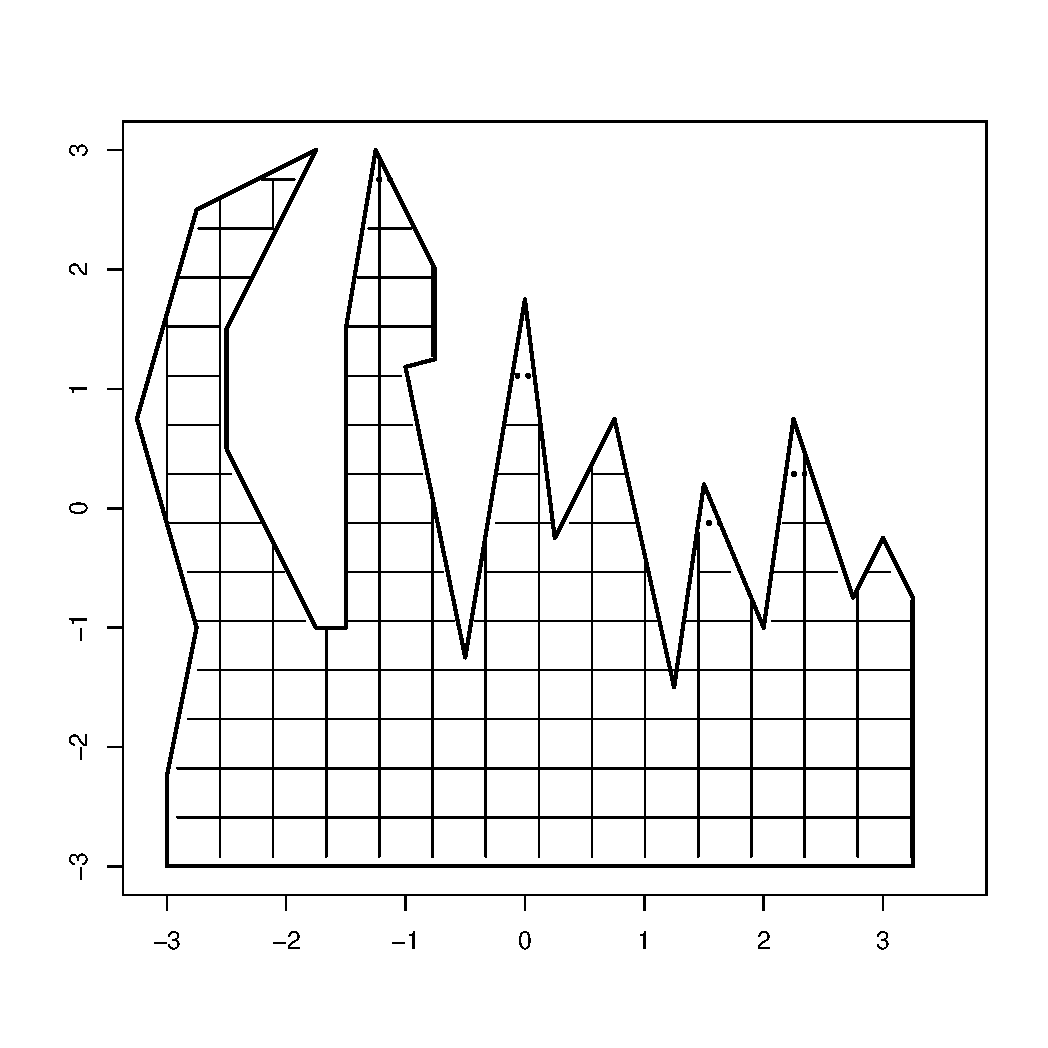
\includegraphics[width=4in]{mds/figs/wt2-grid-orig.pdf} \\
\caption{The grid to be inserted into the MDS configuration over the peninsula domain to test the smoothness of the mapping.}
\label{wt2-grid-orig}
% generated using wt2-grid.R
\end{figure}

% mapped grid (full)
\begin{figure}
\centering
% trim order l b r t
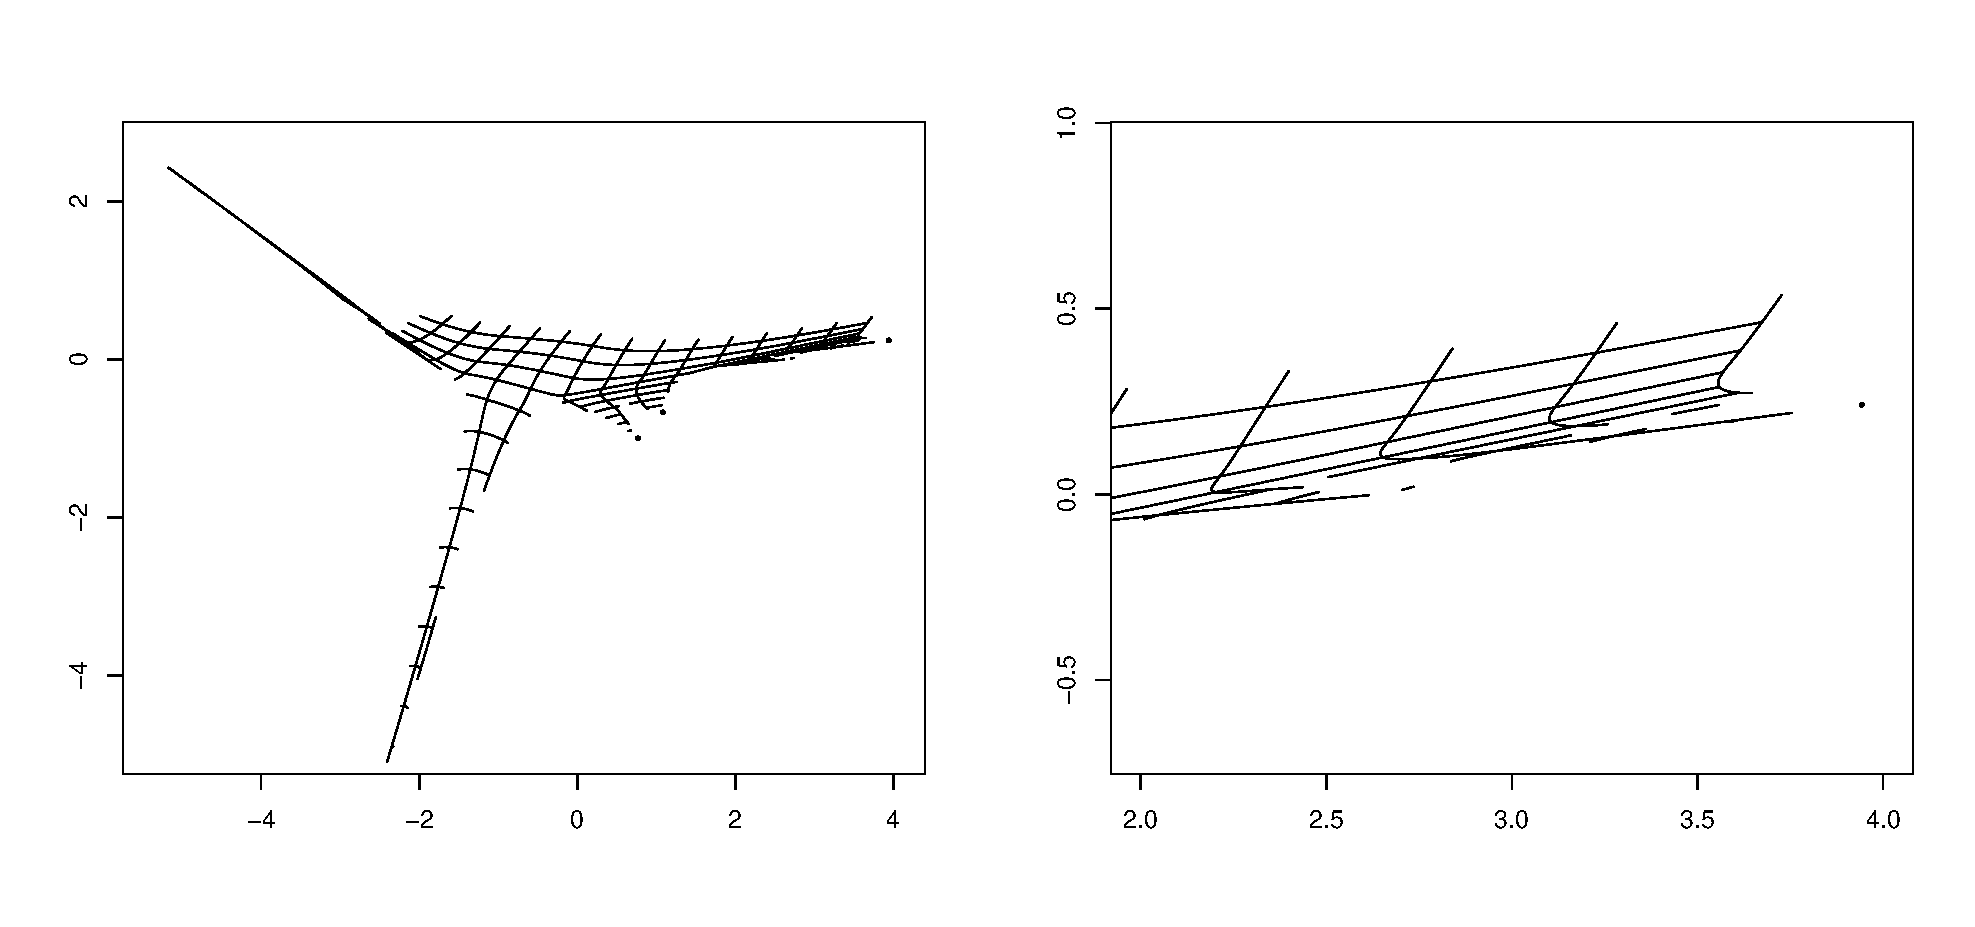
\includegraphics[width=5in]{mds/figs/wt2-grid-full.pdf} \\
\caption{Inserted grid when 1253 points are used to create the initial MDS configuration. The right panel shows a zoom of the far right part of the configuration.}
\label{wt2-grid-full}
% generated using wt2-grid.R
\end{figure}

% mapped grid (samp)
\begin{figure}
\centering
% trim order l b r t
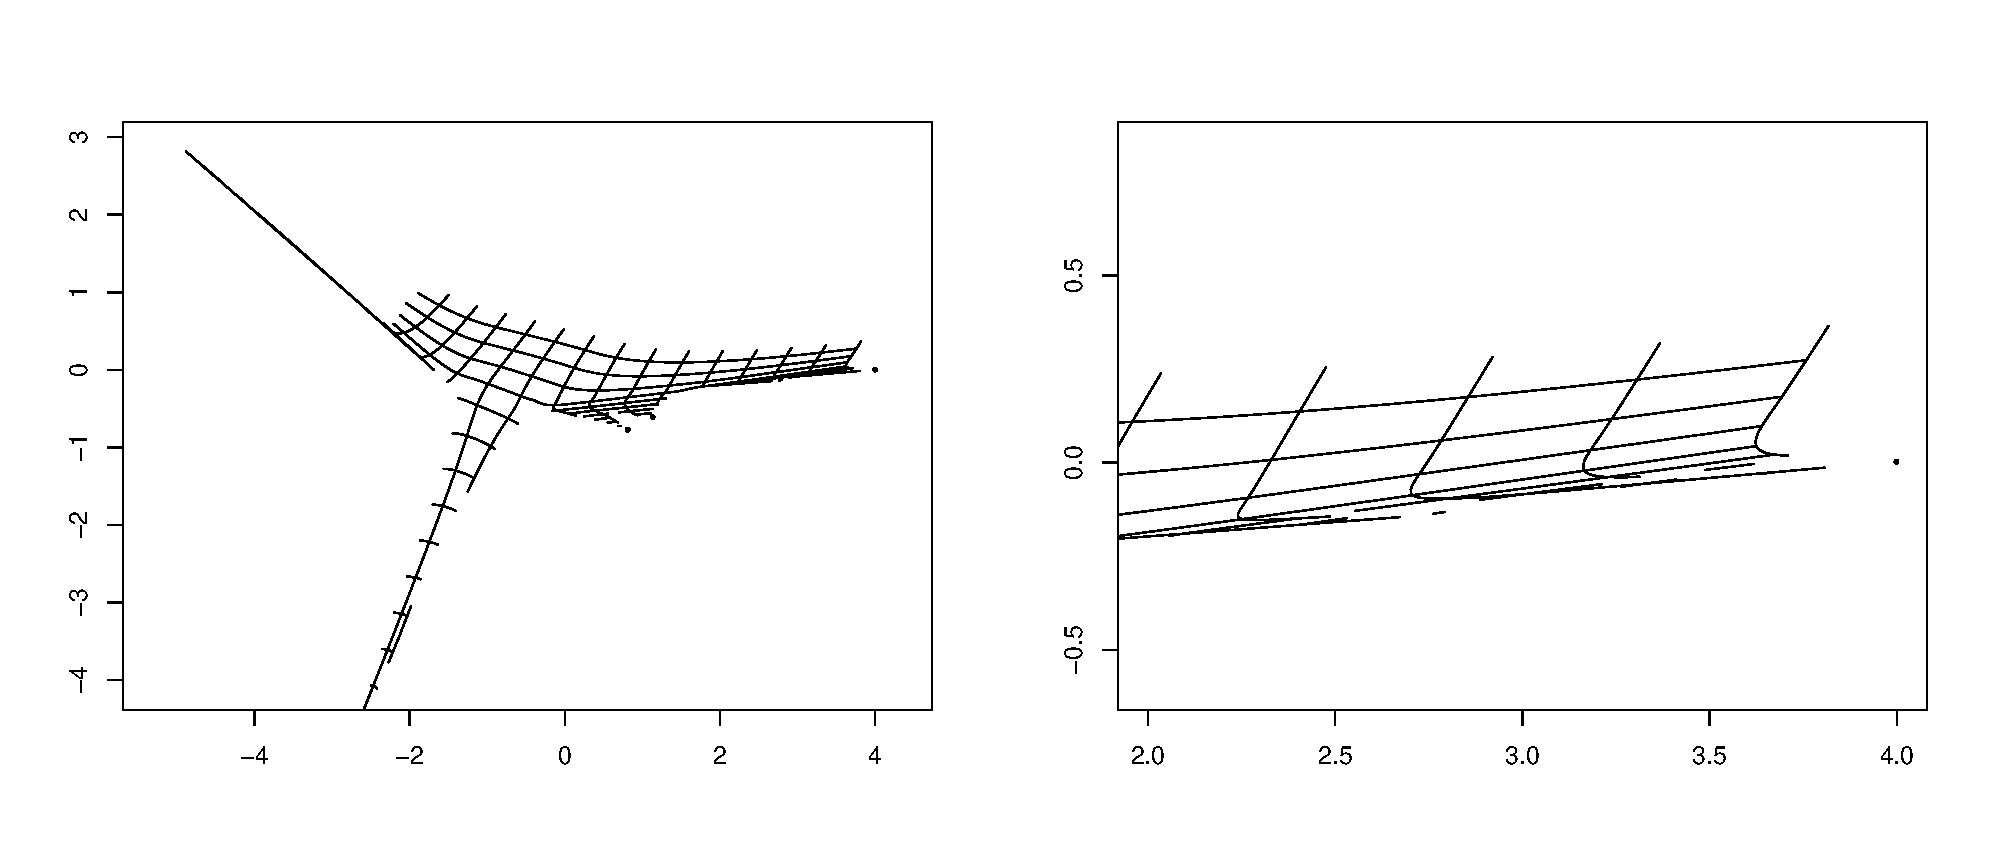
\includegraphics[width=5in]{mds/figs/wt2-grid-samp.pdf} \\
\caption{Inserted grid when 250 randomly chosen points are used to create the initial MDS configuration. The right panel shows a zoom of the far right part of the configuration. Comparing this to that of \fig{wt2-grid-full}, one can see that the features on the right have been squashed together.}
\label{wt2-grid-samp}
% generated using wt2-grid.R
\end{figure}

In conclusion, the mapping can be both reliable and also produces a smooth configuration of points provided that the initial MDS configuration covers the space in sufficient detail.


\section{Finding the within-area distances}
\label{mdsdist}
In order to perform multidimensional scaling the matrix of distances must be found. This section describes a novel algorithm to find the within-area distances.

Let the domain boundary be some polygon, $\Gamma$. Given that there is no direct path within the domain between two points ($p_1$ and $p_2$, say), the algorithm proceeds as follows to create a path (ie. an ordered set of edges and vertices), $\mathcal{P}$:

\begin{enumerate}
\item (INIT) Start by drawing a line between $p_1$ and $p_2$ (\fig{wdia}, ($i$)). Start the path as the lines from $p_1$, $p_2$ to their nearest intersection with the boundary of $\Gamma$ ($p_1^1$, $p_2^1$, say). Then form two paths. The first path from $p_1^1$ to $p_2^1$ ($\mathcal{P}_1$) contains the vertices of $\Gamma$ found moving along the boundary from $p_1^1$ to $p_2^1$. The second ($\mathcal{P}_2$), is found by taking the path from $p_1^1$ to $p_2^1$ in the other direction around the boundary, ie. the vertices of $\Gamma$ not in the first path. It is easy to see that $\{\mathcal{P}_1 \cup \mathcal{P}_2\} \setminus \{p_1^1, p_2^1\} = \Gamma$. The DELETE step (below) is then performed on $\mathcal{P}_1$ and $\mathcal{P}_2$, removing any superfluous vertices. Finding the length of $\mathcal{P}_1$ and $\mathcal{P}_2$ and choosing the shorter ($\mathcal{P^*}$), the initial path is formed as $\mathcal{P}=(p_1,p_1^1,\mathcal{P}^*,p_2^1,p_2)$. 

In \fig{wdia}, ($iii$), $\mathcal{P}_1$ is marked in green and is chosen to form the initial path, $\mathcal{P}=(p_1,p_1^1,\mathcal{P}_1,p_2^1,p_2)$, as $\mathcal{P}_1$ is shorter than $\mathcal{P}_2$, in red.

\item (DELETE) Given a triple of vertices, $(v_i, v_{i+1}, v_{i+2}) \in \mathcal{P}$ , if the line between $v_i$ and $v_{i+2}$ is shorter than the path $(v_i, v_{i+1}, v_{i+2})$ and the line between $v_i$ and $v_{i+2}$ lies inside $\Gamma$ then delete $v_{i+1}$ (\fig{wdia}, ($iv$) and ($vi$)). The entire path is iterated over deleting all superfluous vertices until there are no changes in successive runs. 

For example in \fig{wdia} ($iii$), $v_2$ is deleted from $\mathcal{P}$ because the path straight between $v_1$ and $v_3$ is shorter, and within $\Gamma$.

\item (ALTER) Given a triple of vertices $(v_i, v_{i+1}, v_{i+2}) \in \mathcal{P}$, if the path $\mathcal{P}_{ID}$ is shorter than the path $(v_i, v_{i+1}, v_{i+2})$ then replace $(v_i, v_{i+1}, v_{i+2})$ with $\mathcal{P}_{ID}$ (\fig{wdia}, ($v$)). The candidate replacement path, $\mathcal{P}_{ID}$, is calculated by running INIT with $p_1$ and $p_2$ replaced by $v_i$ and $v_{i+2}$, producing $\mathcal{P}_I$, and then using DELETE on $\mathcal{P}_I$ to remove superfluous vertices, giving $\mathcal{P}_{ID}$.

For example in \fig{wdia} ($iv$), the path $(v_1, v_2, v_3)$ is longer than the path $\mathcal{P}_{ID}=(v_1, v^1_2, v_3)$ (green dashed line in ($iv$)) so the former is replaced with the latter in $\mathcal{P}$. The path created by INIT is marked as $\mathcal{P}_{I}$ in  ($iv$) in red.

\item (ITER) We then iterate further DELETE and ALTER steps until there has been no change in $\mathcal{P}$ from one run to the next (ie. convergence) (\fig{wdia}, ($vi$)).
\end{enumerate}

% diagram for finding the shortest path in W
\begin{sidewaysfigure}
\centering
% trim order l b r t
\psfrag{exp1}[]{$\mathcal{P}_1$}
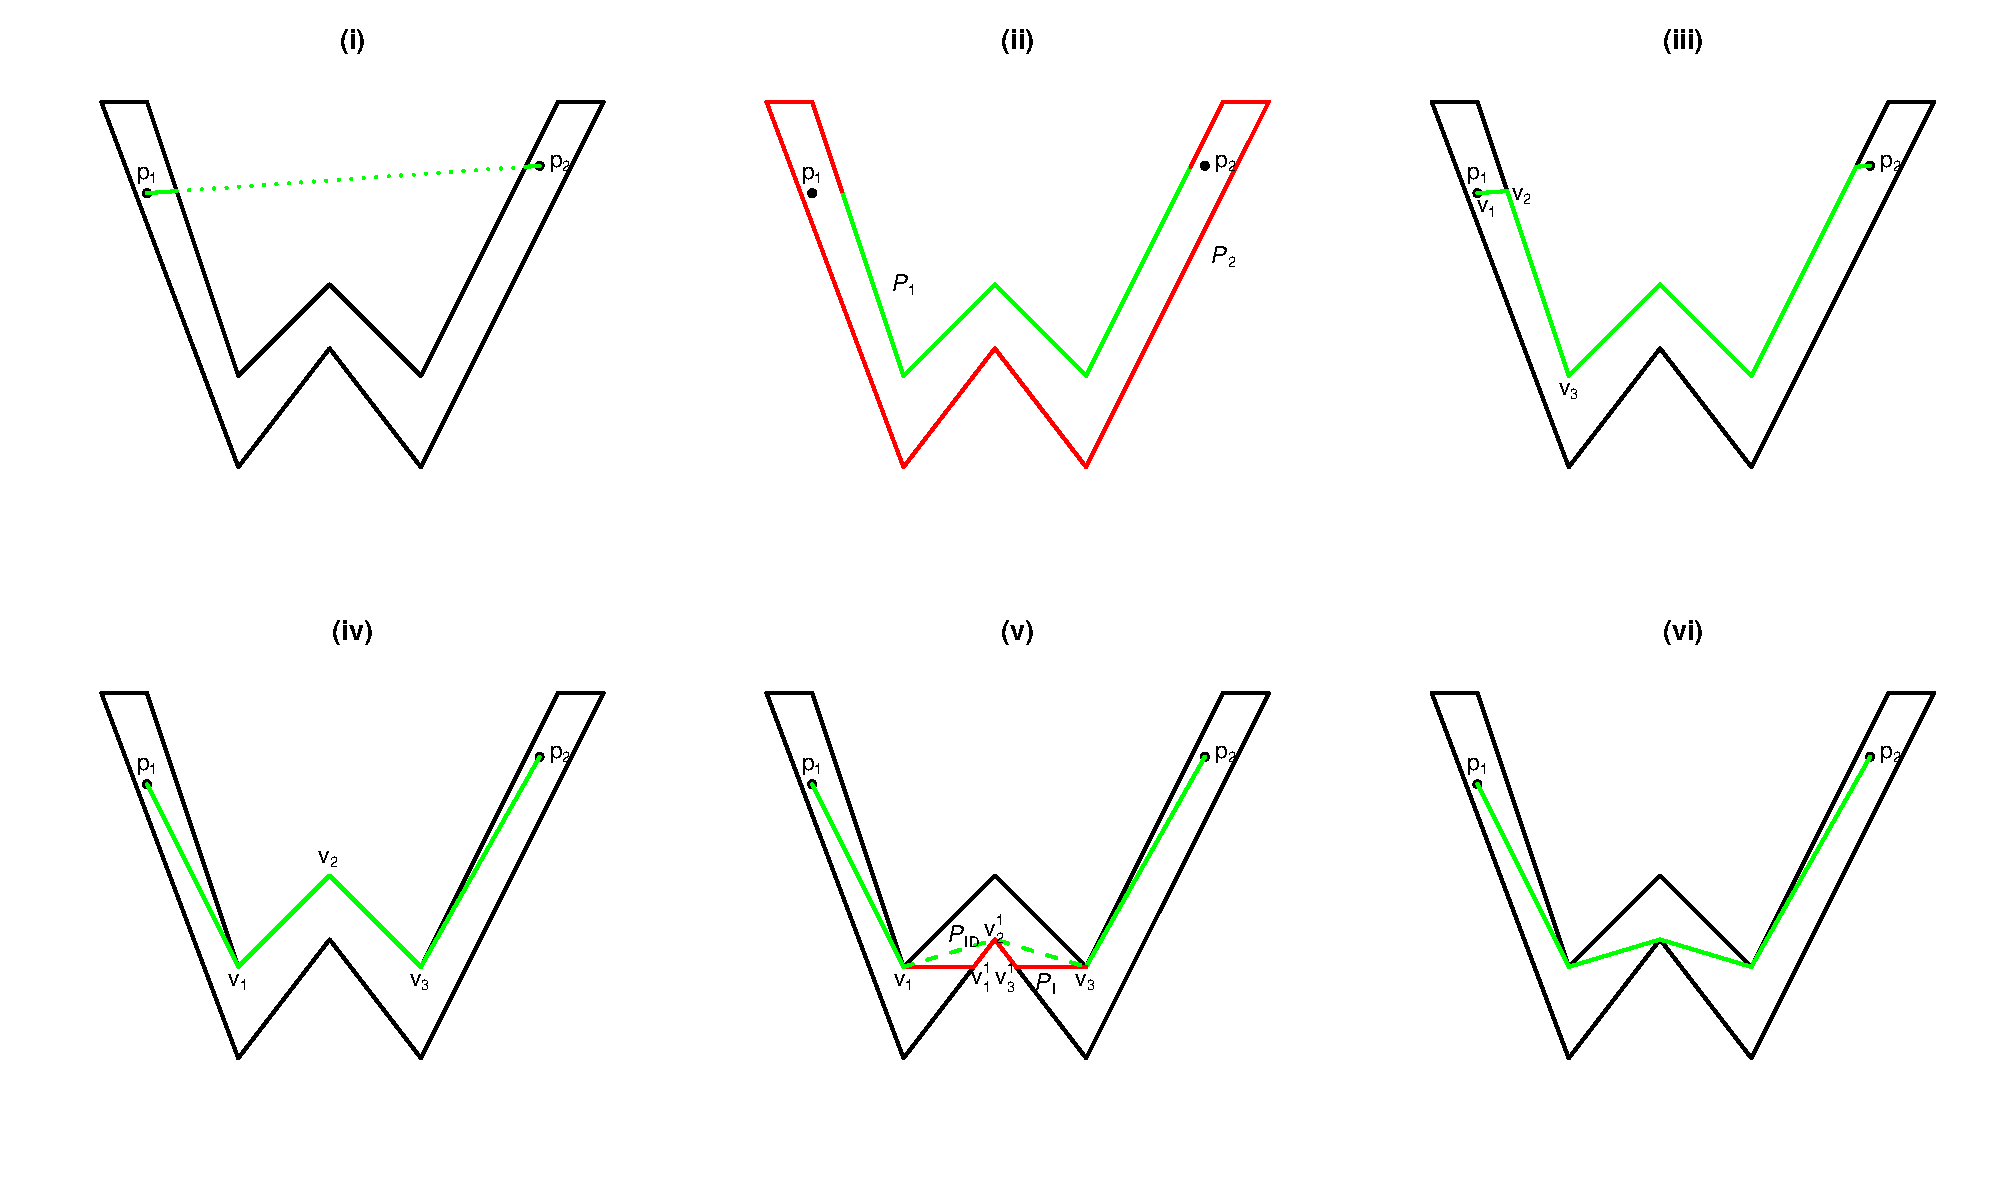
\includegraphics[trim=0in 0.5in 0in 0.25in, width=9.5in]{mds/figs/wdia.pdf} \\
\caption{The green lines in ($i$) to ($vi$) show the steps forming the shortest path as the algorithm progresses from initial state to final, shortest path (bottom right). See \secref{mdsdist}.}
\label{wdia}
% generate /phd-smoothing/mds-writeup/figs/distanceexplanation.R
\end{sidewaysfigure}

Of course, if there is a direct path between $p_1$ and $p_2$ then the Euclidean distance between the points can be used.

\section{Simulation experiments}
\label{mdssims}

In order to investigate the efficacy of \mdsap, a series of simulation experiments were performed. In all cases the results for \mdsap\ were compared to those of the current best method (the soap film smoother) and the standard approach of a {\tprs\} was used (which will not account for leakage).

The \textsf{R} packages \texttt{mgcv} and \texttt{soap} with additional bespoke software for finding the within-area distances were used. In all cases smoothing parameter estimation was performed using GCV (see \secref{GAMGCV}).

\subsection{The Ramsay horseshoe}

Again, we start with the modified Ramsay horseshoe since it clearly illustrates the problem of leakage; if a general method is to be useful it must first perform well on even a simple case such as this.

\subsubsection{Setup}

For the horseshoe, samples of 250 points with normal errors (at 3 levels:  $\sigma= $ 0.1, 1 and 10) were taken. (These are the settings used in \cite{soap}.) Using these samples, three models were fitted to the data. Predictions were then made over 718 points (including the sample locations). 200 realisations were generated and the EDF and MSE recorded for each replicate. The three models fitted were as follows:

\begin{enumerate}
\item \emph{Thin plate spline}: bivariate \tprs\  with basis size 100.
\item \emph{Soap film smoother}: 32 knots evenly spread over a grid over the domain, cyclic spline on the boundary was of basis size 39.
\item \emph{\mdsap}: Used a thin plate spline of basis dimension 100. The initial MDS grid was 20 points wide by 10 points tall.
\end{enumerate} 

Note that due to time and computational restrictions, the boundary was reduced from the 160 vertex polygon in the \texttt{fs.boundary()} function in \texttt{soap} to a 21 vertex polygon by only using every 8$^\text{th}$ vertex. This should not cause a major difference in results even if the soap film used the full boundary and \mdsap\ used only the reduced set of edges, since objective is to allow the smoother to get a broad idea of the topology of the domain, rather than the minutiae of the boundary features.

\subsubsection{Results}

Predictions from a typical realisation can be seen from \fig{mds-ramsay-fit-1}, where $\sigma=1$ with a sample size of 250. Both the soap film smoother and \mdsap\ are able to reproduce the main features of the true horseshoe function due to their ability to respect the boundary (in the case of the soap film) or the geometry of the domain (in the case of \mdsap). The \tprs\ shows leakage as expected. This is reflected in table \ref{ramsayresultstable} where we see that the soap film smoother and \mdsap\ have significantly smaller average MSE. When the noise level is high the \mdsap\ outperforms the soap film smoother in MSE terms (and is less variable).

\begin{table}[ht]
\centering
\begin{tabular}{c c c c}
 & & MSE & \\ 
$\sigma$ & \mdsap & Soap film & Thin plate\\ 
\hline
0.1  & 0.0032 (3$\cross10^{-5}$) & 0.0022 (3$\cross10^{-5}$) & 0.0402 (0.0008) \\ 
1  & 0.0436 (0.0015) & 0.0482 (0.0014) & 0.2306 (0.0024) \\ 
10  & 2.0652 (0.1215) & 3.0702 (0.2382) & 3.3713 (0.1133) \\ 
\end{tabular}
\begin{tabular}{c  c c c }
&  & EDF & \\ 
$\sigma$ & \mdsap & Soap film & Thin plate\\ 
\hline
0.1 & 47.613 (0.3497) & 39.164 (0.26) & 92.5996 (0.1020)\\ 
1  & 8.3828 (0.3452) & 11.868 (0.4010) & 46.607 (0.4238)\\ 
10 & 5.0577 (0.3324) & 5.5863 (0.2876) & 5.9786 (0.2511)\\ 
\end{tabular}
\caption{Mean MSE and estimated degrees of freedom (EDF) for the three models fitted to the modified Ramsay horseshoe function with standard errors (in brackets) over 200 realisations. Sample size was 250 with error levels given in the column marked $\sigma$.}
\label{ramsayresultstable}
\end{table}

The EDFs in table \ref{ramsayresultstable} show that \mdsap\ fits a less complex model than the thin plate spline on average, and for the two higher error situations, has a lower EDF than the soap film. Given that this is coupled with a lower MSE, it appears that \mdsap\ simultaneously yields both a more accurate and less complex model than the soap film for the horseshoe when there is a high level of noise. When noise is lower, the soap film and \mdsap\ MSEs are still of the same order. \Fig{mds-ramsay-boxplot} shows the logarithm of the per-realisation average MSE for each of the models at each error level.

% boxplot for Ramsay
\begin{figure}
\centering
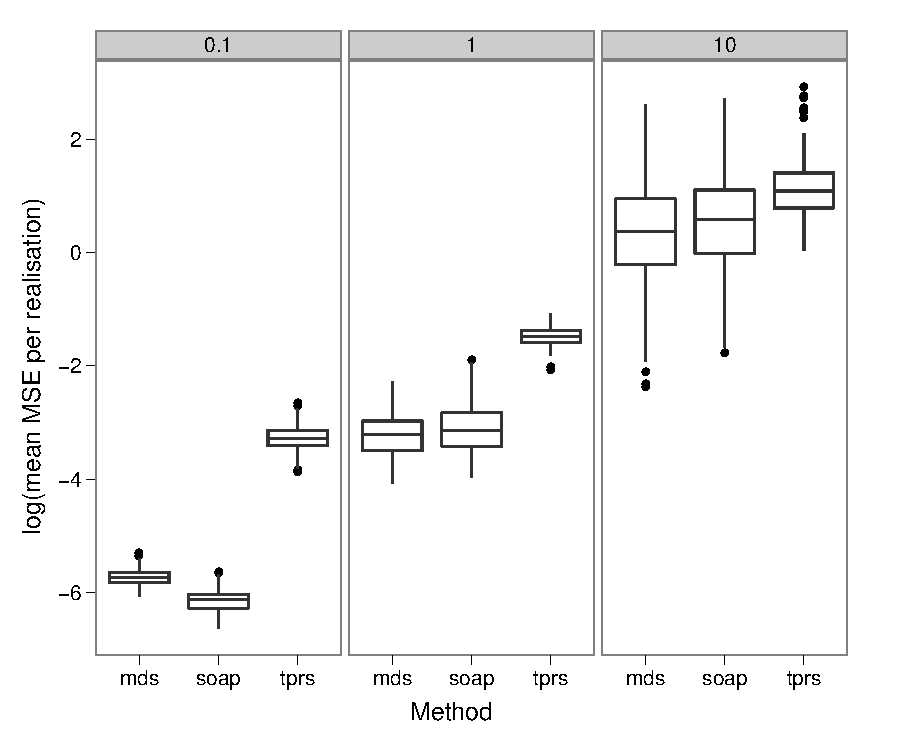
\includegraphics[width=6in, trim=0in 0.5in 0in 0in]{mds/figs/mds-ramsay-boxplot.pdf} \\
\caption{Boxplots of the logarithm of the MSE per realisation of the Ramsay horseshoe for \mdsap\, the soap film smoother and \tprs\ for error levels $\sigma=$ 0.1, 1 and 10 (left to right, respectively). In all cases, a Wilcoxon signed rank test showed that MSEs for \mdsap\ and \tprs\ were significantly different from the soap film smoother ($\text{p-value} < 10^{-2}$).}
\label{mds-ramsay-boxplot}
% generated using phd-smoothing/mds/sim/ramsay-boxplots.R
% Wilcoxon test in phd-smoothing/mds/sim/ramsay-wilcox.R
\end{figure}

% Ramsay fit with error=1 
\begin{figure}
\centering
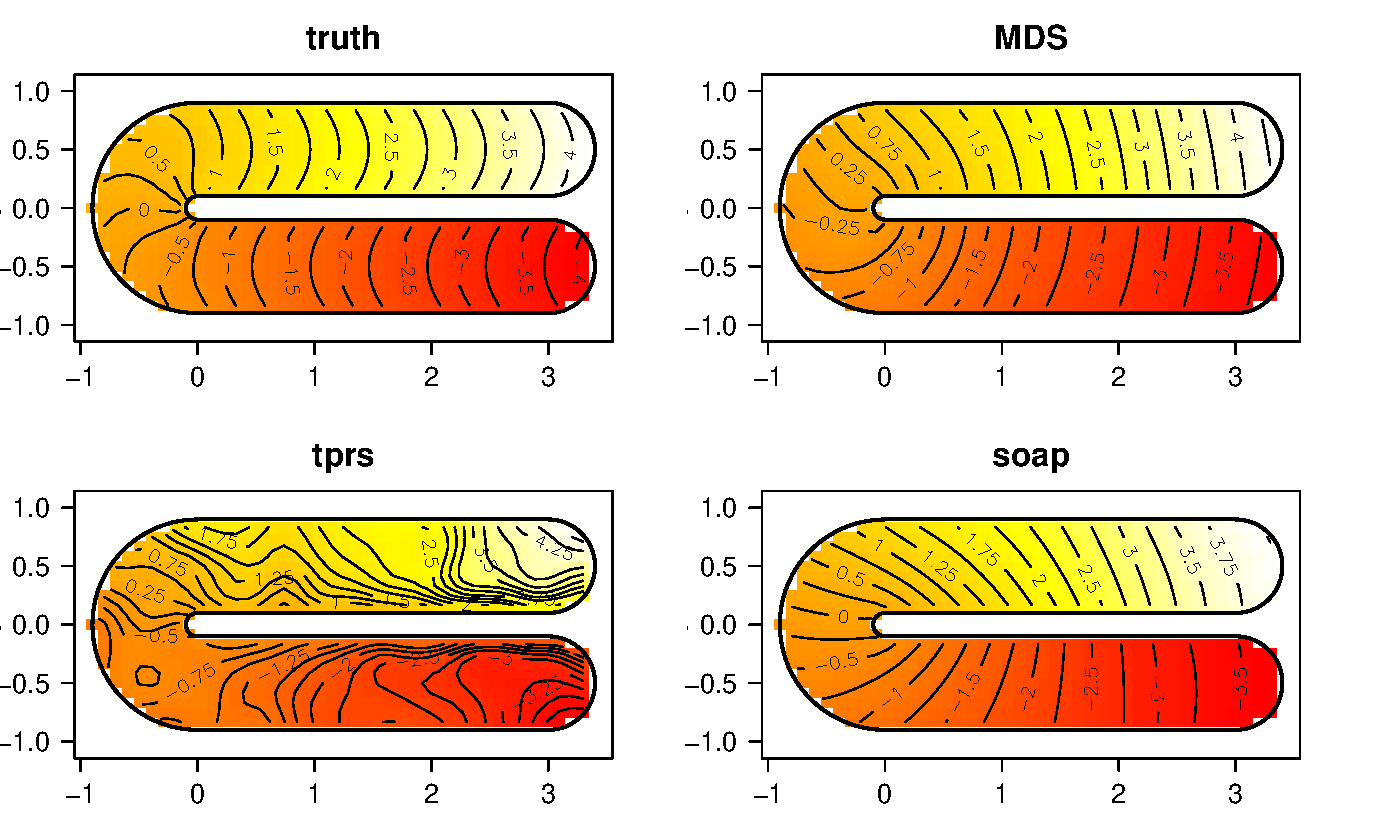
\includegraphics[width=6in]{mds/figs/ramsay-fit-1.pdf} \\
\caption{Top left: truth for the (modified) Ramsay horseshoe. Others: a typical realisation of fits from the three models when 250 points are sampled with noise set to $\sigma=1$.}
\label{mds-ramsay-fit-1}
% generated (roughly) using ramsay-smooth-test.R
\end{figure}

Just as when the \sch\ transform was used to morph the domain, it is interesting to see what has happened to the distribution of points in space. \Fig{mdsrampoints} shows the effect of the transform on a regular grid of points (left) when they are projected into MDS space (right). The projection has also succeeded in parting the two arms of the horseshoe, reducing leakage (as can be seen in the realisations in \fig{mds-ramsay-fit-1}).

\begin{figure}
\centering
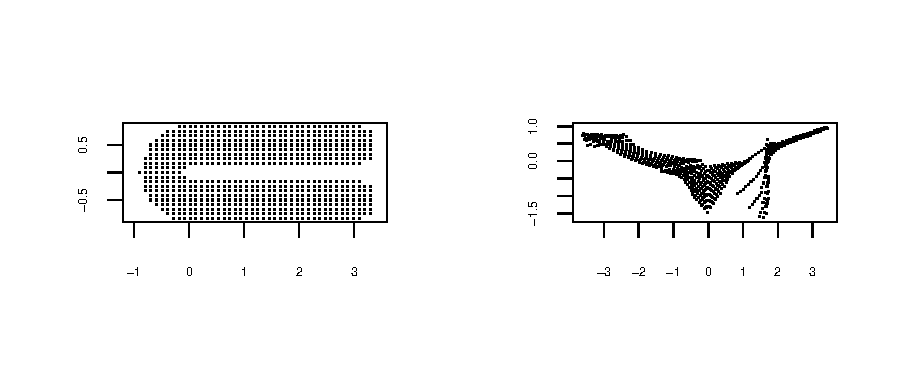
\includegraphics[width=6in,trim=0.5in 0.5in 0in 0.5in]{mds/figs/mdsrampoints.pdf} \\
\caption{A regular grid over the Ramsay horseshoe (left) and its projection into MDS space (right).}
\label{mdsrampoints}
% generated using thesis/mds/figs/mdsrampoints
\end{figure}


\subsection{Peninsula domain}
\label{mds-wt2-sim}

The Ramsay horseshoe is an easy domain to smooth over since it is clear that a transformation should be parting the two arms of the domain. In practise however, there may be ambiguity over which parts of the domain should be separated the most. For this reason a more realistic, complex domain would provide a better insight into the efficacy of the method. The domain shown in \fig{wt2-truth} is an approximation to a coastline with a strong trend along both peninsulae (in a manner similar to that of the horseshoe) but with the added complication of a further peak in the lower right corner.

\subsubsection{Setup}

The simulations consisted of 200 realisations of 250 samples from the surface in \fig{wt2-truth}. Normal errors were added at three levels $\sigma=$ 0.35, 0.9, and 1.55 (corresponding to signal-to-noise ratios (SNRs) of 0.95, 0.75 and 0.5, respectively. SNRs were calculated as the mean squared correlation between true function value and the truth with error added). Mean squared error over 1253 prediction points (including those points in the sample) was calculated and recorded, along with EDF for each model. The models fitted were:

% wt2 truth 
\begin{figure}
\centering
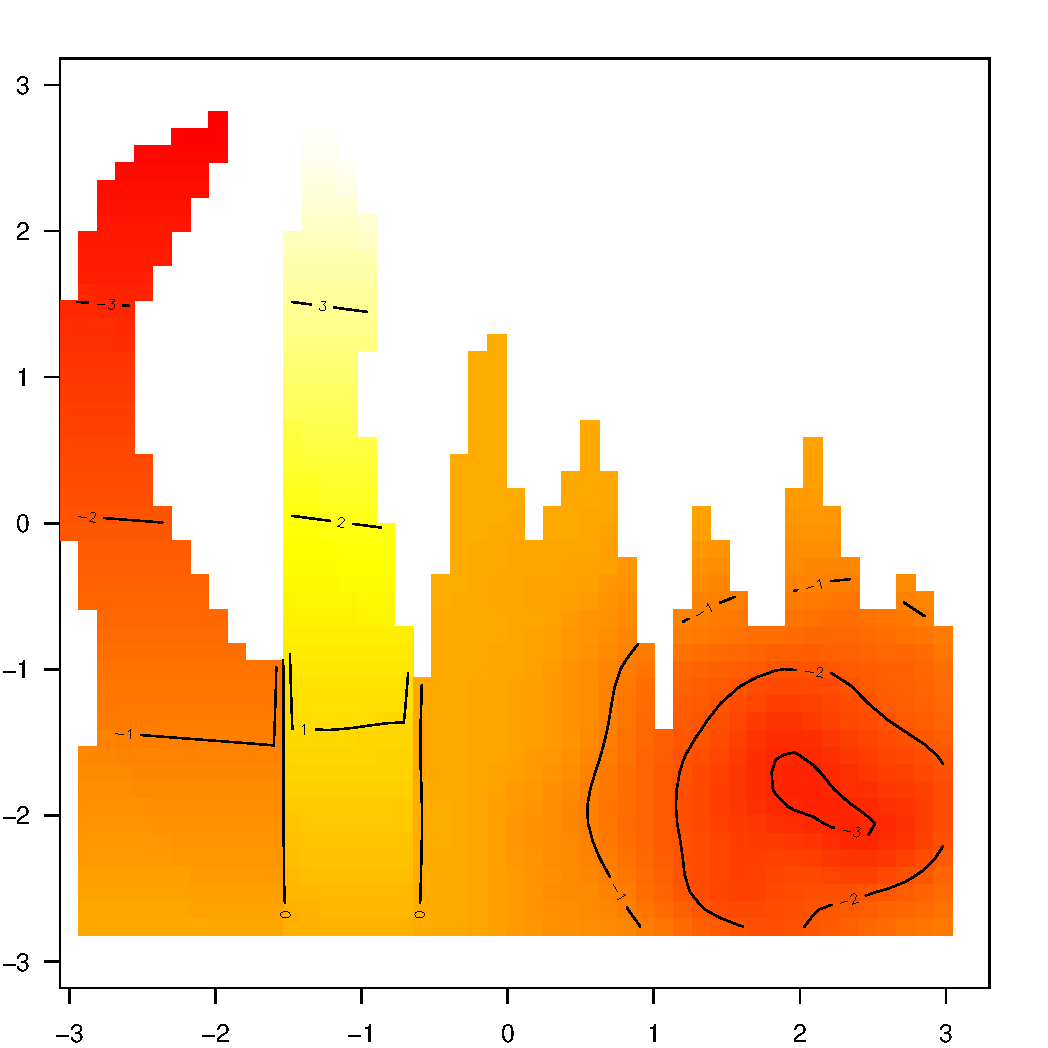
\includegraphics[width=3in]{mds/figs/wt2-truth.pdf} \\
\caption{True function for the domain with multiple peninsulae.}
\label{wt2-truth}
% generated (roughly) using wt2-smooth-test.R
\end{figure}

\begin{enumerate}
\item \emph{Thin plate spline}: bivariate thin plate spline with basis size 100. 
\item \emph{Soap film smoother}: cyclic spline on boundary of basis size 60, 109 internal knots evenly spaced on a grid over the domain.
\item \emph{\mdsap}: after transform a bivariate thin plate spline with basis size 100 was fit. The initial MDS grid was 10 by 10 points square (48 points were inside).
%\item \emph{MDS with tensor product}: tensor product of two thin plate splines, each of basis dimension 12. The initial MDS grid was 74 points square.
\end{enumerate} 

\subsubsection{Results}

% wt2 fit with error=0.9
\begin{figure}
\centering
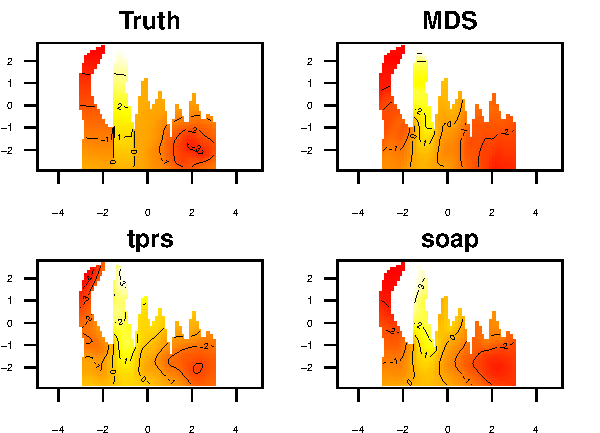
\includegraphics[width=6in]{mds/figs/wt2-comp-09.pdf} \\
\caption{A typical realisation of fits from the multiple peninsulae domain when $\sigma$ is set to 0.9 (SNR = 0.75) and sample size is 250. Prediction grid was of size 1253. Clockwise from top left: the true function, prediction from: MDS projection smoothed with \tprs, the soap film smoother and \tprs.}
\label{wt2-comp-0.9}
% generated (roughly) using wt2-smooth-test.R
\end{figure}

Looking at a typical realisation in \fig{wt2-comp-0.9} ($\sigma=$ 0.9, SNR = 0.75, sample size 250), the \tprs\ can be seen showing signs on leakage across the two main peninsulae, whereas \mdsap\ and the soap film do not show this. However the \tprs\ does reproduce the peak in the lower right much more faithfully, the other two smoothing over it. In this realisation, \mdsap\ deals with the values inside the peninsula a little better than the soap film smoother (the contour lines are closer to those in the true function). On the other hand, the soap film captures the shape of the lower right peak slightly more accurately.

Table \ref{wt2resultstable} gives the MSE and EDF for the models above averaged over 200 realisations. There is not a massive difference between the results in MSE terms, the soap film smoother consistently has a lower MSE, although not by much. The soap film also tends to fit simpler models than the other two approaches. The boxplots of the logarithm of the per-realisation MSEs are shown in \fig{mds-wt2-boxplot}.

% boxplot for wt2
\begin{figure}
\centering
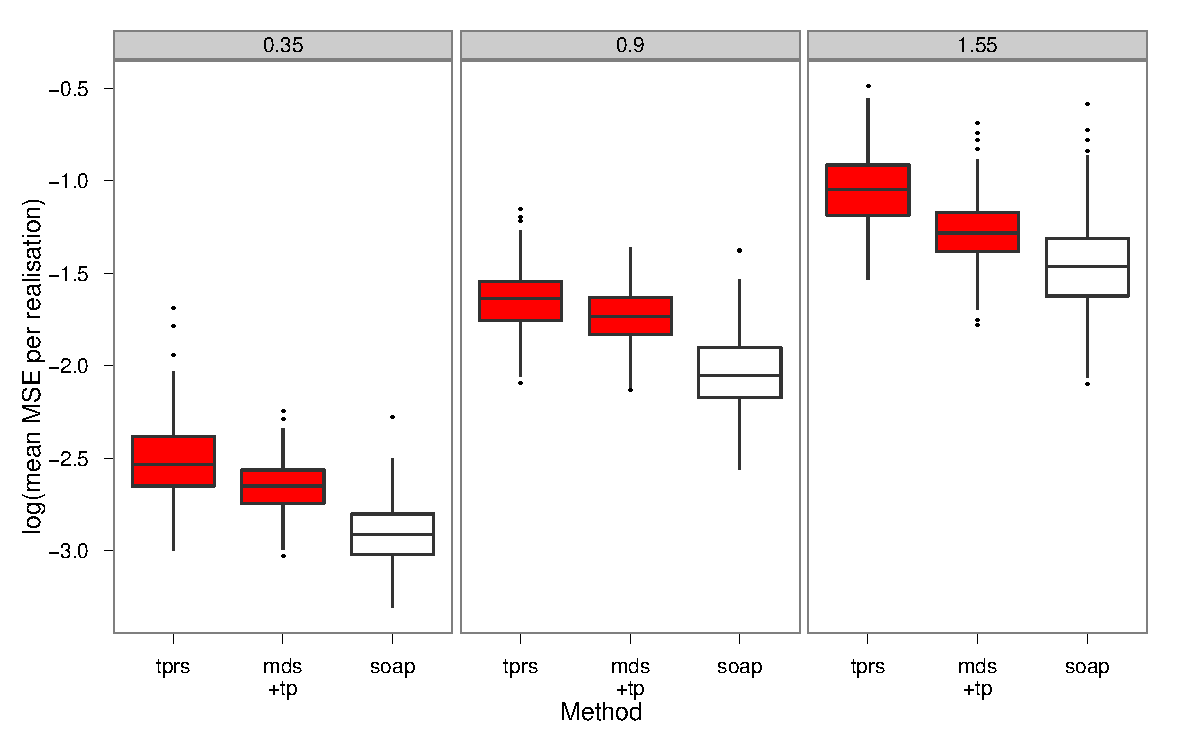
\includegraphics[width=6in, trim=0in 0.5in 0in 0in]{mds/figs/mds-wt2-boxplot.pdf} \\
\caption{Boxplots of the logarithm of the MSE per realisation of the peninsula domain for the MDS approach, soap film smoother and \tprs\ for error levels $\sigma=$ 0.35, 0.9 and 1.55 (left to right, respectively). A Wilcoxon signed rank test shows that the MSEs for \tprs\ were significantly different from those of the soap film smoother ($\text{p-value} < 10^{-2}$) at all noise levels. For \mdsap\ the two lower noise cases were significantly different from the soap film smoother, but not when $\sigma=1.55$ ($\text{p-value} = 0.023951$).}
\label{mds-wt2-boxplot}
% generated using phd-smoothing/mds/sim/wt2-boxplots.R
\end{figure}

\begin{table}[ht]
\centering
\begin{tabular}{c c c c c}
 &  & MSE  & &\\ 
$\sigma$ & \mdsap & Soap film & Thin plate\\ 
\hline
0.35  & 0.07 (0.00062) & 0.0539 (5e-04) &0.082 (0.00104)\\
0.9  & 0.177 (0.00184) & 0.1308 (0.00197) &0.1938 (0.00241)\\
1.55  & 0.2859 (0.00438) & 0.2362 (0.00434) &0.3509 (0.00471)\\
\end{tabular}
\begin{tabular}{c c c c c}
 &  & EDF  & &\\ 
$\sigma$ & \mdsap & Soap film & Thin plate\\ 
\hline
0.35 &80.9039 (0.57103) & 55.6979 (0.51448) & 77.9619 (0.46726)\\ 
0.9 &35.0185 (0.76449) & 29.7171 (0.57477) & 48.0508 (0.47636)\\ 
1.55 &19.4625 (0.57265) & 20.2918 (0.36634) & 32.2715 (0.47961)\\ 
\end{tabular}
\caption{Mean MSE and EDF for the four models fitted to the peninsula domain with standard errors (in brackets) over 200 realisations.}
\label{wt2resultstable}
\end{table}

As with the Ramsay horseshoe, it is interesting to see what the projection into MDS space has done to the distribution of the points in the domain. \Fig{wt2-2d-proj} shows points in the domain in Euclidean space and MDS space. There appears to be some high concentrations of points in the far left peninsula and in the right side in the MDS space. This is due to the projection from $n$-dimensional space into 2-dimensional space, which can be easily seen in \fig{wt2-3d-proj} where the points have been projected into 3-dimensional space. This shows that there is separation between the smaller peninsulae in higher dimensions that cannot be seen in the 2-dimensional projection.

This high point density in the right side of the MDS space could be the reason for the poor reproduction of the function in that region, seen in \fig{wt2-comp-0.9}. In this portion of space (and in the left peninsula) there is a breakdown in isotropy, which the \tprs\ does not handle well. This must be accounted for in the smooth if accurate models are to be built.

% how the points are projected for wt2
\begin{figure}
\centering
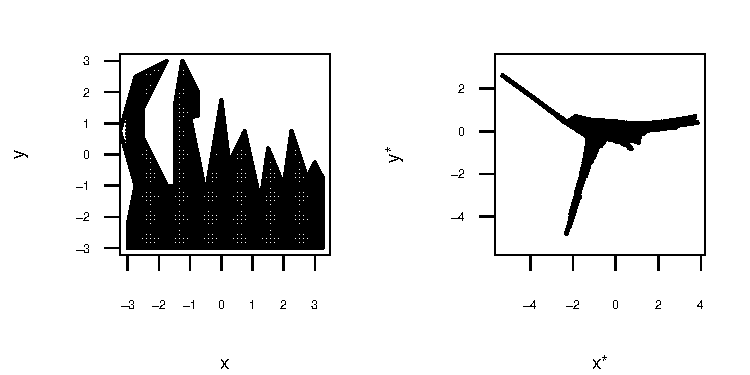
\includegraphics[width=6in]{mds/figs/wt2-2d-proj.pdf} \\
\caption{A regular grid over the peninulae domain (left) and its projection into MDS space (right).}
\label{wt2-2d-proj}
% generated using thesis/mds/figs/wt2-mds.R
\end{figure}

% how the points are projected for wt2 in 3D!
\begin{sidewaysfigure}
\centering
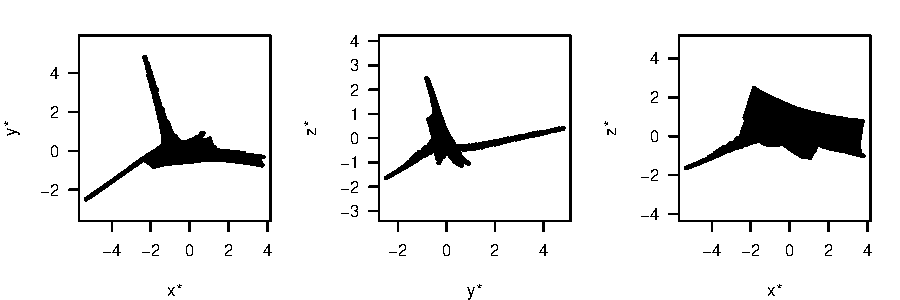
\includegraphics[width=9in]{mds/figs/wt2-3d-proj.pdf} \\
\caption{The peninsula domain projected into 3-dimensional MDS space. The plots show combinations of axes, note that the $x^*,y^*$ combination is the same as the 2-dimensional projection in \fig{wt2-2d-proj}.}
\label{wt2-3d-proj}
% generated using thesis/mds/figs/wt2-mds.R
\end{sidewaysfigure}

\subsection{Areas for improvement}

From this set of simulations areas for improvement to \mdsap\ can be seen. First, the above problem of the accuracy of the model (in terms of faithfully reproducing the function) needs to be addressed. Second, running the model is actually quite slow, the calculation of the within-area distances by the algorithm given in \secref{mdsdist} has considerable computational cost, even in comparison to the soap film smoother basis setup. Table \ref{wt2time} shows the average timings for running \mdsap, \tprs\ and soap film smoothers over the peninsula domain

\begin{table}[ht]
\centering
\begin{tabular}{c || c c c c c c}
 & \mdsap & Soap film & Thin plate\\ 
\hline
Fit & 84.85242 & 24.6783 & 0.4022\\ 
Prediction &  53.5105 & 29.3946 & 0.1249\\
\end{tabular}
\label{wt2time}
\caption{Average time (in seconds) to fit and predict on a realisation of the peninsula domain for the four models considered above. Times are averaged over 100 realisations and were found using the elapsed time provided by \textsf{R}'s built-in \texttt{system.time} function. For each realisation a sample of size 250 was taken, then a 1253 values were predicted.}
\end{table}

In order to make \mdsap\ worthwhile for a practitioner to use the method, it would be preferable for it not only to have a sensible physical model, but also outperform the soap film smoother in either (or both) of accuracy and speed.

\section{Improvements}
\label{MDSimprov}

This section focuses on strategies to improve the above method in terms of speed and accuracy. The first part looks at the speed of \mdsap, the latter on the accuracy. 

\subsection{Making \mdsap\ faster}
\label{mds-faster}

\subsubsection{Calculating MDS by Lanczos iteration}

The \textsf{R} command used to perform the multidimensional scaling, \texttt{cmdscale}, uses the routine \texttt{eigen} in order to perform the requisite matrix eigen-decomposition. This routine will calculate a full eigen-decomposition of the matrix, even if only the first $k$ eigenvalues and/or eigenvectors are required. Using Lanczos iteration, only the first $k$ eigenvalues (in numeric or algebraic size order) will be calculated.

The  Lanczos procedure works by iteratively building a symmetric $i\cross i$ tridiagonal matrix (at the $i^{\text{th}}$ iteration) which has eigenvalues approximately the same as the $i$ largest eigenvalues of the original matrix. Further detail is given in \cite{simonbook}, pp. 335-337.

The \texttt{igraph} library for \textsf{R} provides an interface to the C++ package \texttt{ARPACK++} which implements the Lanczos procedure. Replacing the \texttt{cmdscale} command with one that uses the \texttt{ARPACK++} interface provided by \texttt{igraph} will decrease the number of computations needed, thus making the calculation of the eigenvalues and vectors faster.

A quick benchmark shows that \texttt{ARPACK++} can compute the first two eigenvalues and vectors faster than just using \texttt{eigen} when the eigen-decomposition to be computed is of a large matrix. Generating a 1000 by 1000 symmetric matrix of Normal random variates with mean 0 and variance 1000, then performing an eigen-decomposition takes 1.68 seconds using \texttt{ARPACK++} and 3.26 seconds using \texttt{eigen} (averaged over 100 runs). This advantage drops once the matrix is around 100 by 100 and the cost of calling the C++ code begins to dominate; in this case \texttt{ARPACK++} takes 0.037 seconds and \texttt{eigen} takes 0.034 (over 100 runs). Given that the disadvantage is in the order of hundredths of a second and the advantage is a two-fold decrease in computational time, it makes sense to use the \texttt{ARPACK++} code in all cases.

% sim code is at ~/phd-smoothing/mds/lanczos/time-arpack.R

\subsubsection{Partial path calculation}

Many of the distances stored in $D$ are calculated by simply using the Euclidean metric since for the corresponding point pairs, there is no part of the path between them that lies outside of the domain. It is often the case that the paths that need to be calculated are on a grid (for example, when doing prediction). This leads us to believe that there are many sets of paths that are rather similar. These paths may perhaps only differ in their final vertex. Given that, in this case, there is a lot of wasted computational time spent calculating similar paths, it would be useful to exploit this problem, and use it to increase the speed of the path calculation.

The idea here is to use a sparse grid to first calculate a set of paths that are then saved. These saved paths are then form the base of the other paths that need to be calculated. Finally, these paths are optimised in the same manner as the algorithm given in \secref{mdsdist}. This removes the expensive calculation in the middle of the path, where perhaps the bulk of the interactions with the boundary take place.

The algorithm is as follows, with notation and routines (INIT, DELETE, ALTER and ITER) identical to those in \secref{mdsdist}. 

Again, taking points $p_i$ and $p_j$ in the set of points in the domain that we wish to find the shortest paths for and drawing a path between them, finding within-area distance with respect to the boundary of $\Gamma$.

\begin{enumerate}
 \item Begin by creating a sparse grid of within $\Gamma$ and calculate the ($M$, say) non-Euclidean within-area paths between all pairs of points exactly as in \secref{mdsdist}. Store these paths as $\mathcal{P}_1,\ldots, \mathcal{P}_M$.
\item For each unique pairing of $p_i$ and $p_j$ in the full data set, calculate the path using one of the following:
	\begin{enumerate}
	\item Find a $\mathcal{P}_k$ such that the path between $p_i$ and one end of $\mathcal{P}_k$ and $p_j$ and the other end of $\mathcal{P}_k$ is Euclidean within $\Gamma$. Join $p_i$ and $p_j$ onto the appropriate ends of $\mathcal{P}_k$ and run ITER (ie. alternate between DELETE and ALTER) until convergence.
	\item If there is no Euclidean path between $p_i$ and $p_j$, and no $\mathcal{P}_k$ can be found, then calculate the path between $p_i$ and $p_j$ as in \secref{mdsdist}. 
	\end{enumerate}
\end{enumerate}

Note that those paths between points in the sparse grid which are Euclidean are not stored since it is always at least as expensive to store, add and optimise those paths then calculating them from scratch. An argument towards why is this is true is as follows: if the path we want to calculate is Euclidean anyway, then retrieving a Euclidean path, adding in $p_i$ and $p_j$, and then iterating over ALTER and DELETE steps to make it both the shortest and a Euclidean path will take longer than just creating a Euclidean path to begin with. If the path between $p_i$ and $p_j$ is non-Euclidean then the non-Euclidean part of the path must lie outside $\mathcal{P}_k$ (by definition) and therefore will take the same number of operations to find the boundary crossing points and calculate the shortest path around the feature locally as it will to calculating the whole path from scratch.


\subsubsection{Simulation - Lanczos and partial path calculation improvements}

Taking both the Lanczos procedure and the partial path calculation together, a simulation was run to find the improvements in terms of computational time for the double peninsulae domain. Average time for both model fitting and prediction are given in \tabref{wt2itime} for 100 realisations. 

The differences between the first two columns are striking. The partial path calculation has dramatically reduced the computational time for the calculation of the entries of the distance matrix, making it faster than the soap film smoother for the model fitting, and reducing the prediction time to a third of its previous value. The \tprs\ times are shown to give a comparison for the time actually taken to fit the model, the remaining time for \mdsap\ is taken up by calculating the distances and performing the MDS.

\begin{table}[ht]
\centering
\begin{tabular}{c || c c c c c c}
%  no speedup           speedup
 & \mdsap & \mdsap (\textit{pp}) & Soap film & Thin plate\\ 
\hline
Fit & 84.85242 & 18.6526 & 24.6783 & 0.4022\\ 
Prediction & 155.4004 & 53.5105 & 29.3946 & 0.1249\\
\end{tabular}
\label{wt2itime}
\caption{Average time (in seconds) to fit and predict on a realisation of the peninsula domain for the four models considered above. Times are averaged over 100 realisations and were found using the elapsed time provided by \textsf{R}'s built-in \texttt{system.time} function. For each realisation a sample of size 250 was taken, then a 1253 values were predicted. For the \mdsap\ columns \textit{pp} indicates the cases where the partial paths were pre-calculated, those not marked use the algorithm given in \secref{mdsdist}.}
\end{table}


\subsection{Improving the accuracy of \mdsap\ by adjusting the penalty}
\label{mds-penadjust}

The higher MSEs shown in \tabref{wt2resultstable} at lower noise levels might be explained by the change in density of points in the domain after it has been transformed into MDS space and the way in this changes the measure of smoothness. In this case it makes sense to adjust the penalty in order to take into account the change in point density in MDS space.

\cite{wood2000} shows that given some transform of a variable, $y$ say, such that $y_i^\prime=y_i/k$, then $f(x,y^\prime k)$ will give the same fit as $f(x,y)$ (ie. the fit will be the same under the new coordinates). In this case the penalty will change to:
\begin{equation}
\int\int_\Omega \Big( \frac{\partial^2 f}{\partial x^2} \Big)^2 + 2k\Big( \frac{\partial^2 f}{\partial x \partial y} \Big)^2 + k^3\Big( \frac{\partial^2 f}{\partial y^2} \Big)^2 \text{d}x \text{d}y,
\label{adjustedintegral}
\end{equation}
from the usual \tprs\ penalty (see \secref{GAMtprspenalty}).

This approach will only handle a linear rescaling in one dimension; in the case of the MDS distortions, non-linear re-scalings in two dimensions must be addressed. To generalise \eqn{adjustedintegral} to the non-linear two-dimensional case a function must be found, $\mathcal{L}^*(x,y)$ say, which evaluates to the change in density for each point in the domain. 

Such a function should allow the smoothness to be adapted according to the degree to which space has been squashed, thus getting around the spatial heterogeneity which appears to be affecting the model. The calculation of $\mathcal{L}^*(x,y)$ is elaborated on below.

Given that the function $\mathcal{L}^*(x,y)$ is known, the penalty is given as:
\begin{equation}
\int\int_\Omega \mathcal{L}^*(x,y) \Big( \Big(\frac{\partial^2 f(x,y)}{\partial x^2}\Big)^2 + 2\Big(\frac{\partial^2 f(x,y)}{\partial x \partial y}\Big)^2 + \Big(\frac{\partial^2 f(x,y)}{\partial y^2}\Big)^2\Big) \text{d}x\text{d}y.
\label{kdeadjust}
\end{equation}
Note the change of integration domain from $\mathbb{R}^2$ to $\Omega$ (the transformed domain), as well as the pre-multiplication by the density function.

\subsection{Penalty adjustments in one dimension}

Before implementing this approach in full a a test was run in one dimension. The function:
\be
g(x)=0.2x^{11}(10(1-x))^6+10(10x)^3(1-x)^{10},
\label{hardfcn}
\ee
was used and contracted by factors of $20,1,0.05,1$ over the regions $[0,0.4], (0.4,0.6],(0.6,0.8],(0.8,1]$, respectively. The function and its squashed form are shown in the top left and right panels (respectively) of \fig{1dadjust}. Evaluating 100, equally spaced, points over the interval $[0,1]$ using a \tprs\ and then predicting back onto the same points yielded the blue lines in the lower two plots. The left of these shows the prediction in the transformed space and the right in the original space. The green line was produced using a \tprs\ with the adjusted penalty matrix. As can be seen from the plot, the fit has been improved greatly. We now look at the calculation of the adjustment to the penalty.

% 1d adjustment 2x2 diagram
\begin{figure}
\centering
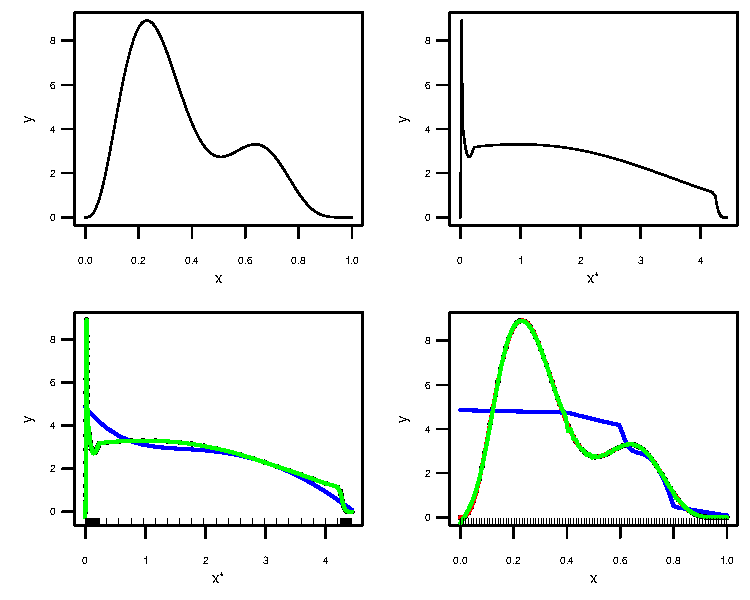
\includegraphics[width=6in]{mds/figs/1dadjust.pdf} \\
\caption{Using penalty adjustments to fit a regression spline to \eqn{hardfcn} after it has been squashed. The function in the top left is squashed to the form in the top right. The bottom left plot shows the fit from a \tprs\ (blue) and a \tprs\ with adjusted penalty (green) in the transformed space. The bottom right shows the same fit in the untransformed space. Clearly, the penalty adjustment improves the fit.}
\label{1dadjust}
% generated by thesis/mds/figs/tpintexp.R
\end{figure}

\subsubsection{Penalty adjustment calculation}

For the moment let us take $\hat{f}$ to be a one dimensional smooth function. It may be decomposed into its basis functions and coefficients in the usual way:
\be
\hat{f}(x)=\sum_{j=1}^J \hat{\beta}_j b_j(x) = \tr{\hat{\bm\beta}}\bm{b}(x).
\ee
The $ij^\text{th}$ element of the penalty matrix (see \secref{GAMpenalties}) is given as:
\be
S_{ij}= \int_a^b \mathcal{L}^*(x) \frac{\partial^2 b_i(x)}{\partial x^2}\frac{\partial^2 b_j(x)}{\partial x^2} \text{d}x = \int_a^b \mathcal{L}^*(x) b^{\prime\prime}_i(x) b^{\prime\prime}_j(x) \text{d}x,
\ee
in one dimension (letting a prime indicate differentiation with respect to $x$). The integral can then be approximated by the midpoint rule as:
\be
S_{ij}= \frac{b-a}{K}\sum_{k=1}^K \mathcal{L}^*(x_k) b^{\prime\prime}_i(x_k) b^{\prime\prime}_j(x_k) \quad \text{for} \quad x_k=a+\frac{(k-0.5)(b-a)}{K},
\label{midpointS}
\ee
for $k=1,\dots, K$. Second derivatives are evaluated by finite differences in the usual manner:
\be
\label{bfinitediff}
b^{\prime\prime}_i(x) = \frac{ b_i(x+2\epsilon) - 2b_i(x+\epsilon) + b_i(x)}{\epsilon^2}.
\ee
For the sake of efficiency, we in fact calculate a $K\cross J$ matrix $D$ with $kj^\text{th}$ element:
\be
D_{kj}=\sqrt{\mathcal{L}^*(x_k)} b^{\prime\prime}_j(x_k),
\label{oneDD}
\ee
for $x_k$ as above. Then $S$ may be calculated as:
\be
S=\frac{b-a}{K}\tr{D}D.
\ee

In this example $\mathcal{L}^*(x)$ was simply calculated using the inverse of the cube of the factor by which the relevant part of the domain (given above) was squashed. 

\subsubsection{Checking that the adjustment works}

\Fig{1dadjust} shows that the adjustment faithfully repdroduces $g(x)$ for the zero error case, fitting a much more sensible model than the standard \tprs. To check that this is true more generally, $\lambda$ was specified (rather than being automatically selected) so that the models with modified and unmodified penalties would have the same EDF. \Fig{1dedfdia} shows such an experiment. Using \eqn{hardfcn} with Normal(0, 0.4) noise added the smoothing parameter was set so that the EDF would be 71, 19 and 42 (working down the diagram). The plots show that the adjustment deviates from truth at most as badly as the vanilla \tprs\ but overall corrects some of the departures from the truth, even in presence of error with a restricted basis.

% 1d adjustment EDF comparison diagram
\begin{figure}
\centering
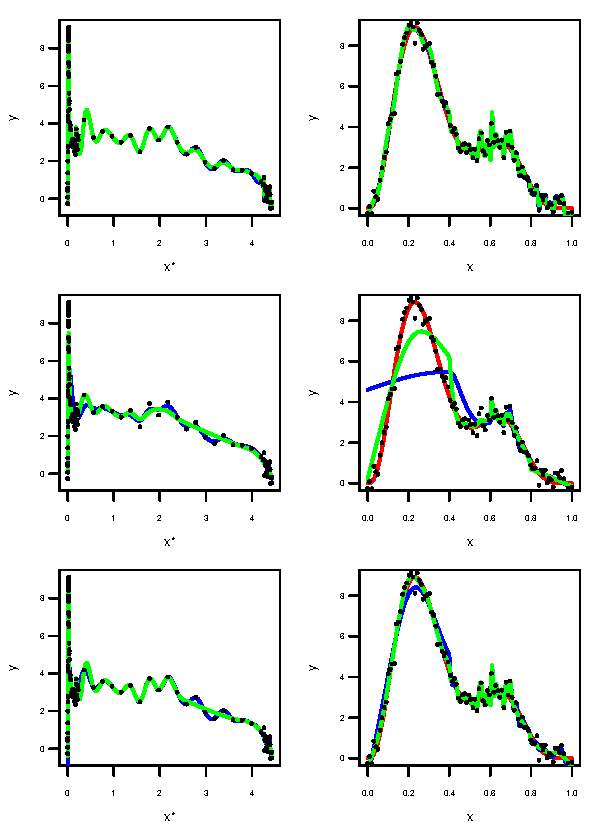
\includegraphics[width=5.5in]{mds/figs/1dedfdia.pdf} \\
\caption{Predictions in transformed and untransformed (left and right columns respectively) for \tprs\ (blue line) and penalty adjusted \tprs\ (green line) fits to the function in \eqn{hardfcn} when the smoothing parameter was pre set to give EDF of 71, 19, and 42 (top to bottom).}
\label{1dedfdia}
% generated by thesis/mds/figs/tpintexp.R
\end{figure}


\subsection{Penalty adjustments in two dimensions}

Using a similar procedures as for one dimension, the two dimensional case can be addressed. Again looking at the $ij^\text{th}$ element of $S$, for the two dimensional case we have:
\begin{equation}
S_{ij}=\int\int_\Omega \mathcal{L}^*(x,y) \Big( \frac{\partial^2 b_i(x,y)}{\partial x^2}\frac{\partial^2 b_j(x,y)}{\partial x^2}+2\frac{\partial^2 b_i(x,y)}{\partial x \partial y}\frac{\partial^2 b_j(x,y)}{\partial x \partial y}+\frac{\partial^2 b_i(x,y)}{\partial y^2}\frac{\partial^2 b_j(x,y)}{\partial y^2} \Big) \text{d}x\text{d}y.
\end{equation}
Matrices analogous to \eqn{oneDD} can be constructed using the finite differences from \eqn{bfinitediff} for differentials $x$ and $y$ individually and
\be
\frac{\partial^2 b_i(x,y)}{\partial x \partial y} = \frac{ b_i(x+\epsilon,y+\epsilon) - b_i(x+\epsilon,y) - b_i(x,y+\epsilon) + b_i(x,y)}{\epsilon^2},
\ee
for the cross term. The matrices then take the form:
\be
[D_x]_{kj}=\sqrt{\mathsf{K}(x_k,y_k)} \frac{\partial^2 b_j(x_k,y_k)}{\partial x^2},
\ee
\be
[D_y]_{kj}=\sqrt{\mathsf{K}(x_k,y_k)} \frac{\partial^2 b_j(x_k,y_k)}{\partial y^2},
\ee
\be
[D_{xy}]_{kj}=\sqrt{\mathsf{K}(x_k,y_k)} \frac{\partial^2 b_j(x_k,y_k)}{\partial x \partial y}.
\ee
So we may then express $S$ as:
\be
S=\tr{D_x}D_x + \tr{D_{xy}}D_{xy} + \tr{D_y}D_y.
\ee
Where the partial derivative evaluation points ($x_k$ and $y_k$) now form a grid for the integration to be calculated. First defining $x^\dagger_k$ and $y^\dagger_k$ analogously to \ref{midpointS}, we have:
\be
x^\dagger_k=a_x+\frac{(k-0.5)(b_x-a_x)}{K},\\
y^\dagger_k=a_y+\frac{(k-0.5)(b_y-a_y)}{K},
\ee
for $k=1,\dots,K$. The integration grid may then be constructed as:
\be
\{x_k : k=1,\dots,K\} = \{x^\dagger_1,x^\dagger_1,x^\dagger_1,\dots, x^\dagger_2, x^\dagger_2, x^\dagger_2,\dots, x^\dagger_K, x^\dagger_K, x^\dagger_K\},
\ee
\be
\{y_k : k=1,\dots,K\} = \{y^\dagger_1,y^\dagger_2, y^\dagger_3,\dots, y^\dagger_K,y^\dagger_1,y^\dagger_2, y^\dagger_3,\dots, y^\dagger_K,\dots\}.
\ee
Finally, those $(x_k,y_k)$ that do not lie inside the boundary in MDS space are removed leaving only those points that lie inside.

\subsubsection{Finding $\mathcal{L}^*$}

Calculating $\mathcal{L}^*(x,y)$ in two dimensions is more tricky than in the one dimensional case. Since the two-dimensional case is to be used in practise, the method for finding $\mathcal{L}^*(x,y)$ must depend on the MDS configuration, as the stretch factors will not be known \emph{a priori} (as was the case in the previous example).

The general idea is to make $\mathcal{L}^*(x,y)$ a function of the change in density of points caused by projecting the original space into MDS space. However, if we assume that the density in the untransformed space is $1$ everywhere, we merely need to calculate the density in MDS space. Having calculated the point density in MDS space, $\mathcal{L}^*(x,y)$ is just some function of this density.

In order to find calculate the point density in MDS space, the following steps are performed:

\begin{enumerate}
\item A grid in the original space is mapped into the MDS space. Ideally, this grid would be dense enough for it to be possible to just count the number transformed points in each square of a regular mesh. However, it would be computationally demanding to project a dense grid into MDS space, so instead a sparse grid is used and then interpolated. This consisted of taking 10 equally spaced points on each side of the square and drawing lines between points on opposing sides. Where the lines crossed were the extra points (along with those points lying on the boundary of the square itself).
\item The interpolated points are then used to estimate the overall point density in MDS space by simply counting the number of points there were in each of a set of squares made from the integration grid, call is $\mathcal{L}(x,y)$. This is shown in \fig{densgrid} for the double peninsulae domain. 
\item Then define $\mathcal{L}^*(x,y)$ as the function
\be
\mathcal{L}^*(x,y)=\frac{1}{(1+\mathcal{L}(x,y))^{3/2}}.
\ee
The $+1$ in the denominator ensures that we do not divide by zero when evaluating $\mathcal{L}^*(x,y)$. The fact that $\mathcal{L}^*(x,y)$ is then a piecewise function should not be too worrying since the aim here is to address the broader problems with the change in spatial density, not the fine-gained details.
\end{enumerate}

Note that the power is now $\frac{3}{2}$. This is since we do not know the contraction/expansion in each direction individually, but rather the overall change in area. As such we use $\frac{3}{2}$ rather than the cubic on $x$ and $y$ and unitary on the cross term.

\begin{figure}
\centering
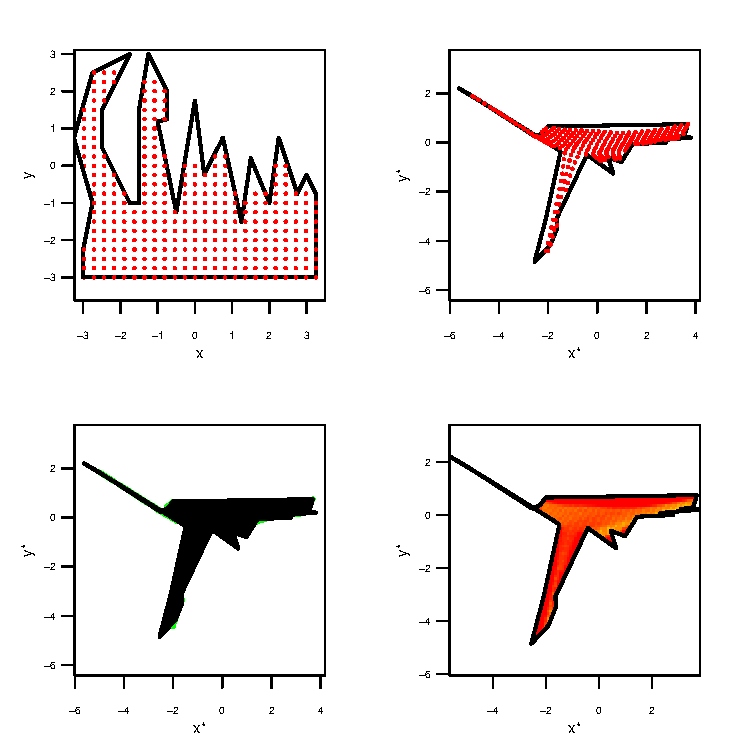
\includegraphics{mds/figs/densgrid.pdf} \\
\caption{The grids used to calculate $\mathcal{L}^*(x,y)$ for the double peninsulae domain. The red grid in the top left figure is mapped to the red grid in the top right panel. The red points in the top right are then used as the basis for the interpolation in the bottom left. The number of green points in each of the squares made from the black points in the bottom left plot are used to calculate the spatial density in that square. The heat map in the bottom right shows the values of $\mathcal{L}(x,y)$ (ie. the density of the green points), here red is low density, yellow is high. Note that some of the points lie outside of the boundary in the MDS projections. This is due to the boundary in MDS space being the straight line interpolant of the vertices of the boundary in the original space.}
\label{densgrid}
% generated by phd-smoothing/mds/wt2-intexp.R and intexp/smooth2.c.R with comments removed
\end{figure}

\subsubsection{Checking that the adjustment works}

In order to make sure that the adjustment works in both the known and unknown contraction/expansion case, a small simulation was run. In this case a surface consisting of two bivariate Normal distributions (mean vectors $(0,-0.5)$ and $(0,0.5)$, covariance matrix diagonal entries $(0.2,0.1)$) were sampled from (sample size 300) and then noise added from a $\text{Normal}(0,0.05)$ distribution. The surface was then divided into its four constituent quadrants about the origin and squashed according to the following factors (in $(x,y)$ pairs, in order top left, top right, bottom left, bottom right): ((0.3,5),(1,5),(0.3,1),(1,1)).

The samples were then used to fit a standard \tprs\ model, \tprs\ with adjusted penalty with known stretch factors and a \tprs\ with $\mathcal{L}^*(x,y)$ estimated from the data. The mean squared error between the truth and prediction over a dense (50 by 50) grid was then calculated.

The simulation results show that there is a decrease in MSE when the expansion/contraction of the space is taken into account (MSEs were: $2.355, 2.300 \text{and} 2.305$ for \tprs, known stretch and estimated stretch, respectively). Unfortunately this didn't offer the same visual improvement as the 1-dimensional case, so heat maps are not shown here.

The next section puts the adjusted penalty approach to the test on a number of domains and compares it to other possible models.

\section{Wider simulations and real data}

\subsection{Peninsulae domain}
\label{wt2bigsim}

Using the same setup as in \secref{mds-wt2-sim}, for each error level (0.35, 0.9 and 1.55), 200 realisations were generated. From these 250 samples were drawn to fit the model, predictions were over a grid of 1253 points with MSE and EDF recorded per model for each simulation. 

The models that were fitted were:
\begin{enumerate}
\item \emph{Thin plate spline}:  with basis size 140.
\item \emph{\mdsap}: using a \tprs\ with basis size 140.
\item \emph{\mdsap}: using a tensor product (see \secref{GAMtensor}) of cubic splines, each dimension of which had a basis size of 12.
\item \emph{\mdsap}: using a 3-dimensional \tprs\ with basis size 140. Here MDS was used to project the data into three dimensions rather than two.
\item \emph{\mdsap}: using a \tprs\ with basis size 140, with penalty adjustments.
\item \emph{Soap film smoother}: using 109 internal knots evenly spaced on a grid over the domain, with boundary basis size 60.
\end{enumerate}

As can be seen in \tabref{bigwt2resultstable}, the results from \mdsap\ with the adjustments are actually worse than those from just \mdsap. In all cases the \mdsap\ with adjusted penalty has a worse MSE than any of the other models; even the \tprs\ has a lower MSE in the two higher noise cases. \Fig{big-wt2-mses} shows box plots of these results.

However, all is not lost, the models using \mdsap\ with either 3-dimensional projection or the cubic regression spline are competitive across the board. In the case of the cubic regression spline, this is probably due to the tensor setup of the spline. Having a different smoothing parameter for each direction will allow the model to take care of the anisotropic space into which the data has been projected. In the high noise case the \tprs\ basis coupled with \mdsap\ has a lower and less variable MSE than the cubic regression spline, this may well be due to the \tprs\ enforcing the isotopy in a high-noise case and this constraint has lead to a less variable model being fitted, which happens to be closer to the truth in this case. As for the 3-D projection, the plots in \fig{wt2-3d-proj} show that the additional dimension allows for further separation of both a large and small peninsulae, which should help with the spatial heterogeneity as well as leakage.

A Wilcoxon signed rank test, matching pairs between realisations showed that there was a significant difference between the MSE each model and the soap film smoother. As can be seen from \fig{big-wt2-mses}, soap outperforms all of the other methods on this domain, with \mdsap\ (with 3-D projection) coming in second. 

Finally, note that there were three realisations omitted (for all models) in \tabref{bigwt2resultstable} and \fig{big-wt2-mses}. In these realisations the soap film smoother failed to fit the model due to knot placement. These can be safely removed as, in practise, the computer would inform the user that the knot placement was not appropriate and the knot layout could be altered.

\begin{sidewaystable}[p]
\centering
\begin{tabular}{c c c c c c c}
 & &  & MSE  & & &\\ 
$\sigma$  & tprs & mds+tp & mds+cr & mds+tp 3D & mds+tp+adj & soap\\ 
\hline
0.35  & 0.0832 (1e-04) & 0.0713 (5e-05) & 0.0633 (8e-05) & 0.058 (5e-05) & 0.0759 (6e-05) & 0.0598 (0.00032)\\ 
0.9  & 0.1957 (0.00017) & 0.1788 (0.00013) & 0.1652 (0.00025) & 0.1479 (0.00014) & 0.2413 (0.00022) & 0.1616 (0.00201)\\ 
1.55  & 0.3576 (0.00035) & 0.285 (0.00027) & 0.3198 (0.00063) & 0.2765 (0.00032) & 0.4778 (0.00048) & 0.245 (0.00034)\\ 
\end{tabular}
\begin{tabular}{c c c c c c c}
 & &  & EDF  & & &\\ 
$\sigma$  & tprs & mds+tp & mds+cr & mds+tp 3D & mds+tp+adj & soap\\ 
\hline
0.35  & 77.8675 (0.03803) & 80.5571 (0.04098) & 53.9331 (0.03577) & 61.3881 (0.05365) & 84.1456 (0.04092) & 55.2464 (0.04684)\\ 
0.9  & 47.0214 (0.0378) & 34.3451 (0.05633) & 31.9288 (0.03523) & 30.5663 (0.04034) & 50.6702 (0.04171) & 29.6874 (0.04514)\\ 
1.55  & 31.8803 (0.03843) & 18.3473 (0.03846) & 20.5101 (0.04256) & 19.7879 (0.03128) & 31.1969 (0.05291) & 20.3529 (0.03171)\\ 
\end{tabular}
\caption{Mean MSE and EDF for the six models fitted to the peninsula domain with standard errors (in brackets) over 200 realisations.}
\label{bigwt2resultstable}
\end{sidewaystable}

% big wt2 sim MSEs
\begin{sidewaysfigure}
\centering
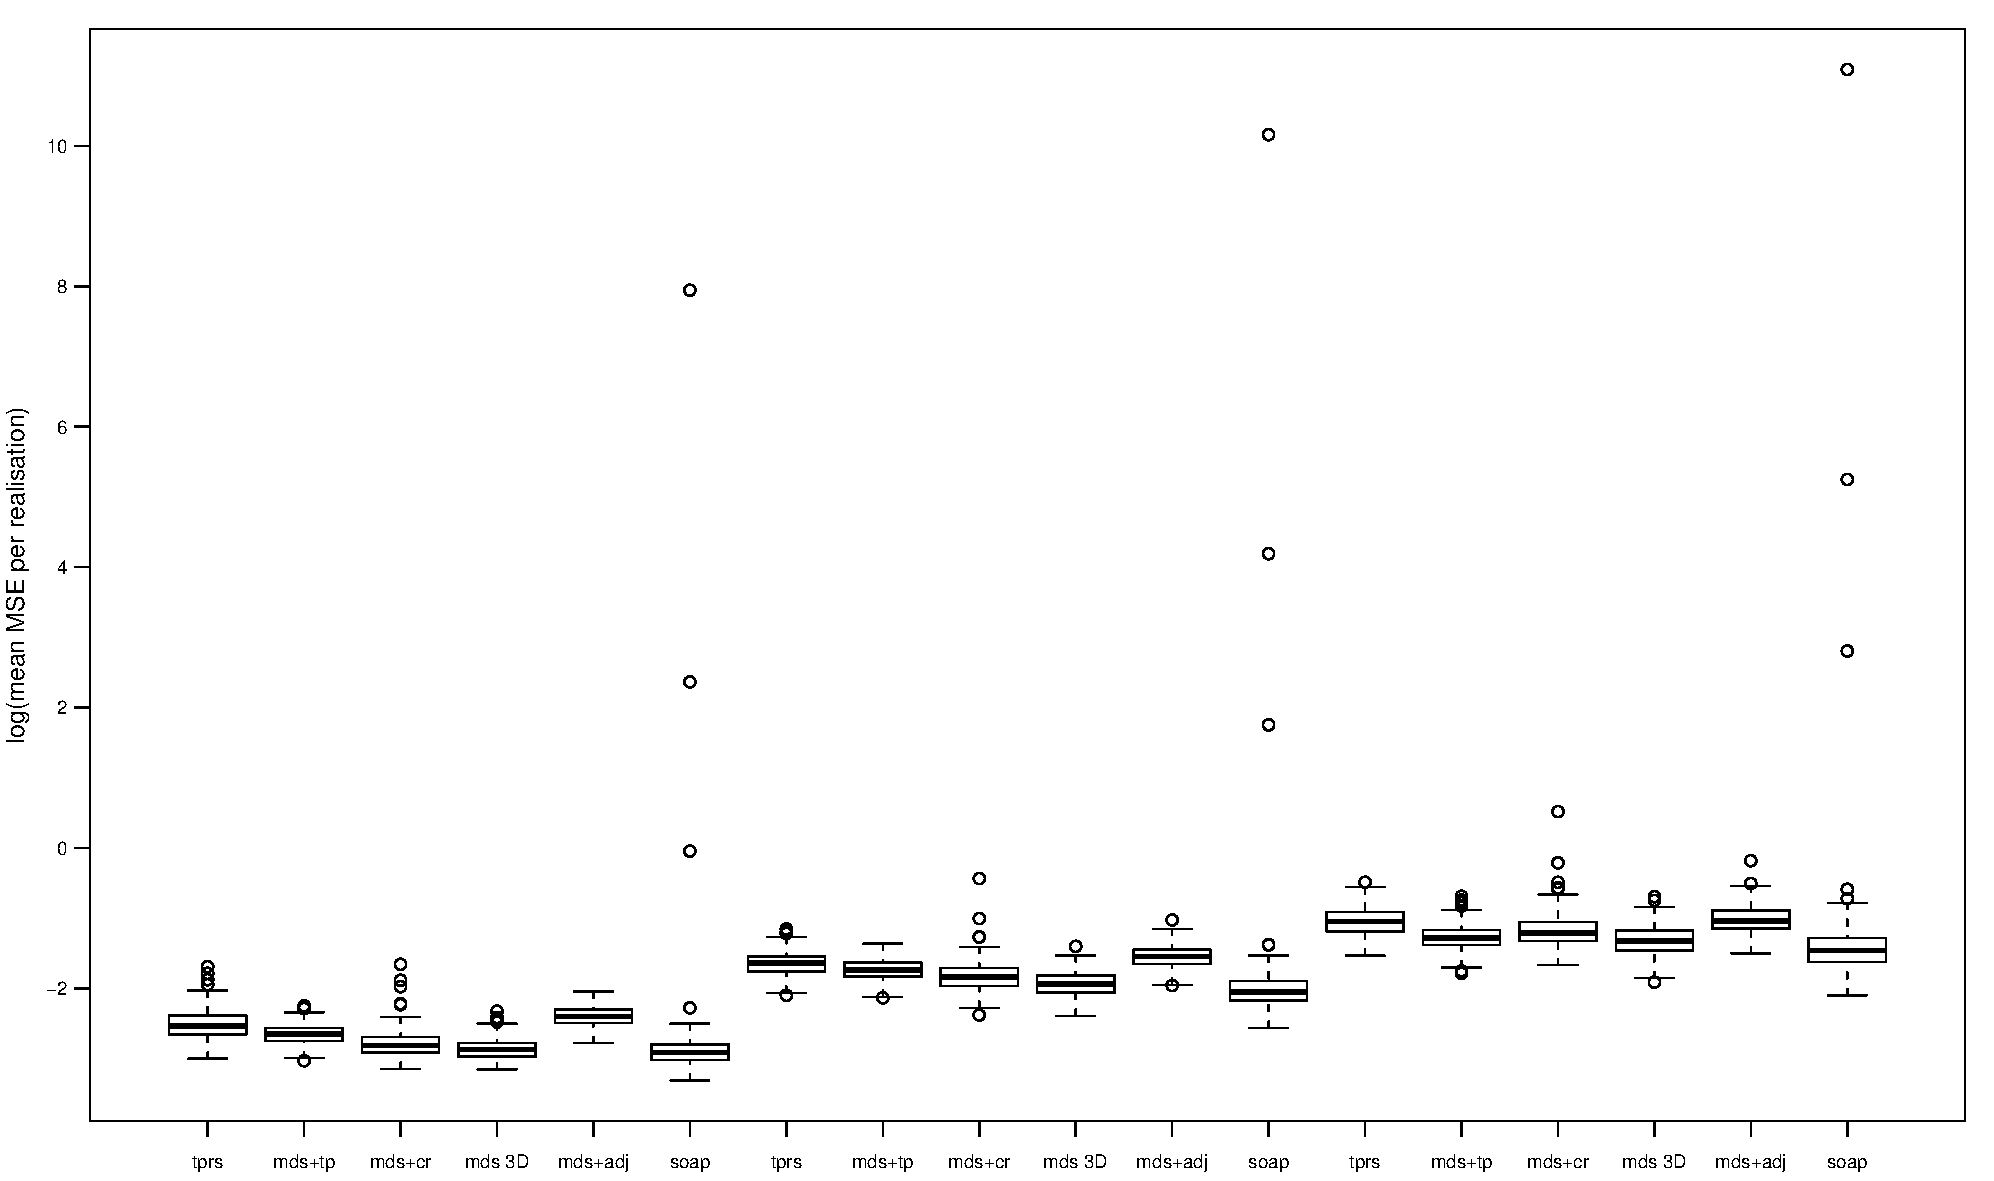
\includegraphics[width=9.5in]{mds/figs/big-mds-wt2-boxplot.pdf} \\
\caption{Logarithm of per realisation average mean squared error for the double peninsulae domain. Models are in groups of six for each error level (0.35,0.9,1.55). In all cases, a Wilcoxon signed rank test showed that MSEs for all models were significantly different from the soap film smoother ($\text{p-value} < 10^{-6}$).}
\label{big-wt2-mses}
% generate /phd-smoothing/mds/sim/boxplot-wt2.R
\end{sidewaysfigure}


\subsection{Aral sea}

The Aral sea is located between Kazakhstan and Uzbekistan. It has been steadily shrinking since the Soviet government diverted the sea's two tributaries in order to irrigate the surrounding desert in the 1960s. The NASA SeaWifs satellite collected data on chlorophyll levels in the Aral sea (\cite{soap}). The 496 data are averages of the $38^\text{th}$ 8 day observation period over the years 1998 to 2002. Smooths were fitted to the spatial coordinates with the logarithm of chlorophyll concentration (with Gamma errors) as the response.

A \tprs, \mdsap\ and soap film were all fitted to the data. In summary the setup for each model was:

\begin{enumerate}
\item \emph{Thin plate spline}:  with basis size 70.
\item \emph{Soap film smoother}: using a 12 by 12 grid of knots (74 were inside) and a boundary smooth with basis size 49.
\item \emph{\mdsap}: with basis size 70.
\end{enumerate}

\begin{figure}
\centering
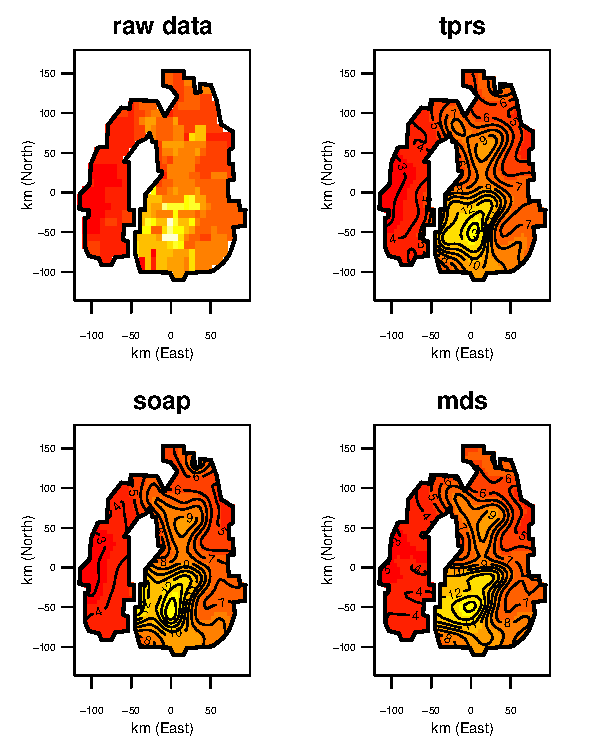
\includegraphics{mds/figs/aral-fit.pdf} \\
\caption{Raw data and predictions from the models fitted to the Aral sea chlorophyll data. Clockwise from top left: raw data, \tprs, soap film smoother, and \mdsap.}
\label{aral-fit}
% generated by phd-smoothing/mds/wt2-intexp.R and intexp/smooth2.c.R with comments removed
\end{figure}

The models were then used to predict over a grid of 496 points to create the heat maps shown in \fig{aral-fit}. The fits are broadly similar, with the \tprs\ showing some signs of leakage around (-50,-50). Both \mdsap\ and the soap film smoother combat this problem. The contour lines for all of the models look roughly the same in the main part of the sea, but in the smaller lobe, \mdsap\ is rather different from both the soap film and \tprs. 

Although the leakage is avoided, there appear to be some strange artefacts in the smooth. Ovals of higher chlorophyll appear in the smaller lobe when the \mdsap\ is fitted to the data, along with contours close to the far left of the smaller lobe. Looking at a point plot in MDS space (\fig{aral-pp}) reveals why this might be happening. As can be seen from the figure, the smaller lobe has been squashed to a line which clearly has an adverse effect on the smoother.

\begin{figure}
\centering
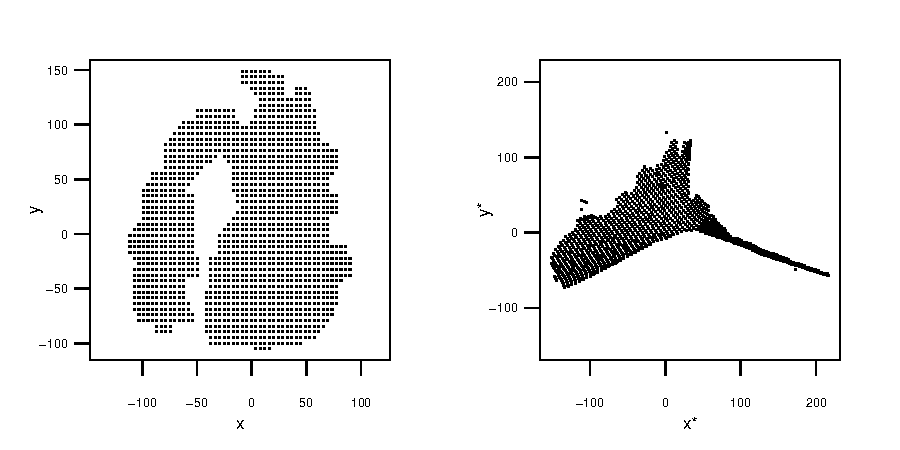
\includegraphics[width=6.25in]{mds/figs/aral-pp.pdf} \\
\caption{The prediction points for the Aral sea data set (left), with their projection into MDS space (right).}
\label{aral-pp}
% generated by phd-smoothing/mds/aral/pointplot.R
\end{figure}

The \mdsap\ with adjusted penalty was also used to fit the model, using the same settings as above. The predicted surface given by the model is shown in \fig{aral-adj-fit}. Again, the same artefacts are clearly visible in the smaller lobe of the region.

\begin{figure}[t]
\centering
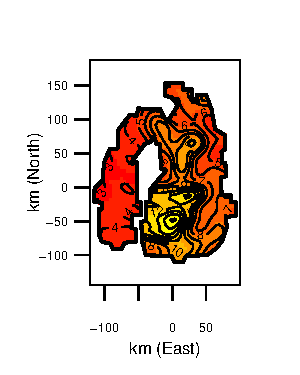
\includegraphics[width=3in]{mds/figs/aral-adjfit.pdf} \\
\caption{Predictions for the Aral sea using \mdsap\ with adjusted penalty.}
\label{aral-adj-fit}
% generated by phd-smoothing/mds/wt2-intexp.R and intexp/smooth2.c.R with comments removed
\end{figure}

Using a 3-D \tprs\ the artefacts are less prominent and the surface looks much more like the one given by the soap film smoother. Again, the three-dimensional projection shows much promise especially given the minimal extra cost to running the additional model (if the within-area distances are already calculated, only the MDS projection needs to be calculated, and the \tprs\ fitted).

\begin{figure}
\centering
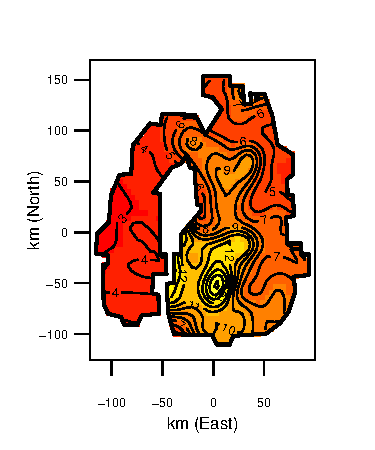
\includegraphics[width=3in]{mds/figs/aral-3d.pdf} \\
\caption{Predictions for the Aral sea using a 3 dimensional projection into MDS space for \mdsap.}
\label{aral-fit-3d}
% generated by phd-smoothing/mds/wt2-intexp.R and intexp/smooth2.c.R with comments removed
\end{figure}

\subsubsection{Aral sea simulation}

The results above show that \mdsap\ does not fit an unreasonable model, but that some artefacts do occur in the predictions. In order to further test \mdsap, a simulation was setup. Truth was set as the predictions given by fitting a kernel regression (using the \textsf{R} package \texttt{np}) to the raw data in \fig{aral-fit}. Bandwidth was selected by expected Kullback-Leibler cross-validation (\cite{hurvich}) using adaptive nearest-neighbours. A local-linear kernel regression estimator was used. 

Taking this kernel estimate as truth (see \fig{aral-np}), samples of size 100, 250 and 500 were taken and noise added from the Gamma distribution with signal-to-noise ratios 0.95, 0.75 and 0.5 (dispersion equal to 6.666,1.265 and 0.9523, and scale equal to  0.4077, 2.495 and 5.748, respectively). Predictions were then made on a grid 1498 points, from this MSEs were calculated and EDFs recorded for each model over 100 realisations.

\begin{figure}
\centering
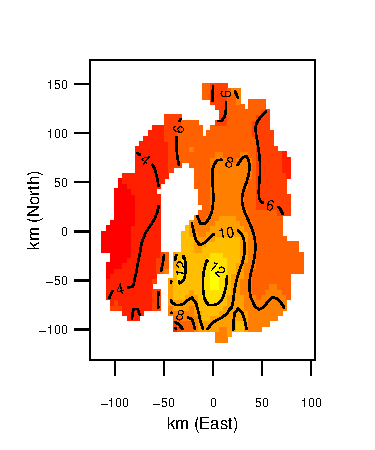
\includegraphics[width=3in]{mds/figs/aral-np.pdf} \\
\caption{The fit given by the kernel regression for the Aral sea, used as truth for simulations}
\label{aral-np}
% generated by thesis/mds/figs/aral-np.R
\end{figure}

The models fitted were as in \secref{wt2bigsim} (but with different basis sizes):

\begin{enumerate}
\item \emph{Thin plate spline}:  with basis size 70.
\item \emph{\mdsap}: using a \tprs\ with basis size 70.
\item \emph{\mdsap}: using a tensor product (see \secref{GAMtensor}) of cubic splines, each dimension of which had a basis size of 9.
\item \emph{\mdsap}: using a 3-dimensional \tprs\ with basis size 70. Here MDS was used to project the data into three dimensions rather than two.
\item \emph{\mdsap}: using a \tprs\ with basis size 70, with penalty adjustments.
\item \emph{Soap film smoother}: using 74 internal knots evenly spaced on a grid over the domain, and a cyclic spline on the boundary of basis size 25.
\end{enumerate}

% big aral sim MSEs
\begin{figure}
\centering
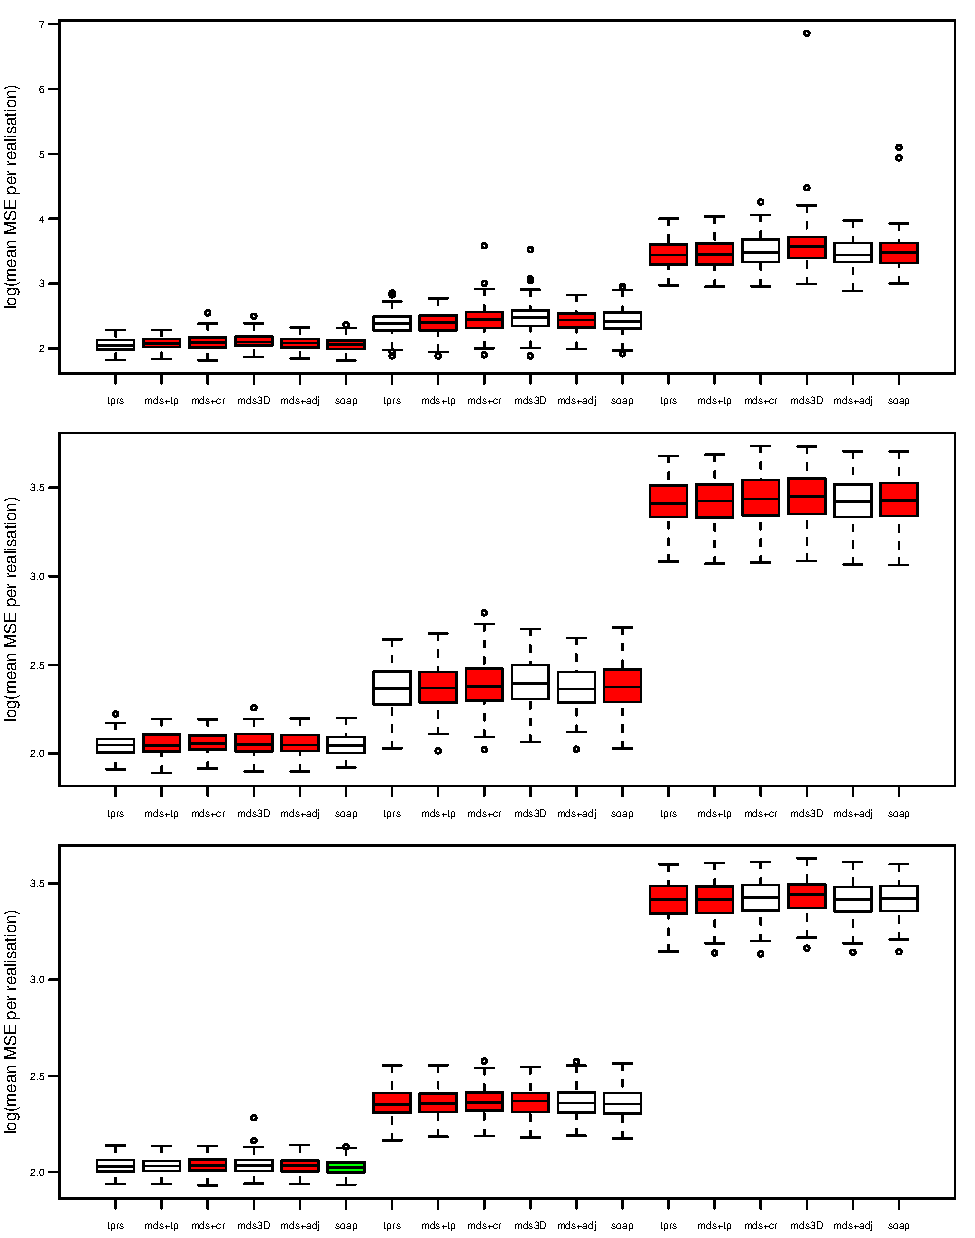
\includegraphics{mds/figs/big-aral-boxplot.pdf} \\
\caption{Box plots of the logarithm of per realisation average mean squared error for the Aral sea simulation. Top to bottom sample sizes: 100, 250, 500. Models are in groups of six for each signal-to-noise ratio (0.95,0.0.75,0.5). The shaded boxes indicate that a Wilcoxon signed rank test showed that there was a significant difference between the model and soap film smoother's MSEs ($\text{p-value} < 10^{-2}$).}
\label{big-aral-mses}
% generate /phd-smoothing/mds/aral/boxplots.R
\end{figure}

\Fig{big-aral-mses} and \tabref{bigaralresultstable} show the results of the simulations. Looking at these, there does not appear to be a clear reason to choose one of the \mdsap\ methods over the others on MSE grounds alone. Perhaps surprisingly, the \tprs\ does rather well in MSE terms, having slightly lower MSE than other models in all situations (although not significantly different from the soap film smoother ($\text{p-value} < 10^{-2}$). This is perhaps to be expected given the leakage was rather slight and localised, this combined with the \tprs\ also fitting a consistently more complex model (see EDFs, \tabref{bigaralresultstable}) may account for the superior MSE. However, we still must prefer the soap film smoother, since it does not allow any leakage. Given the evidence, above, of possible artefacts in \mdsap\ models, the soap film is looking like the best option for smoothing over regions with complex boundaries.

\begin{sidewaystable}[p]
\centering
\begin{tabular}{c c c c c c c c}
 & & &  & MSE  & & &\\ 
 $n$ & SNR & tprs & mds+tp & mds+cr & mds+tp 3D & mds+tp+adj & soap\\ 
\hline
100  &  0.95  & 7.9015 (0.08013) & 7.959 (0.07539) & 8.142 (0.09235) & 8.3365 (0.09319) & 7.9099 (0.07207) & 7.9862 (0.08923) \\ 
100  &  0.75  & 11.1357 (0.20472) & 11.2689 (0.20631) & 11.9138 (0.25673) & 12.2517 (0.24506) & 11.1778 (0.20201) & 11.5665 (0.21725) \\ 
100  &  0.5  & 32.3312 (0.71517) & 32.8335 (0.74064) & 36.3542 (1.82936) & 44.9118 (3.94612) & 32.5586 (0.67499) & 34.7731 (1.59728) \\ 
250  &  0.95  & 7.5986 (0.04417) & 7.698 (0.04591) & 7.7376 (0.04951) & 7.8235 (0.09169) & 7.8895 (0.05065) & 7.6292 (0.04719) \\ 
250  &  0.75  & 10.3526 (0.11208) & 10.5199 (0.11666) & 10.7282 (0.12681) & 10.7975 (0.13027) & 10.9595 (0.12346) & 10.5495 (0.11691) \\ 
250  &  0.5  & 31.1509 (0.4722) & 31.3645 (0.48343) & 32.2298 (0.60102) & 32.6544 (0.54744) & 30.966 (0.40946) & 31.6147 (0.50458) \\ 
500  &  0.95  & 7.6029 (0.03234) & 7.6871 (0.03205) & 7.7303 (0.03395) & 7.6631 (0.03548) & 7.6909 (0.03071) & 7.6072 (0.03209) \\ 
500  &  0.75  & 10.2918 (0.08406) & 10.4119 (0.08297) & 10.5134 (0.08788) & 10.6015 (0.11156) & 10.6991 (0.08454) & 10.373 (0.08497) \\ 
500  &  0.5  & 30.4475 (0.26024) & 30.6894 (0.26375) & 31.0089 (0.26704) & 31.3011 (0.2788) & 30.6516 (0.27123) & 30.8032 (0.26491) \\ 
\end{tabular}
\begin{tabular}{c c c c c c c c}
 & &  & EDF  & & &\\ 
$n$ & SNR & tprs & mds+tp & mds+cr & mds+tp 3D & mds+tp+adj & soap\\ 
\hline
100  &  0.95  & 29.552 (0.87023) & 21.9038 (0.67106) & 18.7032 (0.53711) & 23.254 (0.72225) & 17.3514 (0.45505) & 24.6145 (0.7117) \\ 
100  &  0.75  & 19.491 (0.98279) & 12.8962 (0.56278) & 12.0983 (0.52548) & 13.7002 (0.43143) & 10.6921 (0.34023) & 14.9221 (0.68537) \\ 
100  &  0.5  & 16.5053 (0.91097) & 11.9996 (0.94359) & 11.4546 (0.70547) & 13.7607 (0.51774) & 8.4233 (0.57631) & 12.9575 (0.69218) \\ 
250  &  0.95  & 40.9612 (0.51131) & 33.658 (0.51015) & 28.0043 (0.5445) & 37.5377 (0.63347) & 31.8296 (0.62748) & 38.2715 (0.67473) \\ 
250  &  0.75  & 24.6507 (0.68571) & 19.0361 (0.58564) & 17.6928 (0.64489) & 20.3174 (0.72174) & 17.2911 (0.74521) & 23.2137 (0.76245) \\ 
250  &  0.5  & 19.296 (0.89548) & 14.987 (0.67186) & 12.9415 (0.46289) & 15.3412 (0.6208) & 11.6872 (0.61843) & 18.3504 (1.03563) \\ 
500  &  0.95  & 50.1375 (0.39114) & 43.9809 (0.40286) & 36.0768 (0.57957) & 49.2601 (0.48478) & 42.8032 (0.44318) & 49.6045 (0.76866) \\ 
500  &  0.75  & 31.6271 (0.6354) & 26.8581 (0.72752) & 23.1292 (0.76395) & 29.2308 (0.69282) & 24.762 (0.92098) & 30.0555 (0.7023) \\ 
500  &  0.5  & 25.1535 (0.81385) & 20.7569 (0.89395) & 16.7635 (0.71303) & 20.9786 (0.91157) & 15.8003 (0.79458) & 23.2793 (1.01832) \\ 
\end{tabular}
\caption{Mean MSE and EDF for the six models fitted for the Aral sea simulation with standard errors (in brackets) over 100 realisations.}
\label{bigaralresultstable}
\end{sidewaystable}

\section{Problems with \mdsap}
\label{mds-problems}

\subsection{Why the penalty adjustment sucks}
\label{pensuck}

The simulations show that there is no big advantage of using the adjusted penalty scheme for \mdsap\ over the non-adjusted penalty. Before running the simulations, several different functions of the MDS point density were tried out. All were worse than the function that was finally settled on.

An explanation for why the penalty adjustment doesn't offer much improvement can be found by investigating the good performance of the 3-D projection model. 

Looking at the plots of the prediction points in MDS space for the peninsulae domain (\fig{wt2-2d-proj} and \fig{wt2-3d-proj}) it is easy to see that in two dimensions, the first peninsula has been squashed to a line. This is a result of the truncation performed in the MDS procedure; when we look at the 3-D projection, the peninsula clearly has width, just not in the two dimensional projection. The adjusted penalty attempts to account for this squashing of the points by allowing a more flexible model to be fit in that area. However, what is not taken into account is that some of the points in the peninsula are projected on top of each other or on the wrong side of one another. In other words, the MDS projection makes the points lose their ordering. 

As a simple, unidimensional example, take three points, $a, b, \text{and}\ c$ in the top line of \fig{linedia}. The projection could squash them in the way shown on the second line, in this case the penalty adjustments as described in \cite{wood2000} could be used to correct the model. However, with MDS we can have a situation occurring which is similar to that shown in the bottom line of \fig{linedia}, changing the order of $a, b, \text{and}\ c$. 

In the MDS projection we can see this happening in the peninsula described above. The projection takes a side-on view of the peninsula, making the points lose their ordering. In this case, the penalty adjustment can't save the model. If even the ordering of the points is not guaranteed, then the smoother's job is potentially impossible, especially once these ideas are put into two-dimensions.

\begin{figure}
\centering
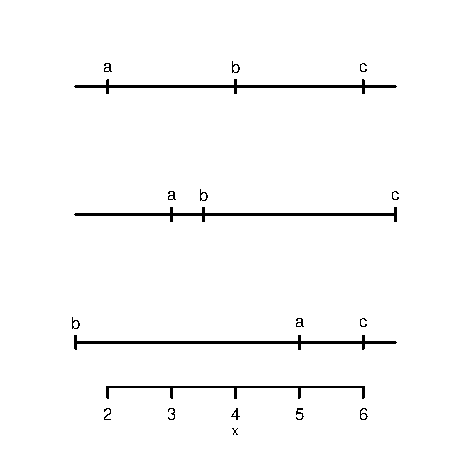
\includegraphics[width=3in]{mds/figs/linedia.pdf} \\
\caption{An illustration of how spatial mappings can squash points (middle line) and reorder them (bottom line) from their original configuration (top line).}
\label{linedia}
% generated by thesis/mds/figs/linedia.R
\end{figure}

\subsection{Why higher dimensions are not the solution}
\label{nohigherdim}

In the two cases above, moving into three dimensions allowed \mdsap\ more accurately reproduce the true function. Counteracting the phenomenon above (where the ordering of the points is lost), the extra dimension allows us to see the ``width'' of part of the domain that we take a side view of the in the 2-dimensional projection.

It seems then that there is some milage to take a 3-dimensional projection to solve this problem without the need for penalty adjustments. However, unfortunately, this is not the case. \Fig{mds-comb} shows a long domain with three peninsulae at each end. The MDS projection of the domain in two dimensions gives the points in \fig{mds-comb-2d}. There are only four peninsulae in this figure, not the six which were in the original. Using the colours in \fig{mds-comb} and \fig{mds-comb-2d}, we can see that the larger peninsulae are separated but not the smaller ones. Assuming that there is some information in the smaller peninsulae and there is reason to believe that leakage would be undesirable, this looks rather bad from a smoothing perspective.

\begin{figure}
\centering
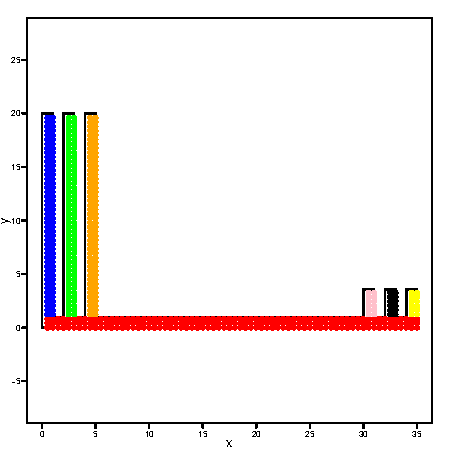
\includegraphics[width=3in]{mds/figs/comb.pdf} \\
\caption{A domain with multiple peninsulae.}
\label{mds-comb}
% generated by thesis/mds/figs/comb.R
\end{figure}

\begin{figure}
\centering
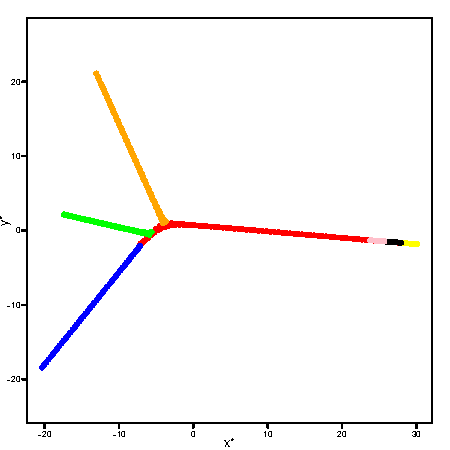
\includegraphics[width=3in]{mds/figs/comb-2d.pdf} \\
\caption{Two-dimensional MDS projection of the domain in \fig{mds-comb}, note that there are only four ``legs'' here not the six that should be there, as in \fig{mds-comb}.}
\label{mds-comb-2d}
% generated by thesis/mds/figs/comb.R
\end{figure}

So, in this case it is not unreasonable to think that an extra dimension could help. Taking a 3-dimensional projection, \fig{mds-comb-3d} is produced, however there is still no separation of the smaller peninsulae. Moving into four dimensions (\fig{mds-comb-4d}) we begin to see separation in the smaller peninsulae. However, the separation is not particularly large and leakage could still happen.

\begin{figure}
\centering
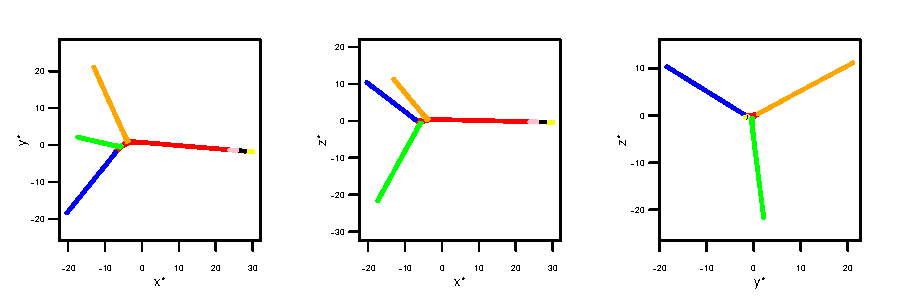
\includegraphics[width=5in]{mds/figs/comb-3d.pdf} \\
\caption{The MDS projection of the domain in \fig{mds-comb} into three dimensions. Note that there is still no separation in for the smaller peninsulae.}
\label{mds-comb-3d}
% generated by thesis/mds/figs/comb.R
\end{figure}

\begin{figure}
\centering
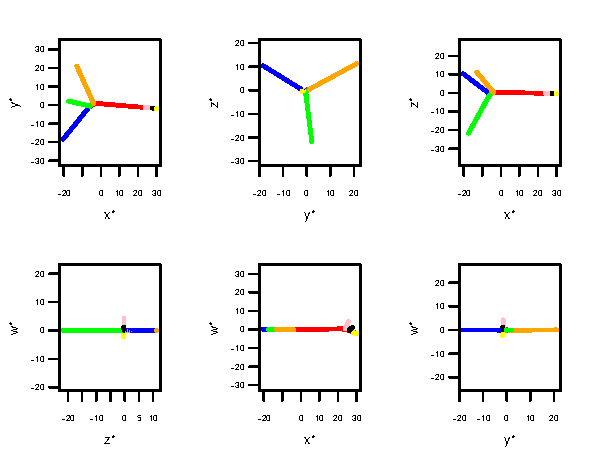
\includegraphics[width=5in]{mds/figs/comb-4d.pdf} \\
\caption{The MDS projection of the domain in \fig{mds-comb} in four dimensions.}
\label{mds-comb-4d}
% generated by thesis/mds/figs/comb.R
\end{figure}

To get a better handle on how well adding dimensions separates the peninsulae, we can use a simple quantitative measure. By comparing the mean square difference between the matrix of within-area distances and matrix of Euclidean distances in the MDS space, we can assess the amount of variation in the within-area distance being accounted for by moving into further dimensions. The criterion is calculated by taking the element-wise difference between the two matrices, squaring them and then taking the mean.

% Results here are in mds/counter/run-DRcomp.R
Looking at this measure for the domain considered in this section (the ``comb''), the Ramsay horseshoe, peninsulae domain and the Aral sea as dimension of projection is increased yields some interesting results. These are summarised in \tabref{increasek}. The table indicates that there is an optimum number of dimensions ($k$) to project into, such that adding a further dimension causes the mean squared difference between the two sets of distances to increase. However, the value of $k$ is not common to all of the domains. Indeed, the Ramsay horseshoe appears to only require two dimensions, where as the peninsulae domain appears to need five. However, we can see that this is by no means definitive, given that for the ``comb'' domain, four dimensions appears to be optimal but \fig{mds-comb-3d} shows that this doesn't offer much separation in the peninsulae.

\begin{table}[htb]
\centering
\begin{tabular}{c c c c c}
$k$ & Comb & Ramsay & Peninsulae & Aral\\ 
\hline
2 & 13.17745 & 0.04260265 & 0.3107145 &  72.4272\\ 
3 & 2.305754 & 0.09755574 & 0.06593825 & 18.87854\\
4 & 2.300667 & 0.1384483  & 0.02818498 & 14.38068\\ 
5 & 2.306849 & 0.1678546  & 0.02293624 & 14.96354\\ 
6 & 2.317045 & 0.2031276  & 0.02439487 & 15.56185 \\ 
\end{tabular}
\caption{Mean squared difference between the matrix of within-area distances and Euclidean distance in a $k$-dimensional MDS projection of the points for each of the domains detailed in \secref{nohigherdim}.}
\label{increasek}
\end{table}

Moving into continually higher dimensions seems appealing, but practically it is rather more taxing. As the dimension of the problem is increased, the order of the penalty in the GAM increases too(see \secref{GAMpenalties}). As this happens, the dimension of the nullspace of the penalty increases, meaning that more functions are unpenalised in the model. This will not lead to a simple model being fitted to the data, the real aim of \mdsap.

\section{\mdsap\ in practise}
\label{mds-prac}

Although \mdsap\ has problems, there may be some cases in which it is useful. For this reason, some practical tips on using the method are given here.

As has been seen in the previous sections, \mdsap\ does have potential pitfalls for the practitioner. Key to the whole method is that the starting grid, used to project the data into MDS space is dense enough so that the features of the domain which cause leakage are captured. In order to make sure that the initial grid is dense enough, a sparse grid over the boundary could be created and gradually made more dense grids until there are only very small changes in the plot of the grid in MDS space. Automation could be achieved by following a similar process (starting with a sparse grid and increasing the density) and at each stage checking to see if the the eigenvalues of the distance matrix have converged.

Choosing a suitable boundary is also essential to making sure that a model can be fitted in reasonable time. The more complex the boundary, the longer the shortest paths will take to calculate. Simplifying the boundary to only include those boundary vertices that are essential to combatting leakage will improve the speed of the fit.

From the analyses above, it is apparent that looking at the plots of the points in MDS space is vital to understanding whether transformation is useful and, in some cases, deciding whether a higher-dimensional projection is necessary.

\section{Conclusion}
\label{mds-conc}

This chapter has investigated the utility of using a combination of multidimensional scaling and penalised regression splines to combat the phenomenon of leakage in spatial smoothing. This was with a view to \mdsap\ being a less complex, faster, alternative to soap film smoothing, with an equally interesting motivating physical model.

As we have seen over the last two chapters, although domain transformation methods are appealing from a mathematical and physical point of view, in practise they do not appear to offer a significant advantage over existing methods and tend to produce artefacts in the resulting smooths.

\mdsap\ has the disadvantage of not calculating a fixed mapping function, as the \sch\ approach did. This leads to a large computational burden when performing prediction over a dense grid. Such an encumbrance is not desirable in a model that gives perfect predictions, let-alone one which has issues with artefacts.

Drawing together what has been learnt from the previous chapters, one can at least begin to create a list of desirable properties which would be required for a domain mapping technique to be useful for finite area smoothing. If a domain morphing technique is ever to work for smoothing over complex regions, the mapping used must have the following properties:

\begin{enumerate}
\item The mapping of points must be smooth, there should be no sudden jumps or gaps. Points that are near one-another in the original space must be near one-another in the transformed space. See (\secref{mds-smoothness}).
\item The transformation must not squash space too much. Squashing points so they are numerically indistinguishable (crowding) must be absolutely avoided, but less severe compressions of space can also cause problems. See (\secref{sch-crowding}) and (\secref{mds-penadjust}).
\item Ordering of points must be maintained. If one thinks of the points in the original space as lying on a grid, the lines joining the points may change length and orientation under the mapping, but must not cross (\secref{pensuck}).
\item A function to map one space into the other must be found. To make the method competitive in terms of computational time, the method must be able to quickly map points from the data space into the smoothing space. This, realistically, can only be achieved by using some kind of functional mapping (\secref{mds-faster}).
\end{enumerate}

Overall, it seems that \mdsap\ is simply not reliable enough to be used in practise. A method that produces artefacts could cause major problems for practitioners, incorrect inference can be extremely damaging in real world situations. The landscape of finite area smoothing over complex regions remains unchanged on the whole, the soap film smoother remains the fastest, most consistent method for performing smoothing in such situations. However, hopefully the criteria above provide some insight for those thinking of using a transformation-type approach in the future.







\chapter{Mixture model distance sampling detection functions}
% "it's another laser in your intergalactic battle cruiser" - Len Thomas

\label{chap-mmds}

\section{Introduction}
\label{s:intro}

 As was shown in chapter \ref{intro-DS}, distance sampling (\cite{IDS}, \cite{ADS}) is a suite of methods for estimating the size and/or density of biological populations. The most common approach, referred to as conventional distance sampling (CDS), is based on methods developed by \citeb{buckland92}. A commonly used extension to this methodology allows for the probability of detection to vary with covariates as well as just distance from the observer (multiple covariate distance sampling, MCDS, \cite[chapter 3]{ADS}).

Estimating the detection function is key to distance sampling. Standard distance sampling methods use the ``key function plus adjustment series'' formulation for the detection function. This can lead to unrealistic functions being fitted to the data, in particular non-monotone detection functions (as seen in \secref{intro-ds-mono}), in particular in figure \ref{fig1}.

In this chapter, a new class of distance sampling detection function models based on mixtures of simple parametric key functions is introduced. In the next section the models are described and following from that \secref{s:optimization} gives details of the optimization procedure and parametrization. Sections \ref{mmds-sims} and \ref{s:data} show the results of a simulation study and then analysis of real data, respectively. The final section gives some concluding remarks.

\section{Finite mixture model detection functions}

Following on from the definitions of the detection functions given in chapter \ref{intro-DS}, this section shows how from the definition of a mixture model detection function, the likelihood can be found for covariate and non-covariate models of both line and point transect data.

\subsection{Formulation}
\label{s:detfcts}

Denoting the detection function $g$, as before, consider a sum of $J$ mixture (detection function) components $g_j$, scaled by some mixture proportions $\phi_j$:
\begin{equation}
g(x,\mathbf{Z}; \bm{\theta}, \bm{\phi}) = \sum_{j=1}^J \phi_j g_j(x,\mathbf{z}_i; \bm{\theta}_j),
\label{mix-detfct}
\end{equation}
where $\sum_{j=1}^J \phi_j = 1$, $\bm{\phi}$ is a $J$-vector of the $\phi_j$s. As in chapter \ref{intro-DS}, the distance is denoted $x$, the $\bm{\theta}_j$s are vectors of parameters for function $g_j$, $\bm{\theta}$ is a vector of all of the $\bm{\theta}_j$s and $\mathbf{Z}$ is an $n\times K$ matrix of covariates with rows $\mathbf{z}_i$.

Here all of the $g_j$s are chosen to be half-normal functions, although other monotonic functions such as hazard-rate could be chosen (and the $g_j$s need not all have the same form). A non-covariate, $J$-point, half-normal mixture model would then be written as:
\begin{equation*}
g(x; \bm{\theta}, \bm{\phi}) = \sum_{j=1}^J \phi_j \exp \Big( - \frac{x^2}{2\sigma_j^2} \Big).
\end{equation*}
So here $\bm{\theta} = (\sigma_1, \ldots, \sigma_J)$ and there are no covariates so $\mathbf{Z}$ and $\mathbf{z}_i$ are removed.

\subsubsection{Covariates}

Covariates can be included in a similar way to MCDS (\secref{intro-ds-covar}, \cite[Chapter 3]{ADS}). Here it is assumed that each mixture component has a different scale parameter, but that the covariates affect those scale parameters in the same way. This means that the ``intercept'' term in the covariate model is different for each mixture component but the other covariates are estimated jointly for all components. Other more complex models with different covariates in each mixture component may be possible, but only the simplest model is considered here.

Analogously to \secref{intro-ds-covar}, using $i$ to subscript each observation, the formulation for the scale parameter $\sigma_{ij}$, is therefore:
\begin{equation*}
\sigma_{ij} = \exp( \beta_{0j} + \sum_{k=1}^K \beta_k z_{ik}),
\end{equation*}
where $z_{ik}$ is the $k^\text{th}$ covariate for the $i^\text{th}$ observation. As an example, for a 2-point mixture with 1 covariate, the scale parameters then have the form:
\begin{equation*}
\sigma_{i1} = \exp( \beta_{01} + \beta_1 z_{i1}) \quad \text{and} \quad \sigma_{i2} = \exp( \beta_{02} + \beta_1 z_{i1}) \text{ for } i=1,\ldots,n,
\end{equation*}
and then $\bm{\theta}_j = (\beta_{0j}, \beta_1)$ and $\bm{\theta} = (\beta_{01}, \beta_{02}, \beta_1)$. Note the similarity to (\ref{intro-ds-covar-model}).

\subsection{Likelihood}

\subsubsection{Line transects}

For line transects, given an $n$-vector of perpendicular distances $\mathbf{x}=\left ( x_1,\ldots,x_n \right )$ and associated covariate vectors $\bm{z}_i$ (the rows of $\mathbf{Z}$), the likelihood is given by:
\begin{align}
\mathcal{L}(\bm{\theta},\bm{\phi}; \mathbf{x},\mathbf{Z}) &= \prod_{i=1}^n f(x_i,\bm{z}_i; \bm{\theta},\bm{\phi}) \notag \\
&= \prod_{i=1}^n \frac{g(x_i,\bm{z}_i; \bm{\theta},\bm{\phi})}{\mu_i} \notag \\
&= \prod_{i=1}^n \frac{\sum_{j=1}^J \phi_j g_j(x_i,\bm{z}_i; \bm{\theta}_j)}{\mu_i} \label{lt-lik}
\end{align}
where $\mu_i$, the effective strip width for an observation with the same covariates as observation $i$, is given by substituting (\ref{mix-detfct}) into (\ref{intro-ds-mu-covar}):
\begin{align*}
\mu_{i} &= \int_0^w  g(x,\bm{z}_i; \bm{\theta}) \text{d}x,\\
& =  \int_0^w  \sum_{j=1}^J \phi_j g_j(x,\bm{z}_i; \bm{\theta}_j) \text{d}x,\\
& = \sum_{j=1}^J \phi_j \int_0^w  g_j(x,\bm{z}_i; \bm{\theta}_j) \text{d}x.
\end{align*}

\subsubsection{Point transects}

For point transects, with radial distances $\mathbf{r}=\left (r_1,\ldots,r_n \right )$ and associated covariate vectors $\bm{z}_i$, the likelihood is:
\begin{align}
\mathcal{L}(\bm{\theta},\bm{\phi}; \mathbf{r},\mathbf{Z}) &= \prod_{i=1}^n f(r_i,\bm{z}_i; \bm{\theta},\bm{\phi}) \notag \\
&= \prod_{i=1}^n \frac{2 \pi r_i g(r_i,\bm{z}_i; \bm{\theta},\bm{\phi})}{\nu_i} \notag \\
&= \prod_{i=1}^n \frac{2 \pi r_i \sum_{j=1}^J \phi_j g_j(x_i,\bm{z}_i; \bm{\theta}_j)}{\nu_i} \label{pt-lik}
\end{align}
where the effective area of detection for an observation with covariate vector $\mathbf{z}_i$, $\nu_i$ is defined as:
\begin{align*}
\nu_i &= 2\pi \int_0^w  r g(r,\bm{z}_i; \bm{\theta}) \text{d}r,\\
& = 2\pi  \int_0^w  \sum_{j=1}^J \phi_j r g_j(r,\bm{z}_i; \bm{\theta}_j) \text{d}r,\\
& = 2\pi \sum_{j=1}^J \phi_j \int_0^w  r g_j(r,\bm{z}_i; \bm{\theta}_j) \text{d}r.
\end{align*}

Parameters are estimated using maximum likelihood. In practice maximization is performed on the $\log$-likelihood (see \secref{s:optimization}) with analytic gradients (given in appendix \ref{app-mixderivs}).



\subsection{Estimating population size}

As in \secref{intro-ds-pop-size}, estimates of population size can be found from a Horvitz-Thompson-like estimator, all that is needed is the $p_i$s, then (\ref{HT-ds-est}) can be used. For line transects the $p_i$s are given by:
\begin{equation*}
p_i = \frac{1}{w} \sum_{j=1}^J \phi_j \int_0^w  g_j(x,\mathbf{z}_i; \bm{\theta}_j) \text{d}x,
\end{equation*}
and for point transects:
\begin{equation*}
p_i = \frac{2\pi}{w^2} \sum_{j=1}^J \phi_j \int_0^w  r g_j(r,\mathbf{z}_i; \bm{\theta}_j) \text{d}r.
\end{equation*}
Again, average detection probability for an animal within the covered region, $P_a=n/N$ can be used as a summary statistic.

%[[[Variances in both $N$ and $P_a$ were found for both non-covariate models (\cite[Appendix C]{yellowbook} TKTKTK) and covariate models (\cite[pp. 38-43]{ADS}) using standard methods set out in the literature. TKTKTK DO SOMETHING ABOUT THIS!!!]]]

\section{Optimization}
\label{s:optimization}

As noted in the literature (for example, \cite[463-480]{BDA}, \cite{robert}), mixture model likelihoods are notoriously multimodal. This multimodality can cause serious problems when finding MLEs of the parameters. To combat this a mix of optimization routines was to attempt to explore the parameter space as  much as possible.

First, simulated annealing (\cite[pp. 549-554]{numrec}) was used to explore the parameter space (for 500 iterations) then after that a quasi-Newton method (BFGS, \cite{bfgs}) was used to find the maxima (the implementations in the \textsf{R} function \texttt{optim()} were used). These two steps were run 5 times and the model with the lowest AIC was selected as the final model. This two step approach appears to be satisfactory in most cases. To aid the optimization, analytic derivatives were used by BFGS; these can be found in appendix \ref{app-mixderivs}.

\subsection{Parametrization of the mixture proportions}
\label{ds-mixpar}

When using 2-point mixtures, the constraint that the mixture proportions must sum to unity is enforced by definition (since $\phi_2=1-\phi_1$). However, in $J$-point mixtures in general, it is not guaranteed that the proportions sum to 1. The obvious way to get around this would be to add a penalty to the likelihood, should the optimization procedure propose values for the $\phi_j$s that are not in accordance with this condition. This approach is not appealing since the point of using mixtures here is to avoid penalizing or constraining the likelihood if possible. Given the problems inherent in optimizing mixture likelihoods in general, adding penalization only further complicates matters. Instead, a parametrization is used for the mixture proportions which yields $\phi_j$s that comply.

Rather than estimating the $\phi_j$s, estimate $\alpha_p$s, where the relationship between the two is:
\begin{equation*}
\phi_j = F(\sum_{p=1}^j e^{\alpha_p}) - F(\sum_{p=1}^{j-1} e^{\alpha_p}) \qquad \text{for } 1\leq j \leq J-1
\end{equation*}
and
\begin{equation*}
\phi_J = 1-\sum_{j=1}^{J-1} \phi_j
\end{equation*}
where $F$ is any continuous CDF on $(0,\infty]$. Exponentiation ensures that $e^{\alpha_p}\geq0$, so $\alpha_p$ may lie anywhere on the real line, allowing unconstrained optimisation. Summing these orders the $\phi_j$s, since only offsets are estimated. Finally, using the cumulative density function ensures that the $\phi_j$s sum to $1$. In practice the $\text{Gamma}(3,2)$ CDF is (somewhat arbitrarily) used. Figure \ref{mmds-phifig} illustrates the relationship.

\begin{figure}
\centering
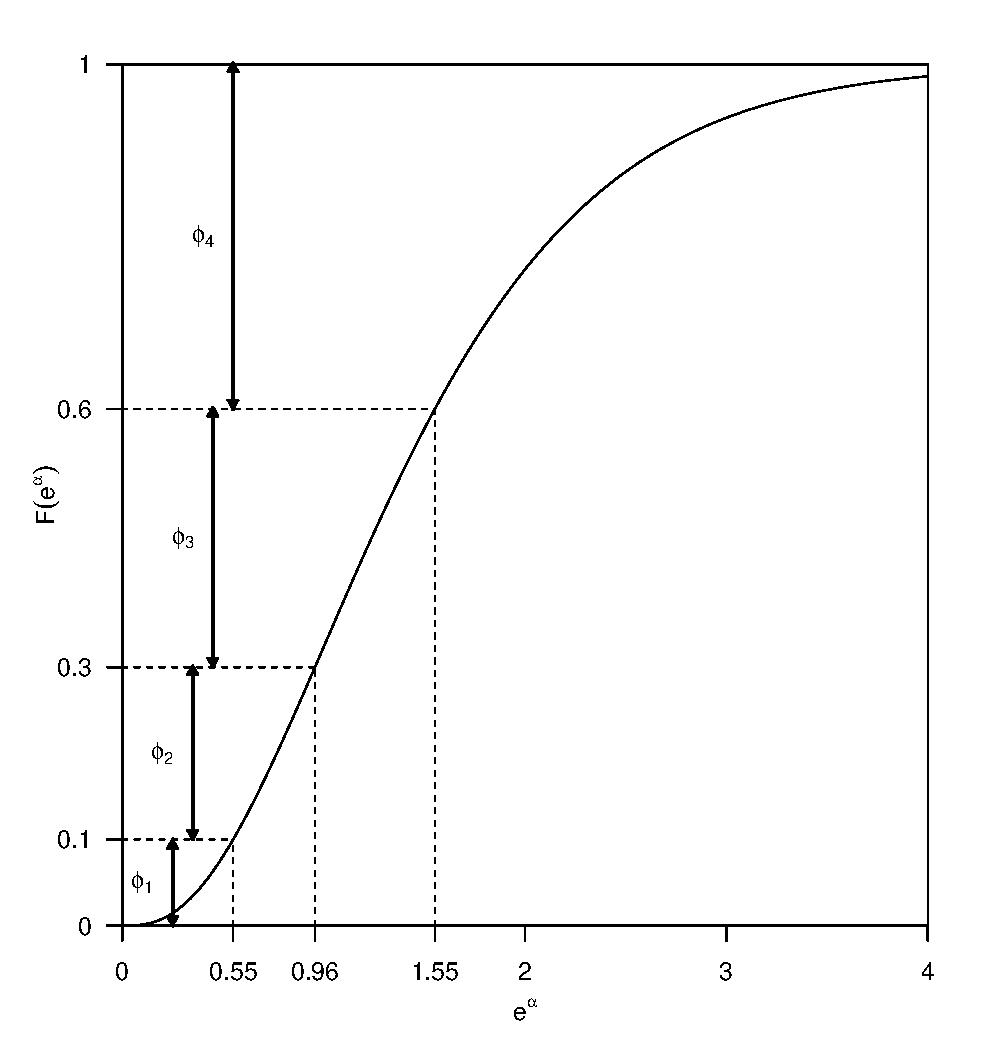
\includegraphics[width=3.5in]{mix/figs/phidia.pdf}
\caption{Illustration of the relationship between the mixture proportions, $\phi_j$ and the quantites estimated in the optimization procedure $\alpha_p$.}
\label{mmds-phifig}
\end{figure}

To transform from the $\phi_j$s back to the $\alpha_p$s by simply re-arranging the above expression.
\begin{equation*}
\phi_j = \log_e \Big(F^{-1}\Big(\phi_j + F(\sum_{p=1}^{j-1} e^{\alpha_p})\Big) - \sum_{p=1}^{j-1} e^{\alpha_p}\Big).
\end{equation*}
Note that only as many $\alpha_p$s are needed as $\phi_j$s, so no additional parameters are required.

\subsection{Starting values}

\citeb{beavers98} give a method for estimating starting values for the scale parameter of a half-normal detection function. In the non-covariate case, the estimate is given as the intercept parameter from intercept only regression on $\log(x+\frac{w}{1000})$ (where $w$ denotes the truncation distance, as above). For covariate models, the equation used for the scale parameters is used in the regression and the estimated parameters from the linear regression are used as the starting values for the $\beta$s.

A similar approach can be use in the mixture case by dividing the sorted distances into $J$ equal parts. For each of these parts a Beavers and Ramsay-type estimate is used for the $\beta_{0j}$s. The standard Beavers and Ramsay estimate using the full data was used on the other parameters. The $\phi_j$ had starting values of $1/J$ since there is no reason \textit{a priori} to believe anything else.

\section{Simulations}
\label{mmds-sims}

Extensive simulations were carried out to ensure that both parameters could be recovered and that abundance estimates were unbiased. The latter is more important than the former since our primary interest is estimating abundance. Since (as has been illustrated in \secref{intro-ds-pop-size}) the abundance depends only on the probability of detection, this was used as a target quantity to estimate and compare the results. Each simulation involved generating 200 replicate datasets from a specified mixture model using rejection sampling, fitting each dataset with 1-, 2-, and 3-point mixture models for the detection function, and in each case recording estimated (average) probability ($\hat{p}$ for non-covariate situations, $\hat{P}_a$ for covariates) of detection from the model with the lowest AIC. Rejection sampling was used to generate the observed distances (although direct simulation is also possible by rescaling the $\phi_j$s).

%\subsection{Rejection sampling scheme to simulate distances}
%
%Before going into the details of the simulation a method for generating distance data from mixture detection functions needed to be found. The cumulative distribution function of the mixture model cannot be inverted so rejection sampling (also known as the accept-reject algorithm, \cite[pp. 51-53]{montecarlostats}) was used. This is rather wasteful computationally since the proposal distribution used here is only a uniform on $(0,w)$, a proposal closer to the target could be used to increase the speed (however, this is not a major concern here). Note that direct simulation from half-normals is not possible since it is the detection functions which are mixtures rather than the PDFs. The rejection sampling scheme for $n$ samples from a mixture model detection function is as follows. 
%
%Until there are $n$ samples, perform the steps:
%\begin{enumerate}
%\item Generate $X \sim \text{Uniform}(0,w)$. 
%\item Generate $U \sim \text{Uniform}(0,1)$.
%\item Accept $X$ as coming from the PDF of distances, $f$, if 
%\begin{equation*}
%U \leq \frac{f(X,\mathbf{z}_i; \bm{\theta}, \bm{\phi})}{(1/w) M}\\
%\end{equation*}
%where $M$ is the maximum of $f$ and $1/w$ is the PDF of the proposal for $X$. Acceptance means that $X$ is within the ``envelope'' of $f$.
%\end{enumerate}
%
%In the line transect case, it is known that that the maximum value of $f$ is $1/\mu$ (since $\mu=1/f(0)$ and f(0) is the maximum of $f$), so $M=1/\mu$ (or $1/\mu_i$ in the covariate case). For point transects the maximum value of $f$ is unknown, so for each simulation the maximum was found via numerical optimization (using the \textsf{R} function \texttt{optimize()}). 

\subsection{Simulation settings}

Clearly there are many possible simulation settings that could be used. Four sets of simulations were run, which give a fairly broad range of possible scenarios.
\begin{enumerate}
	\item \textit{Non-covariate 2-point detection functions for line transect data}. Four different detection functions were tested, and are shown in the first row of figure \ref{sim-detfcts}. The first two are deliberately fairly easy to fit. The third should be harder, testing the behaviour of the model when one of the parameters is hard to estimate (the scale parameter of one of the mixture components is very large relative to the truncation distance). Finally, the fourth detection function has a large spike, which is similar to that in some of the data analysed in section \ref{s:data}.
	\item \textit{Non-covariate 2-point detection functions for point transect data}.  The detection functions were as above, with data generated as if it came from point transects. The PDFs are given in the second row of figure \ref{sim-detfcts}; the dotted lines indicate the component PDFs scaled such that the area under each curve is one.
	\item \textit{Non-covariate 3-point detection functions for line transect data}. Two different models for the detection functions were used. They are shown in the third row of figure \ref{sim-detfcts}. The first is much like the second line transect detection function, enabling us to investigate the efficacy of model selection. The second is a more complex shape that could only be created using a 3-point mixture; it has the added complication (as with the third line transect simulation) that one of the components may be non-identifiable.
	\item \textit{Covariate 2-point detection functions for line transect data}. Two different models were tested, the first of which has a binary factor covariate: half of the observations had covariate value 1 and half had covariate value 0. The second model had a continuous covariate, whose values were generated from a standard normal distribution function. Detection functions are shown in the fourth row of figure \ref{sim-detfcts}, along with the marginal detection functions for the levels/quantiles of the covariates. One goal was to test the properties of the estimator in the presence of covariates, and for these runs covariates were included in all models.  However, it is also interesting to evaluate the performance of the mixture model formulation in cases where a covariate affects detectability but the covariate is not available to the observer. Therefore the same simulated datasets were fit with mixture models that did not include covariates, and compared the resulting estimates to their with-covariate counterparts.
\end{enumerate}

\begin{figure}
\centering
\includegraphics[width=\textwidth]{mix/figs/sim-detfct.pdf}
\caption{Plots of the models used in the simulation study. Top row: detection functions for the line transect simulations with no covariates (solid lines) and their constituent mixture components (dashed lines). Second row: PDFs for the point transect simulations with no covariates (bold lines), with associated component PDFs (dashed lines) rescaled so the area under each curve is one; the detection functions are as in the top row. Third row: two 3-point mixtures for non-covariate line transect data, again with components (dashed lines). Fourth row, two covariate models, the first two panels are for a binary covariate, the second two for a continuous covariate; the first panel in each pair shows the detection function averaged over the covariates (along with the mixture components, similarly averaged; dashed lines) and the second panels show marginal detection functions with the levels (dashed) or quantiles (grey lines) of the detection function.}
\label{sim-detfcts}
\end{figure}

\subsection{Results}

Results from the simulation study are shown in figure \ref{sim-boxplots}, the boxplots therein are of the estimated detection probability ($\hat{p}$) for non-covariate models and average detection probability ($\hat{P}_a$) for covariate models. The number under each boxplot gives the proportion of AIC best models that were of the same form as the true model (i.e. same number of mixture components and the same covariates). For the first row (line transects with no covariates) we can see that in scenarios 1 and 3, both the true model and true probability of detection were recovered, even at low sample sizes. Whereas in scenarios 2 and 4 there was a positive bias in the estimates of the probability of detection as well as a lower proportion of ``correct'' models being selected by AIC. In scenario 2 and 4 most of the weight (0.7 and 0.6, respectively) is given to the larger mixture component, thus the smaller component is swamped; this would make the simulated data look as if it were generated from a 1-point mixture.

This effect can also be seen in the point transect simulations, but more severely. In this case one can see from the second row of figure \ref{sim-detfcts} that the PDFs of the distances look very much like only one of the components of the mixture. Fitting only a 1-point mixture to data from a 2-point mixture has lead to a positive bias in the detection probabilities, however this is only to expected given that data generated from such models would look like a 1-point mixture.

The 3-point mixtures show that detection function specified in scenario 1 can be easily represented using a smaller number of mixture terms. At sample sizes of 120 and lower, a 1-point mixture model dominated (around 150 of the AIC selected models were 1-point mixtures) then at the two higher sample sizes, 2-point mixtures dominated. Scenario 2 seemed more like a ``true'' 3-point data set, although only at the two larger sample sizes was a 3-point model selected more than half of the time. Interestingly at the lower sample sizes, a 2-point mixture was selected more often than 1-point (137, 173 and 182 times for the lowest three sample sizes). This effect may be due to the large, potentially non-identifiable, scale parameter being confounded with the other parameters, although this did not appear to be problematic in the scenario 2 of the line transect non-covariate models, above.

The covariate models again show an initial positive bias in $\hat{P}_a$ but do still converge to the true value at higher sample sizes. The numbers beneath the boxplots mask rather more than in the other models, since model selection was performed on not only the number of mixtures but also as to whether covariates were included in the model. Further analysis shows that at the larger two sample sizes we see that the ``true'' model is selected almost all of the time. However,  at smaller sample sizes we see more interesting behaviour. For scenario 1, at the two lowest sample sizes a 1-point non-covariate model dominates, followed by 1-point with covariates, then 2-point covariate and 2-point non-covariate. So, as one would expect, the simplest two models are selected most, but the added information from the covariates means that the 2-point covariate is selected ahead of the 2-point non-covariate. At sample size 120, the 1- and 2-point covariate models are both selected about 70 times, and the non-covariate 1- and 2-point models about 30 times. Contrary to expectations the 3-point mixtures are barely selected at all (with or without covariates) leading to the conclusion that the covariates cannot simply be substituted for further mixture terms, even in the binary covariate case. Scenario 2 shows a slightly different picture; the non-covariate models are selected less, even at lower sample sizes (the 1-point covariate model was selected 90 times a the lowest sample size) which might be expected given that scenario 2 included a continuous covariate. As was the case for scenario 1, the 3-point models were barely selected at all. In both scenarios there seems to be a bite point between a sample size of 120 and 480 where the correct model is selected almost every time.
	

\begin{figure}
\centering
\includegraphics[width=6.5in]{mix/simulations/pa-plot.pdf}
\caption{Simulation results: boxplots of the estimated detection probabilities for the best model (by AIC score). Layout is as in figure \ref{sim-detfcts}. Grey lines indicate the true value of the average detection probability. Numbers underneath each boxplot give the proportion of AIC best models that were of the same form as the model that the data was simulated from (e.g. in covariate case 1 the proportion of AIC best models that were two point mixtures that included the covariate in the model).}
\label{sim-boxplots}
\end{figure}


\section{Real data}
\label{s:data}

Given the performance of the method in simulation, four data sets were analysed using the method. They were chosen because either they exhibited non-monotonicity (\cite{williams}, \cite{pike}), were particularly spiked (\cite{ants}) or were sufficiently big that it was though they might support a mixture with many components (\cite{amakihi}). Between them they cover both covariate and non-covariate data from line and point transect surveys on boats and on foot.

\subsection{Williams and Thomas (2007) cetacean survey}

\citeb{williams} study several species of cetaceans off the coast of British Columbia. Here data for three of the species are re-analysed: harbour seal (\textit{Phoca vitulina}) in water, harbour porpoise (\textit{Phocoena phocoena}) and humpback whale (\textit{Megaptera novaeangliae}) (with truncation at 500m, 500m and 2000m respectively). Results are summarised in table \ref{williams-table} and detection functions for the models selected by AIC are shown in figure \ref{williams-detfcts}.

\begin{table}
\centering
\begin{tabular}{c c c c c c}
Species & Model & AIC & $\hat{P_a}$ & K-S $p$\\
\hline
Harbour seal & Hn+$\cos(2)$ (W\&T) & 2771.05 & 0.425 & 0.515\\
(in water) & Hn 2-pt  & 2769.86 & 0.335 & 0.945\\
Harbour porpoise & Hr (W\&T) & 690.66 & 0.212 & 0.99\\
 & Hn 2-pt & 692.09 & 0.254 & 0.99\\
Humpback & Hn+$\cos(2)$ (W\&T) & 1033.06 & 0.386 & 0.672 \\
 & Hn 2-pt & 1035.94 & 0.381 & 0.649 \\
\end{tabular}
\caption{Comparison of the results for the \citeb{williams} data. W\&T indicates the results reported in \citeb{williams}, other results are from mixture models where the number of mixture components was selected by AIC. $\cos(x)$ indicates a Cosine adjustment of order $x$.}
\label{williams-table}
\end{table}

In each case a 2-point mixture was selected by AIC to be the best model. The mixture models for the harbour porpoise and the humpback both did not perform as well as the models selected in \citeb{williams}. However, for the harbour porpoise the AIC is only different by 2, the detectability is very similar so it does not appear that much is lost by using the mixture model. In the case of the humpback, the fitted detection function is monotone, which was not the case in \citeb{williams}; this added to the fact that there is again not a huge difference in results, leads us to believe that mixture models for the detection function can be useful. Finally, for the harbour seal data, the mixture model had a better AIC than the half-normal with cosine adjustments of order 2 which was selected in the paper. 

\begin{figure}
\centering
\includegraphics[width=\textwidth]{mix/analyses/williamsplots.pdf}
\caption{Plots of the detection functions fit to the \citeb{williams} data. In each case the model selected by AIC was a 2-point mixture. Dashed lines show the mixture components.}
\label{williams-detfcts}
\end{figure}


\subsection{Wood ants in the Abernethy forest}

\citeb{ants} analyse data on two species of wood ant (\textit{Formica aquilonia} and \textit{Formica lugubris}) in the Abernethy Forest in Strathspey Scotland over the period of August--September 2003. The number of nests sighted was 150 out to a distance of 72.04m from the track line, although 45\% of the nest sightings lay within 4m of the line. As part of their analysis several different truncation distances were used and larger truncation distances led to large variance in the encounter rate estimates and hence in overall abundance estimates. This is due to the spike caused by the large number of detections close to the line.

As well as distances, three covariates were recorded: habitat type (\texttt{habitat}, a four level factor, the size (calculated as half-width of the nest multiplied by its height) of each nest (\texttt{nest.size}, continuous variable) and whether \textit{Formica aquilonia} or \textit{Formica lugubris} were observed (\texttt{species}, a two level factor). In order to avoid numerical problems due to large values of the nest size, the variable was standardised.

As can be seen from table \ref{big-results-table}, the best model by AIC was a 2-point mixture with nest size and habitat as covariates. This is not that surprising given the best CDS model (selected by AIC) in Distance was a hazard-rate with the same covariates. What is rather surprising is that the best mixture model had a better AIC than the hazard-rate, even though it has 1 more parameter (hazard-rate models have two parameters, shape and scale). This is particularly encouraging since one might expect that mixtures would give good fits but would not achieve lower AIC scores due to the number of parameters required.

\begin{figure}[t]
\centering
\includegraphics[width=\textwidth]{mix/analyses/ants-nesthab.pdf}
\caption{Plot of the detection functions for the AIC best model for the ants data set (2-point mixture with nest size and habitat as covariates). The first panel shows the average detection function (dashed lines are the two mixture components of the detection function, averaged over covariate values). The second and third panels show the quantiles (25\%, 50\% and 75\%) of nest size and the levels of habitat type respectively.}
\label{ants-nesthab}
\end{figure}

\subsection{Long-finned pilot whales}
\label{mix-pilotwhales}

\citeb{pike} analyse data on long-finned pilot whales (\textit{Globicephala melas}). There were 84 pods sighted as part of the NASS-2001 survey (of which the pilot whale was not a target). Here the data are analysed as if there were 84 individuals. The Beaufort sea state was recorded as a covariate during the survey and enter the model as either a continuous variable (\texttt{BSS}), 6 level factor (\texttt{BSS}, as a factor), a 2 level factor (\texttt{BSS3}) or a 3 level factor (\texttt{BSS2}).

A model was fit with each of these covariates, as well as a model with no covariates. A summary of the results is given in table \ref{big-results-table} and the detection function for the best model is shown in figure \ref{danpike-detfct}.

\begin{figure}[t]
\centering
\includegraphics[width=0.75\textwidth]{mix/analyses/danpike-bss2.pdf}
\caption{The (AIC) best model for the long-finned pilot whale data -- a 2-point mixture model detection function with Beaufort sea state. Left: the average detection function, right: the marginal detection function with the levels of \texttt{BSS2}.}
\label{danpike-detfct}
\end{figure}

The best model by AIC score was a 2-point mixture with \texttt{BSS2} as a covariate. Figure \ref{danpike-detfct} shows the average detection function and the marginal detection function with the levels of \texttt{BSS2}. The plot looks significantly better than the one shown in figure \ref{fig1}.

\subsection{Amakihi}
\citeb{amakihi} analyse data on the Hawaii Amakihi (\textit{Hemignathus virens}). The data consist of 1485 observations on the bird ($n=1243$ after truncation at 82.5m), collected at 41 point transects from July 1992 to April 1995. Data was also collected on three covariates: the observer (\texttt{obs}, a three level factor), minutes after sunrise (\texttt{mas}, continuous) and hours after sunrise (\texttt{has}, a six level factor).

\begin{figure}[t]
\centering
\includegraphics[width=\textwidth]{mix/analyses/amakihi-om.pdf}\\
\includegraphics[width=0.4\textwidth]{mix/analyses/amakihi-om-pdf.pdf}
\caption{Plots of the (AIC) best model for the amakihi data. Top row: detection function averaged over covariates (dashed lines are each mixture component averaged over covariates), marginal detection function showing the levels of observer (averaged over the values of minutes after sunrise) and marginal detection function for the quantiles minutes after sunrise (averaged over the levels of observer). Bottom row: PDF of distances averaged over the covariate values.}
\label{amakihi}
\end{figure}

AIC selected a two point mixture with observer and minutes after sunrise as covariates (shown in figure \ref{amakihi}), closely followed by the model with only observer as a covariate (see table \ref{big-results-table}). In this case a CDS analysis with a hazard-rate detection function using observer and minutes after sunrise as covariates beat the mixtures in AIC terms. This is not too surprising given that the mixtures use one more parameter than a hazard-rate in this situation. It is encouraging that there is such a small difference in AIC, and that covariate mixture models were selected despite the large number of parameters that such models entail.


\begin{table}
\centering
\begin{tabular}{c l c c c}
Model & Covariates & AIC & $\hat{P_a}$ & K-S $p$\\
\hline
 & ($i$) \textit{Ants} & & &  \\
Hn 2-pt & None & 754.61 & 0.183 & 0.96 \\
Hn 2-pt & \texttt{habitat} & 751.27 & 0.150 & 0.97 \\ 
Hn 2-pt & \texttt{species} & 756.59 & 0.184 & 0.94 \\  
Hn 2-pt & \texttt{nest.size} & 741.64 & 0.214 & 0.76 \\   
Hn 2-pt & \texttt{habitat} + \texttt{species} & 749.05 & 0.152 & 0.94\\ 
Hn 2-pt & \texttt{habitat} + \texttt{nest.size} & \textbf{737.27} & 0.179 & 0.72\\
Hn 2-pt & \texttt{nest.size} + \texttt{species} & 741.92 & 0.210 & 0.77\\
Hn 2-pt & \texttt{nest.size} + \texttt{species} + \texttt{habitat} & 739.77 & 0.178 & 0.68 \\
Hr & \texttt{habitat} + \texttt{nest.size} & 745.2 & 0.194 & 0.95\\
 & ($ii$) \textit{Long-finned pilot whales} & & & \\
Hn 2-pt & None & 1298.42 & 0.295 & 0.95 \\
Hn 2-pt & \texttt{BSS} & 1286.6 & 0.209 & 0.82 \\
Hn 2-pt & \texttt{BSS2} & \textbf{1284.99} & 0.211 &  0.95\\
Hn 2-pt & \texttt{BSS3} & 1296.27 & 0.27 & 0.99 \\
Hn 2-pt & \texttt{BSS} (cont.) &  1286.26 & 0.152 & 0.84\\
Hn 1-pt + $\cos(2)$& \texttt{BSS} (cont.) & 1296 & 0.37 & 0.319 \\
 & ($iii$) \textit{Amakihi} & & & \\
Hn 2-pt & None & 10805.48 & 0.283 & 0.12 \\
Hn 2-pt & \texttt{obs} & 10778.69 & 0.289 & 0.04\\
Hn 2-pt & \texttt{has} & 10807.19 &  0.282 & 0.33\\
Hn 2-pt & \texttt{mas} & 10805.11 &  0.284 & 0.31\\
Hn 2-pt & \texttt{obs} + \texttt{has} & 10782.53 & 0.283 &  0.23\\
Hn 2-pt & \texttt{obs} + \texttt{mas} & 10778.07 & 0.289 &  0.14\\
Hn 2-pt & \texttt{has} + \texttt{mas} & 10809.17 & 0.282 &  0.43 \\
Hn 2-pt & \texttt{obs} + \texttt{has} + \texttt{mas} & 10784.5 & 0.282 &  0.35\\
Hr & \texttt{obs} + \texttt{mas} & \textbf{10777.72} & 0.30 & 0.036 \\
\end{tabular}
\caption{Results for the three data sets with covariates. Bold indicates lowest AIC for each set. In each set the final model is the lowest AIC model reported in the original analysis (in Distance). Kolmogorov-Smirnov test $p$-values (KS $p$) are also given. Results are from ($i$) the wood ant data from \citeb{ants} with truncation at 25m; ($ii$) the long-finned pilot whales \citeb{pike} with truncation at 3000m, (cont.) denotes that the covariate was included in the model as continuous, otherwise covariates entered the model as factors; ($iii$) the amakihi data from \citeb{amakihi} with truncation at 82.5m. ``Hn $j$-pt'' indicated an $j$-point mixture was used. ``Hr'' indicates a hazard-rate models was used.}
\label{big-results-table}
\end{table}


\section{Software implementation - \texttt{mmds}}

All the models discussed in this article are available as an \textsf{R} package, \texttt{mmds} (Mixture Model Distance Sampling) which is available from \url{http://github.com/dill/mmds} along with documentation. Mixture model detection functions will be available in the next version of the software package Distance (\cite{distance-software}) as an additional option for modelling the detection function.

\section{Conclusion}
\label{s:discuss}

This chapter has investigated and demonstrated the utility of detection functions constructed from mixtures of half-normal functions for both line and point transect distance sampling. The method was also extended to include covariates. The formulation presented here for mixture detection functions can be simply ``dropped in'' to the existing theory and make a handy additional approach when there are issues with non-monotonicity.

It has been shown that the method performs well on both simulated and real data. In many cases the proposed model outperforms the existing CDS and MCDS models, which is surprising given that the mixture models in question often had more parameters than the CDS/MCDS models. It should be noted however, that models do not tend fit data particularly well at small sample sizes (as was found via simulation). This problem can be avoided in practice by using AIC forward selection for the number of mixtures, ensuring the simplest model is found.

In simulation 3-point mixtures did not appear to be good surrogates for missing covariate structure in the model. In general 2-point mixtures were chosen by AIC as good models. In the examples in \secref{s:data}, 2-point mixtures consistently provided the best fit, even in the case of the amakihi (which was a very large data set). Only examination of further data will show whether 3-point and higher mixtures can be supported in real data, however in CDS analyses when the key function with adjustment series formulation is used, detection functions with 5 or more parameters are rarely selected by AIC and a 3-point mixture with no covariates requires 5 parameters.

A possible extension the methodology would be to allow continuous mixtures. In that case the detection function can be modelled as:
\begin{equation*}
g(x) = \int_\mathbb{R} \varphi(\kappa) g_\kappa(x,\mathbf{Z}; \theta, \kappa) \text{d}\kappa
\end{equation*}
where $\varphi(\kappa)$ is some function which controls the mixing of $g_\kappa$. Such an approach may present significant computation issues. However, the benefits for model fitting may be considerable. Provided that an appropriate function can be chosen for $\varphi$, more flexible models could be used whilst keeping the number of parameters low. In addition, a finite mixture of both finite and continuous mixtures could be used, echoing the work of \citeb{morgan08} in capture-recapture.

Mixture model detection functions present an appealing alternative to the adjustment term approach of \citeb{buckland92} that are currently popular in the distance sampling literature. The nested nature of the models is much more elegant than adjustment terms, and using only half-normal functions as the components of the mixtures makes model choice an easier process for the investigator. As has been seen in the analysis of the long-finned pilot whales in figure \ref{fig1}, combining covariates and adjustment terms in the current MCDS formulation does not yield monotonic detection functions in the current setup. Mixture model detection functions present a way of having both flexible functional forms and including parametric effects without these problems.

In all, the methodology set out here presents a useful addition to the family of possible functions that can be used for distance sampling detection functions. The fact that the method includes the standard 1-point half-normal model as a sub-case only makes it more appealing to practitioners. Additionally, its seamless integration into the current framework (allowing goodness of fit and other statistics to be calculated relatively easily) makes it easy to include it in analyses. Hopefully, because of these factors, mixture model detection functions will be seen as one of the standard tools for those analysing distance sampling data.

\section{Acknowledgement}

This chapter of the thesis is based on the paper ``Mixture models for distance sampling detection functions'' by the author and Len Thomas of the Centre for Ecological and Environmental Modelling at the University of St Andrews and is in preparation to submit to \textit{Biometrics}. A mixture model approach to line transect detection functions without covariates was developed as part of the author's MMath thesis at the University of St Andrews under the supervision of Len Thomas. The material detailed here is a significant development from the methods developed in that thesis. 

The author would like to thank David Borchers in particular for the suggestion of the parametrization in \secref{ds-mixpar}.





\chapter{Parallel QR for additive model fitting}

Using QR update to speed up model fitting for (G)AMs. At the moment the fitting can be done in parallel but not the smoothness selection; this will be the main body of the work.

\chapter{Something else?}

If there is time.

\bibliographystyle{chicago}
\bibliography{bib-hell}

% Acknowledgements: Elle, Simon, Len, G+R, parents, all at CREEM, Jay ver Hoef? Lindesay Scott-Hayward?


\end{document}